\documentclass[a4paper, titlepage]{article}
\usepackage[a4paper,top=2.5cm,bottom=2.5cm,left=2.5cm,right=2.5cm]{geometry}
\usepackage[T1]{fontenc}
\usepackage[utf8]{inputenc}
\usepackage[italian]{babel}
\usepackage{graphicx}
\usepackage{amsmath}
\usepackage{amssymb}
\usepackage{caption}
\usepackage{circuitikz}
\usepackage{subfig}
\usepackage{adjustbox}
\usepackage{rotating}
\usepackage{booktabs, longtable,afterpage}
\usepackage{rotating}
\usepackage{makecell}
\graphicspath{ {images/} }
\begin{document}
\begin{titlepage}
	%\centering
\begin {center}

\includegraphics[width=0.40\textwidth]{Politecnico_di_Torino_-_Logo.png}\par\vspace{1cm}
	%{\scshape\LARGE Politecnico di Torino \par}
	\vspace{1 cm}
	{\scshape\Large RELAZIONE DI LABORATORIO \\DI\\SISTEMI DIGITALI INTEGRATI\par}
	\vspace{1.5 cm}
	{\huge\bfseries REALIZZAZIONE DI UNA FFT 16X16\par}
	\vspace{2.5 cm}
\end {center} 
	{\scshape\Large STUDENTI:\\AMATO GIOVANNI LUCA Matr.267511
	\\CERBAI MATILDE Matr.274908 \\CHISCIOTTI LAURA Matr.274728\\GOTI GIANLUCA Matr.269825\\\par}
	\vfill
	
	\vfill
\begin{center}
	{\large A.A. 2019-2020}
\end{center}
\end{titlepage}

\newpage
\tableofcontents
\newpage



\section{Introduzione} %REVISIONATA LAU+MATI
L'obiettivo di tale progetto è stato quello di sviluppare un'architettura $\mu$programmata capace di implementare una FFT 16x16 con blocco elementare "butterfly", che realizza le operazioni fondamentali per eseguire la Trasformata di Fourier.\\Per l'implementazione della FFT è essenziale il collegamento di molteplici butterfly, nel caso specifico 32.\\ %PROPOSTA GIANLU A In questo caso é stato necessario collegare le butterfly su 4 stadi, ognuno composto da 8 butterfly.
L'utente deve inserire i dati con un protocollo, esaustivamente definito nei paragrafi successivi, il quale deve essere ugualmente applicato sia in ingresso che in uscita.\\In tale progetto quindi, mediante la tecnica della "$\mu$programmazione", è stato possibile creare un sistema altamente dinamico e generalizzato.
\subsection{Specifiche di progetto:}

\begin{enumerate} %REVISIONATA LAU+MATI
    \item I dati in ingresso, ovvero A, B e $W^k$ (sia parte reale che immaginaria), sono definiti in forma frazionaria (-1< dato <1) ed in complemento a due su 24 bit;
    \item I dati in ingresso devono presentare almeno 2 bit di guardia;
    \item Le uscite A' e B' devono essere definite su 24 bit;
    \item Deve essere usato un sequenziatore con indirizzamento implicito;
    \item I blocchi "aritmetici" a disposizione sono: sommatore, sottrattore e moltiplicatore. Quest'ultimo può eseguire una moltiplicazione per due (x2), comportandosi come uno shifter aritmetico in modo combinatorio, oppure può eseguire una moltiplicazione classica (AxB) con due stadi interni di pipeline;
    \item Le operazioni interne devono essere effettuate con la massima precisione, quindi senza troncamento. L'arrotondamento deve essere realizzato solamente alla fine di ogni butterfly, tramite la tecnica del ROM Rounding per riportare il dato su 24 bit;
    \item I dati in ingresso devono essere presentati con un protocollo opportuno, che deve necessariamente includere un segnale di "START";
    \item In uscita i dati devono essere riportati con un protocollo opportuno, che deve necessariamente includere un segnale di "DONE";
    \item Il sistema deve presentare due modalità differenti: una modalità detta "singola" o "one shot", dove si esegue una singola FFT, ed una modalità "FULL SPEED", in cui vengono eseguite FFT consecutive alla massima velocità, senza tempi morti tra una e l'altra;
    \item Il sistema deve includere un sistema di discriminazione tra le due modalità in cui gli unici segnali di ingresso e di uscita, non considerando i campioni di ingresso X[n] e di uscita X[k], sono lo "START" e il "DONE"
    \item La Butterfly progettata deve essere utilizzata per implementare una FFT 16x16.
\end{enumerate}
\section{Cenni di teoria} %REVISIONATA LAU+MATI
\subsection{Butterfly}  
La butterfly è il blocco elementare utilizzato nell'implementazione della FFT. Tale singolo elemento esegue delle operazioni di somma e di moltiplicazione sui numeri complessi A e B, così definiti:
\begin{equation}
    A=A_{r}+jA_{i}
\end{equation}
\begin{equation}
    B=B_{r}+jB_{i}
\end{equation}
Tali termini sono moltiplicati entrambi per un fattore definito "Twiddle Factor", espresso in tal modo:
\begin{equation}
    W_N\ap{m}=\cos(\dfrac{2\pi}{N}m) -j\sin(\dfrac{2\pi}{N}m)
\end{equation}
Infatti in ingresso alla butterfly sono presenti i termini A e B, poi moltiplicati per $W^{k}$ e $W^{k+N/2}$, ritrovando così in uscita:
\begin{equation}
    A'=A+jW^{k}*B
\end{equation}
\begin{equation}
    B'=A+jW^{k+N/2}*B
\end{equation}  
Ci sono due fattori da porre in evidenza, approfonditi in Sezione 6, grazie a cui è possibile semplificare i calcoli e ridurre il numero di operazioni:
\begin{itemize}
    \item W\ap{k+N/2}=-W\ap{k};
    \item W\ap{k} è sulla circonferenza unitaria, quindi il suo valore in modulo è pari ad uno.
\end{itemize}
In conclusione, la butterfly trasforma due campioni generici tramite i Twiddle Factor in due uscite intermedie usate nei passaggi successivi della FFT.\\Di seguito è riportato lo schema di elaborazione della butterfly:
\begin{figure}[!h]
\centering
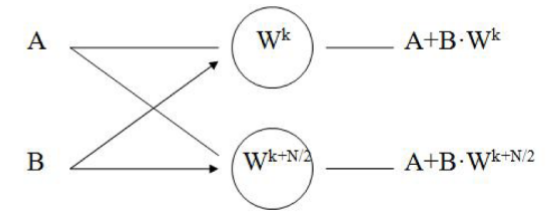
\includegraphics[scale=0.8]{butterfly.PNG}
\caption{ Struttura Butterfly}
\label{fig:Butterfly}
\end{figure}
\subsection{Trasformata di Fourier discreta} %REVISIONATA LAU+MATI  
La trasformata di Fourier discreta è definita come:
\begin{equation}
X_n= \sum_{n=1}^{N-1} x(n)e^{-j\dfrac{2\pi}{N}nk}
\end{equation}
Tale formula può essere riscritta nel seguente modo:
\begin{equation}
X_n= \sum_{n=1}^{N-1} x(n)W_N^{nk}
\end{equation}
Qui il fattore $W_N$ "Twiddle Factor", precedentemente introdotto, può essere espresso anche come:
\begin{equation}
    W_N\ap{m}=\cos(\dfrac{2\pi}{N}m) -j\sin(\dfrac{2\pi}{N}m)
\end{equation}
Data la DFT, si effettua una sua decomposizione ricorsiva in trasformate di dimensioni ridotte ogni volta della metà, dimezzando così la sua complessità ad ogni passo di ricorsione ed andando anche a ridurre la lunghezza della sequenza numerica considerata.
Tale algoritmo è estremamente lento da implementare su un sistema di elaborazione in quanto utilizza un ordine di operazioni pari a $N^2$. Però, grazie all'algoritmo Cooley Tukey, ovvero quello che implementa la Fast Fourier Transform, è possibile ridurre la complessità ad un ordine pari a $N\log_2 N$ e conseguentemente anche il carico computazionale.\\L'implementazione della FFT porta a due importanti risultati:
\begin{itemize}
    \item lo spettro immagine non è più presente tra -$\frac{f_s}{2}$ e 0, ma ora si avrà la componente a frequenza "0" in $\frac{N-1}{2}$.
    \item dato un segnale x(t) reale, la trasformata di Fourier gode della proprietà di "simmetria coniugata" ovvero risulta:
    $X(f)=X(-f)$, ovvero la parte reale della trasformata è una funzione pari e la parte immaginaria è una funzione dispari. Tale risultato sarà evidente nei risultati dei test.
    %\item lo spettro reale si ribalta, specchiandosi, mentre la parte immaginaria cambia anche di segno, come sarà presentato nella sezione "Test". 
\end{itemize}

\section{CDFD: Control Data Flow Diagram} %REVISIONATA LAU+MATI
Nell'ipotesi di avere a disposizione:
\begin{itemize}
\item un unico \textbf{moltiplicatore}  con due livelli di PIPELINE, che effettua sia la moltiplicazione di due dati (in modo pipelinato), sia la moltiplicazione di un dato per 2, agendo quindi come uno shifter aritmetico (in modo combinatorio);
\item un \textbf{sommatore} puramente combinatorio;
\item un \textbf{sottrattore} puramente combinatorio;
\end{itemize}
è stato attuato lo studio per trovare il CDFD ottimale,
%che andasse ad evitare di avere tempi morti tra una butterfly e l'altra.
in modo da ridurre al minimo il ritardo tra uno stadio e il successivo.
\\Per il completamento di un ciclo di lavoro di una singola butterfly, le operazioni necessarie sono le seguenti:  %PROPOSTA GIANLU A in modo da ridurre al minimo il ritardo tra uno stadio e il successivo, tempi morti mi suona male in una relazione. ho sostituito pure svolgimento che non mi sembrava il termine adatto
\begin{itemize}
    \item 4 moltiplicazioni classiche:\\
    $\ M\ped{1}=B\ped{R}W\ped{R}\\
       M\ped{2}=B\ped{I}W\ped{I}\\
       M\ped{3}=B\ped{R}W\ped{I}\\
       M\ped{4}=B\ped{I}W\ped{R} $
    \item 2 moltiplicazioni che compiono lo shift:\\
    $\ M\ped{5}=2A\ped{R}\\
       M\ped{6}=2A\ped{I} $ 
    \item 3 sommatorie:\\
    $\ \Sigma\ped{1}=A\ped{R}+M\ped{1}\\
       \Sigma\ped{2}=A\ped{I}+M\ped{3}\\
       \Sigma\ped{3}=\Sigma\ped{2}+M\ped{4} $
    \item 3 sottrazioni:\\
    $\ \Omega\ped{1}=\Sigma\ped{1}-M\ped{2}\\
       \Omega\ped{2}=M\ped{5}-\Omega\ped{1}\\
       \Omega\ped{3}=M\ped{6}-\Sigma\ped{3} $
\end{itemize}
Le possibili configurazioni che esistono per il CDFD sono due:
\begin{itemize}
    \item \textbf{ASAP}: As Soon As Possible, in cui ciascun operatore viene eseguito nel primo colpo di clock disponibile.\\Nel caso studiato, le somme non possono essere iniziate prima di aver terminato determinate moltiplicazioni, dato che queste fanno parte degli addendi;
    \item \textbf{ALAP}: As Late As Possible, in cui ciascuna operazione è svolta nell'ultimo colpo di clock disponibile. Ad esempio se una moltiplicazione può essere eseguita sia nel primo che nel secondo colpo si clock, nell'approccio ALAP verrà compiuta nel secondo.
\end{itemize}
Per scegliere l'approccio da impiegare si è tenuto in conto come obiettivo principale l'avere il miglior throughput possibile, cioè numero di operazioni completate al secondo, dato da $\ THROUGHPUT=\frac{1}{n T\ped{cy}} $, con n= numero di colpi di clock, anche se ciò può andare a discapito del numero di registri utilizzati.\\Sono quindi stati compiuti tre studi: ALAP con un rounder, ALAP con due rounder e ASAP con un rounder. Per ciascuno di essi è stato svolto il Variables Life Time, cioè lo studio del tempo di vita delle variabili ed è stato schematizzato il Control Data Flow Diagram.
\subsection{Caso I: ALAP con singolo rounder} %REVISIONATA LAU+MATI
Qui sono stati riportati, in Figura \ref{fig:ALAP 1}, il CDFD del caso ALAP, con l'utilizzo di un solo rounder, ed il corrispettivo studio del tempo di vita delle variabili, riportato in Figura \ref{fig:tempo di vita delle variabili ALAP 1}.\\
\newpage
\begin{figure}[!h]
\centering
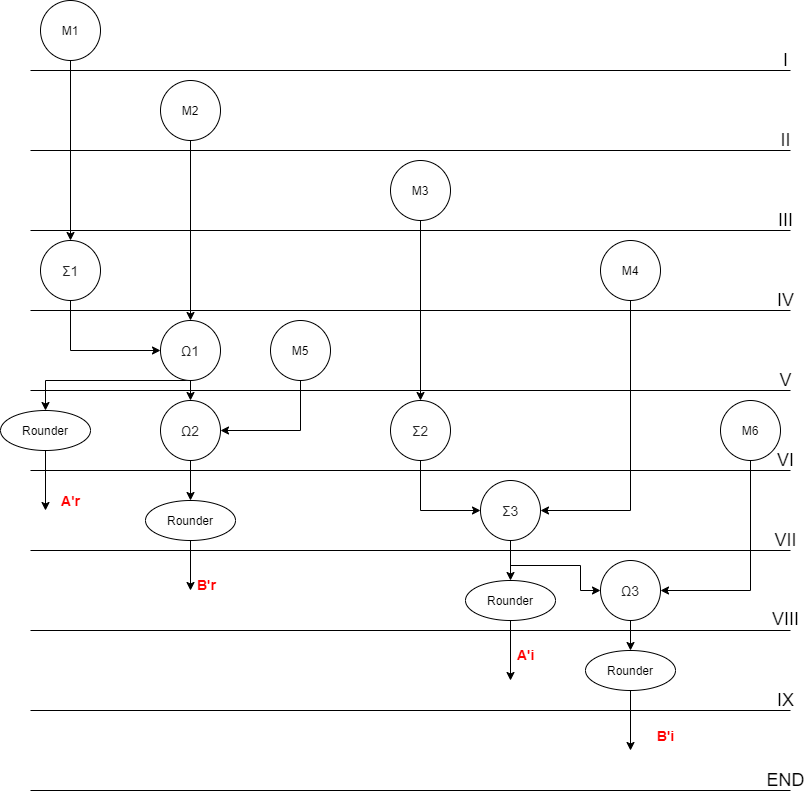
\includegraphics[scale=0.4]{DFD_ALAP 1.png}
\caption{CDFD ALAP singolo rounder}
\label{fig:ALAP 1}
\end{figure}
\begin{figure}[!h]
\centering
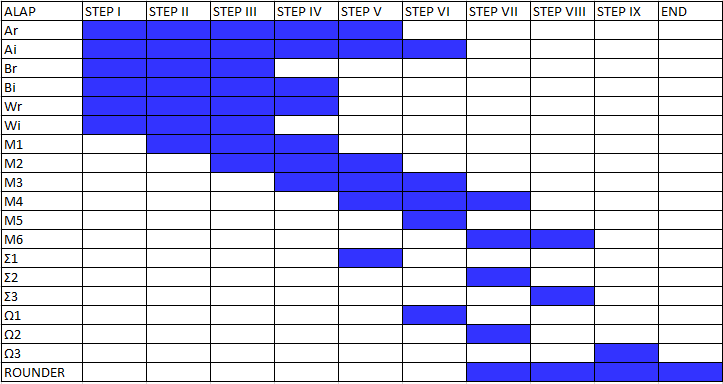
\includegraphics[scale=0.6]{Variables life time ALAP 1.PNG}
\caption{Variables life time ALAP singolo rounder}
\label{fig:tempo di vita delle variabili ALAP 1}
\end{figure}
Da tale CDFD è possibile mettere in evidenza il fatto che, avendo già dal settimo stadio il moltiplicatore nuovamente utilizzabile ed avendo l'uscita di $\Omega$\ped{2}, ovvero B'\ped{r}, disponibile all'ottavo stadio, da questo è possibile ricominciare l'esecuzione di una nuova butterfly, andando ad aumentare la velocità del sistema, senza avere tempi morti.\\Unico differimento per quanto concerne il caso ALAP, riguarda il moltiplicatore M\ped{6}, il quale non è stato posizionato all'ultimo colpo di clock disponibile, ma a quello precedente, poiché inizialmente è stato svolto lo studio non tenendo conto del Rounder e quindi B'\ped{r} risultava in uscita già dal settimo colpo di clock. Perciò, nell'ipotesi di iniziare una nuova esecuzione, spostando semplicemente tale moltiplicatore dallo step 8 allo step 7, questa sarebbe potuta incominciare già dall'ottavo stadio, evitando inutili latenze.\\Successivamente però, inserendo anche il Rounder, è stato osservato che questo causava lo slittamento di B'\ped{r} di uno step, ma è stato comunque scelto di lasciare invariata la posizione di M\ped{6}, dato che sono stati utilizzati dei registri "tampone" fissi per ogni operatore aritmetico; ciò quindi non avrebbe apportato nessun cambiamento rispetto al suo posizionamento nello step successivo.
\subsection{Caso II: ALAP con doppio rounder} %REVISIONATA LAU+MATI
Anche per questo caso lo studio è stato svolto sempre attraverso il metodo ALAP, ma, dato che le uscite B'\ped{r} e A'\ped{i} sono disponibili in contemporanea, è stato indispensabile l'utilizzo di due rounder.\\Proprio per tale necessità, questa struttura è stata ritenuta meno efficiente in termini hardware e più dispendiosa in confronto al caso precedente, il quale quindi è stato prediletto a questa.
\begin{figure}[!h]
\centering
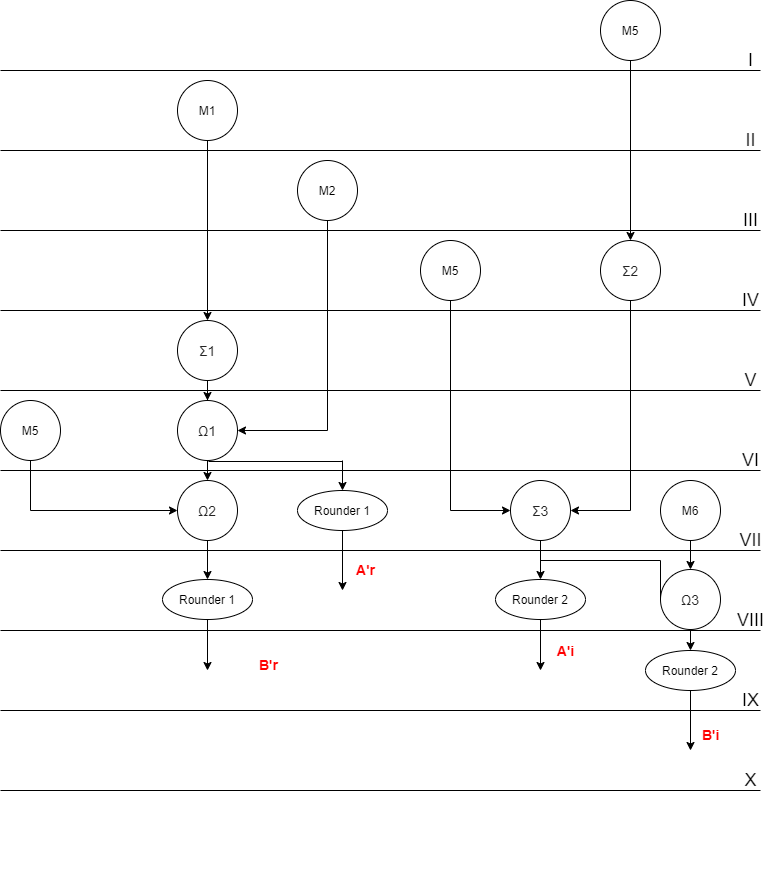
\includegraphics[scale=0.55]{DFD_ALAP 2.png}
\caption{CDFD ALAP doppio rounder}
\label{fig:ALAP 2}
\end{figure}
\begin{figure}[!h]
\centering
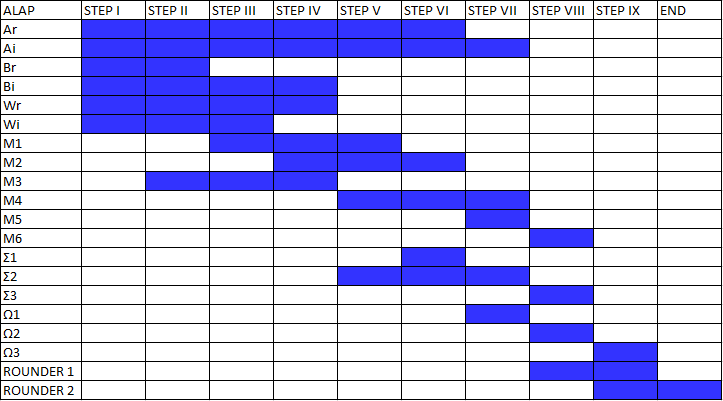
\includegraphics[scale=0.6]{Variables life time ALAP 2.PNG}
\caption{Variables life time ALAP doppio rounder}
\label{fig:tempo di vita delle variabili ALAP 2}
\end{figure}
\newpage
\subsection{Caso III: ASAP} %REVISIONATA LAU+MATI
In questo ultimo caso la struttura è stata creata utilizzando l'approccio ASAP, infatti è osservabile come gli operandi siano svolti al primo step disponibile.\\Andando ad osservare il tempo di vita delle variabili, in Figura \ref{fig:tempo di vita delle variabili ASAP}, o anche lo stesso CDFD, è possibile notare che tale metodologia necessita dell'utilizzo di uno step in più, rispetto ai due casi ALAP precedentemente riportati.
\begin{figure}[!h]
\centering
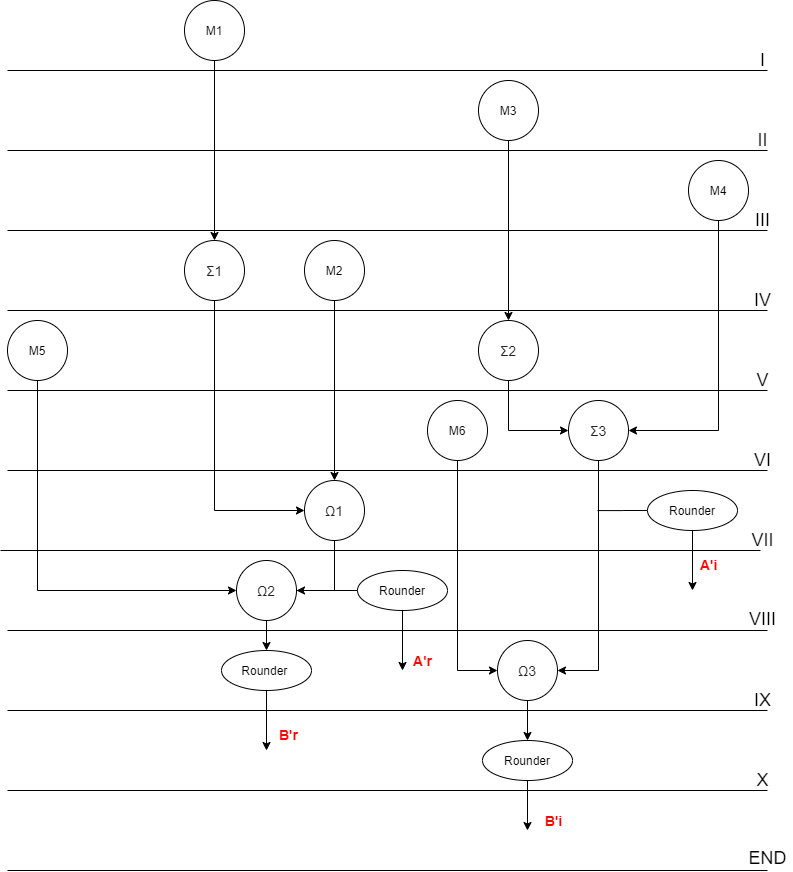
\includegraphics[scale=0.4]{DFD_ASAP.png}
\caption{CDFD ASAP}
\label{fig:ASAP}
\end{figure}
\begin{figure}[!h]
\centering
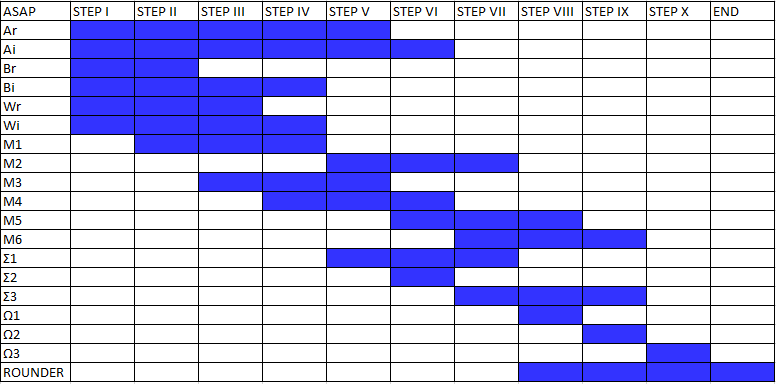
\includegraphics[scale=0.6]{Variables life time ASAP}
\caption{Variables life time ASAP}
\label{fig:tempo di vita delle variabili ASAP}
\end{figure}\\\\\\\\
Quindi, dopo aver analizzato questi 3 casi, è stato possibile concludere che l'approccio migliore da utilizzare è l'ALAP con un singolo rounder, poiché tale tecnica è quella che più ottimizza il throughput e che non necessita di un ulteriore rounder, che andrebbe solo a portare svantaggio alla struttura, sia in termini di consumi che di costi e spazio.\\Infatti mediante la configurazione scelta è possibile riutilizzare il rounder per tutte le uscite, dato che avvengono tutte in step differenti.\\
%\clearpage
\section{Analisi dei dati}
\subsection{Protocollo di arrivo dei dati}
%REVISIONATO GIANLU + LAU+MATI
Il protocollo di invio dei dati all'ingresso della Butterfly è subordinato al CDFD, per questo è stato doveroso tener conto dell'ordine di utilizzo dei vari dati esterni da parte dell'algoritmo.\\Questo utilizza nei primi due step dei valori $B'_R$ e $B'_I$, i quali dovranno quindi essere i primi dati che l'utente esterno deve inviare o che, in un'ottica più ampia, lo stato a monte deve fornire.\\Inoltre dato che il "DONE" di una Butterfly deve essere lo "START" di quella a valle è stato pensato di dare il DONE/START nel momento in cui si compie l'operazione di arrotondamento su $A'_R$.\\In team è stata presa la decisione di indirizzarsi sulla soluzione a singolo rounder, questo perchè, pur essendoci contemporaneamente due dati in uscita, ciò non ha implicato l’utilizzo di un secondo rounder, ma è stata provata la sufficienza di uno, che comporta un grosso vantaggio in termini di riduzione di spazio, comandi e ulteriori componenti.\\
Tale soluzione implica che l'arrivo dei dati sia forzato dalle data dependencies ed anche da come il Data Flow Diagram è stato costruito.\\
Una prima analisi incentrata solamente sull'osservazione delle Data dependencies e del CDFD ha inizialmente portato a sviluppare un protocollo per  i dati di arrivo, e quindi di uscita, puramente seriale con l'ordine seguente:
\begin{enumerate}
    \item $B'_r$
    \item $B'_i$
    \item $A'_r$
    \item $A'_i$
\end{enumerate}
    
 Tale soluzione però non si è rivelata corretta in quanto il sistema risultava funzionante finchè era assicurato un arrivo dei dati in modo corretto, ovvero il timing di ingresso dei dati corrispondeva al timing di uscita degli stessi, fatto garantito solo se all'ingresso A è collegato l'uscita A', stessa cosa per B e B'. Andando a collegare le Butterfly per creare l'FFT 16x16 è stato poi notato che tale condizione non risultava più garantita, infatti per alcune butterflys ad un ingresso A deve essere collegato un'uscita B' andando così a vanificare la sincronia. Questo ha portato a modificare il sistema per rendere l'uscita dei dati e il loro salvataggio completamente paralleli, con il seguente protocollo, sia per i dati in ingresso che per quelli di uscita:
\begin{enumerate}
\item $A'_R$ e $B'_R$
\item $A'_I$ e $B'_I$
\end{enumerate}
 \subsection{Scelta del numero bit di guardia} %REVISIONATA LAU
L'FFT considerata è composta da 4 stadi, quindi, se non fosse data nessun informazione riguardante questa, sarebbero necessari 2 bit di guardia per ogni stadio, quindi in tal caso 8 bit per l'intera struttura dell'FFT.\\In realtà però non sono necessari tutti questi bit, poiché è possibile dimostrare che il numero di bit di guardia sufficienti per evitare l'overflow è pari a 2 per il primo stadio ed uno per i successivi stadi, quindi generalizzando sarebbero (n+1) bit di guardia per una FFT, con n = numero di stadi.
\\Ciò avviene perchè le uscite dello step precedente rientreranno sempre nella dinamica d'ingresso dello stadio successivo e ciò è anche garantito dal fatto di avere i Twiddle Factor che si muovono sulla circonferenza unitaria, quindi il caso critico dove sia la parte reale che la parte immaginaria di W valgono 1 non si può verificare proprio per la costruzione dell'algoritmo. Questo permette quindi di diminuire il numero di bit di guardia necessari, che sono scesi da 8 a 5.
\subsection{Gestione della modalità "FULL SPEED"}
%REVISIONATO GIANLU+MATI+LAU
Nella modalità "Full Speed" il sistema deve processare nuovi campioni in modo continuo senza tempi morti, quindi è stata prevista una modalità in cui viene iniziata una nuova FFT, mentre la precedente è in fase di ultimazione. Questo equivale a implementare l'elaborazione continua sulla singola Butterfly.\\
Date le restrizioni sulle specifiche, i segnali di START e di DONE devono essere necessariamente lo stesso. Il DONE non coincide con un segnale che indica che tutte le uscite parziali sono disponibili ($A'_R,A'_I,B'_R,B'_I$), ma ha il compito di segnalare che da quel momento in avanti sono resi disponibili i dati con un certo criterio, che è pesantemente influenzato dall'algoritmo che è stato implementato.\\  
L'algoritmo realizzato fornisce in uscita:
\begin{enumerate}
\item $A'_R$ e $B'_R$
\item $A'_I$ e $B'_I$
\end{enumerate}
La Butterfly al secondo step ha bisogno di $B'_I$, ciò significa che un eventuale comando con cui si pilota l'inizio delle operazioni matematiche deve essere fornito una volta finito di campionare $B'_R$, ovvero nello step algoritmico in cui $B'_I$ è disponibile in ingresso, ma non ancora campionato, così che al prossimo colpo di clock il sistema abbia a disposizione tale dato. Quindi dal momento in cui si campiona $B'_R$, si deve aspettare un colpo di clock per campionare  $B'_I$ e questo comporta un rallentamento, in quanto sono già disponibili dei dati parziali per iniziare l'elaborazione, ma si deve ritardare il suo inizio per aspettare l'altro dato parziale del secondo step algoritmico.\\
E' stata pensata anche una soluzione alternativa, partendo dal presupposto di far lavorare le moltiplicazioni che usano lo stesso operando esterno, ovvero prima le moltiplicazioni che usano $B'_R$ e poi quelle che usano $B'_I$. Ciò permette di avere uno step algoritmico in cui non è richiesto il nuovo dato necessario ($B'_I$). In termini pratici questo comporta sicuramente un aumento dei registri temporanei da utilizzare  ed eventualmente un incremento del numero di rounder, ovvero il caso analizzato in precedenza.\\
Per iniziare una nuova operazione senza tempi morti è stato necessario analizzare il CDFD per trovare lo step algoritmico ottimale per iniziare una nuova elaborazione, che avviene sicuramente dopo l'ultima moltiplicazione, in quanto la prima operazione che viene eseguita in una nuova elaborazione è una moltiplicazione, più precisamente M1.\\ Una nuova elaborazione può iniziare solo se ha a disposizione i dati necessari che seguono lo stesso criterio esposto precedentemente, quindi, dato che M2 necessita di $B_{i}$, una nuova operazione può eventualmente iniziare nello step IX ipotizzando un tempo nullo per il salvataggio del dato in ingresso, cosa che ovviamente non è possibile. Inoltre, dato che il segnale di "START" e di "DONE" sono effettivamente lo stesso segnale, ma con l'unica differenza di appartenere a due stadi differenti, questi devono essere asseriti e "recepiti" nello stesso stato. Ciò è coerente in quanto lo "START" viene valutato dalla Status PLA per effettuare il salto, quindi in quello stato il sistema a valle deve presentare il segnale di "DONE" alto. Il timing è assicurato dalla fase negativa dell'assegnazione dei comandi, jump address e CC, questo perchè nello stato interessato la fase negativa fa alzare il "DONE", che rimane alto per tutto lo stato corrente, dove si valuta se saltare o meno nella modalità full speed, e poi viene abbassato nello stato successivo.\\ Lo "STATO 8" è lo stato adibito a generare il "DONE" e a valutare un eventuale salto. Nel caso in cui quest'ultimo non sia presente il sistema evolve nello stato in sequenza mandando in uscita i dati, se invece il sistema deva iniziare una nuova elaborazione questo andrà in uno stato dove vengono dati i comandi necessari a far uscire i dati ed in parallelo prepara il sistema a salvare i dati in arrivo. Il timing di tali operazioni è garantito in quanto oltre ai registri di interfaccia per i dati, è presente anche un flip-flop per il comando di "START". Dopo un'attenta analisi del diagramma di Stato si è calcolato che tra uno "START" e l'altro devono intercorrere 13 colpi di clock, ovvero in concomitanza dello "STATO 8" con codifica "1111".
%%%%%%%%%%%%
\subsection{Rom Rounding} %REVISIONATA LAU
Nell'analisi fatta si è cercato di capire se fosse preferibile avere un errore medio basso o un errore massimo basso (worst case). Come è noto dalla teoria, il bias error dipende da come è fatto l'algoritmo.\\Nel caso della butterfly, in ingresso sono presenti dei dati che successivamente sono oggetto di moltiplicazioni, sottrazioni, somme e dopo l'elaborazione vengono riportati in uscita, perciò l'errore considerato è quello generato internamente, e riguarda quindi la precisione.\\ L'obiettivo è stato quello di tirare fuori un errore assoluto massimo il più basso possibile per riportare il dato a 24 bit.\\Quindi, date le specifiche di progetto è stata utilizzata la tecnica del ROM ROUNDING, che definisce un arrotondamento, dati \textit{l} ingressi e \textit{l-1} uscite. Volendo  mantenere \textit{l-1} cifre, che nel caso specifico risultano essere 24, è stata creata una ROM con architettura strutturale in cui sono stati posti i dati già arrotondati.\\Perciò, seguendo il metodo utilizzato, è stata ottenuta una ROM con 2$^{l}$ righe di \textit{l-1} bit ciascuna.\\In accordo a quanto deciso, si è scelto di far entrare un numero limitato di bit.\\Il bias error potrà essere calcolato con la formula:
\begin{equation}
e_{bias}=\frac{1}{2}\left [ \frac{1}{2}^{d} -\frac{1}{2}^{l-1}\right ]
\end{equation}
Nel caso analizzato, per trovare il valore più adeguato di \textit{l}  e \textit{d}, sono state considerate varie possibilità, per poi andare a scegliere quello che risultava essere più consono per l'elaborazione realizzata. Considerando che i dati risultano essere oggetto di varie operazione aritmetiche, questi eccedono la dinamica iniziale e perciò è necessario che siano riportati su 24 bit.\\Il valore dell'errore massimo è stato quindi da subito identificato come lo stesso per qualsiasi numero di bit scelto per realizzare la ROM e pari ad un valore di $\frac{1}{2^{25}}$, infatti l'errore massimo ha dipendenza sempre dal primo bit che viene eliminato nell'operazione di arrotondamento, poiché tutti i bit successivi al primo avranno un peso minore.\\Sono state riportate in tabella i risultati ottenuti andando a variare i parametri di \textit{l} e \textit{d}, dove con \textit{X} si indica la parte che non entra nella ROM e con \textit{d} ci si riferisce al numero di bit successivi al ventiquattresimo, cioè quelli che si vuole eliminare:\\
\begin{longtable}{*3c}
\caption{Analisi bias error con l=6}
\label{tab:Analisi bias error variando i parametri l e d}\\
\toprule
Dato & d & Bias error\\
\midrule
\endfirsthead
Dato & d & Bias error\\
\midrule
\endhead
\midrule
\endfoot
\bottomrule
\endlastfoot
X0.00000 & 5 & 0 \\ 
X00.0000 & 4 & $\frac{1}{64}$ \\ 
X000.000 & 3 & $\frac{3}{64}$  \\ 
X0000.00 & 2 & $\frac{7}{64}$ \\ 
X00000.0 & 1 & $\frac{15}{64}$ \\ 
\end{longtable}
\begin{longtable}{*3c}
\caption{Analisi bias error con l=5}
\label{tab:Analisi bias error con l=5}\\
\toprule
Dato & d & Bias error\\
\midrule
\endfirsthead
Dato & d & Bias error\\
\midrule
\endhead
\midrule
\endfoot
\bottomrule
\endlastfoot
X0.0000 & 4 & 0 \\ 
X00.000 & 3 & $\frac{2}{64}$ \\ 
X000.00 & 2 & $\frac{6}{64}$ \\ 
X0000.0 & 1 & $\frac{14}{64}$ \\ 
\end{longtable}
\begin{longtable}{*3c}
\caption{Analisi bias error con l=4}
\label{tab:Analisi bias error con l=4}\\
\toprule
Dato & d & Bias error\\
\midrule
\endfirsthead
Dato & d & Bias error\\
\midrule
\endhead
\midrule
\endfoot
\bottomrule
\endlastfoot
X0.000 & 3 & 0\\ 
X00.00 & 2 & $\frac{1}{16}$ \\
X000.0 & 1 & $\frac{3}{16}$ \\
\end{longtable}
Dall'analisi delle tabelle sopra è stato evinto che l'errore medio scende al diminuire del valore di \textit{l}, ma per lo stesso valore di \textit{d}.\\
Soffermandoci però sull'azzeramento del bias error, è stato possibile giungere alla conclusione che tale valore sia pari a 0 nei casi in cui \textit{d}=\textit{l-1},%da mettere come equazione
ciò è stato ulteriormente confermato anche dalla lettura e dallo studio dell'articolo "ROM-ROUNDING: A NEW ROUNDING SCHEME" di Kuck, Parker e Sameh.
\\Quindi è stato scelto \textit{l}=6 e \textit{d}=5, realizzando così una ROM da 32 righe, ognuna composta da 5 bit, per non implementare una ROM né troppo "pesante" né che non tenesse conto di un numero sufficiente di bit per arrotondare il dato. Il metodo di arrotondamento utilizzato è il \textbf{round to nearest even}, secondo il quale se e solo se si è a metà dell'intervallo si arrotonda all'intero pari più vicino, altrimenti si effettua l'arrotondamento \textbf{half up}, che prevede una somma nel bit immediatamente dopo a quello che si intende mantenere.\\In uscita da tale memoria, dopo l'elaborazione, sarà quindi riportato solo il ventiquattresimo bit arrotondato.
%\subsection{Analisi worst case }
%%Considerando che la dinamica dei bit in ingresso deve essere compresa tra +1 e -1,\\
%Si è voluto analizzare il worse case del percorso del DFD per calcolare il numero massimo di bit che si avrà all'uscita di ogni butterfly.I dati utilizzati saranno su 24 bit:le operazioni che vengono effettuate sono moltiplicazioni, sottrazioni e somme. Nelle operazioni analizzate si è voluto ipotizzare sempre che addendi e sottraendi non raggiungeranno mai il valore massimo, cioè 47. \\
%\begin{itemize}
%\item Percorso 1: \\M1= 47 bit, registri e pipe di M1 sono da 47 bit\\$\Sigma$1 ha parallelismo con 47 bit\\M2 ha registri e pipe a  47 bit, $\Omega$1 ha sempre parallelismo a 47 bit. Si ha M5 da 47 bit e $\Omega$2 da 47 bit
%\item Percorso 2:\\M3= 47 bit, registri e pipe di M3 sono da 47 bit\\$\Sigma$2 ha parallelismo con 47 bit\\M4 ha registri e pipe a  47 bit\\ $\Sigma$3 ha sempre parallelismo a 49 bit.Si ha M6 da 47 bit e $\Omega$3 da 47 bit
%\end{itemize}
%Si è concluso che il numero massimo di bit che si andrà ad utilizzare sarà 47.
%\newpage
\subsection{Parallelismo}%REVISONATA LAU+MATI
Per il parallelismo sono state fatte valutazioni sul numero di bit per ogni operazione di ogni step.\\
Il valore del numero di bit necessario per ogni operazione è successivamente riportato:
\begin{itemize}
\item STEP I: M1=24bit*24bit=48bit;
\item STEP II:M2=24bit*24bit=48bit;
\item STEP III:M3=24bit*24bit=48bit;
\item STEP IV:M4=24bit*24bit=48bit; $\Sigma$1=24bit+48bit=48bit;
\item STEP V:M5(shift)=25bit, dato che lo shift incrementa solo di 1 il numero di bit; $\Omega$1=48bit-48bit=48bit;
\item STEP VI:M6(shift)=25bit; $\Sigma$2=24bit+48bit=48bit; $\Omega$2=25bit-48bit=48bit;
\item STEP VII:$\Sigma$3=48bit+48bit=49bit;
\item STEP VIII:$\Omega$3=25bit-49bit=49bit.
\\Dato che il massimo numero di bit necessario è 49 bit, per avere massimo parallelismo si è deciso che all'ingresso del sommatore e del sottrattore e in uscita dal moltiplicatore, sommatore e sottrattore ci siano 49 bit. Tale processo è in alcuni casi realizzato mediante l'operazione di 'resize'.
\end{itemize}
%%%%%%%%%%%%%%%%%%%%%%%%%%%%
\newpage
\section{Data Path}%REVISIONATA MATI+LAU
In questa sezione sono state analizzate le varie soluzioni progettuali adottate nel datapath.
Il datapath può essere suddiviso schematicamente come segue:
\begin{itemize}
    \item Sezione di interfacciamento e salvataggio, composto dai registri di ingresso e dal register file;
    \item Sezione aritmetica, composta da tutti i blocchi aritmetici con i relativi registri e multiplexer;
    \item Sezione di rounding;
    \item Sezione di splitting dei dati in uscita;
\end{itemize}
Nella Figura \ref{fig:datapath} è possibile osservare il datapath completo.
\begin{figure}[h]
   \centering
    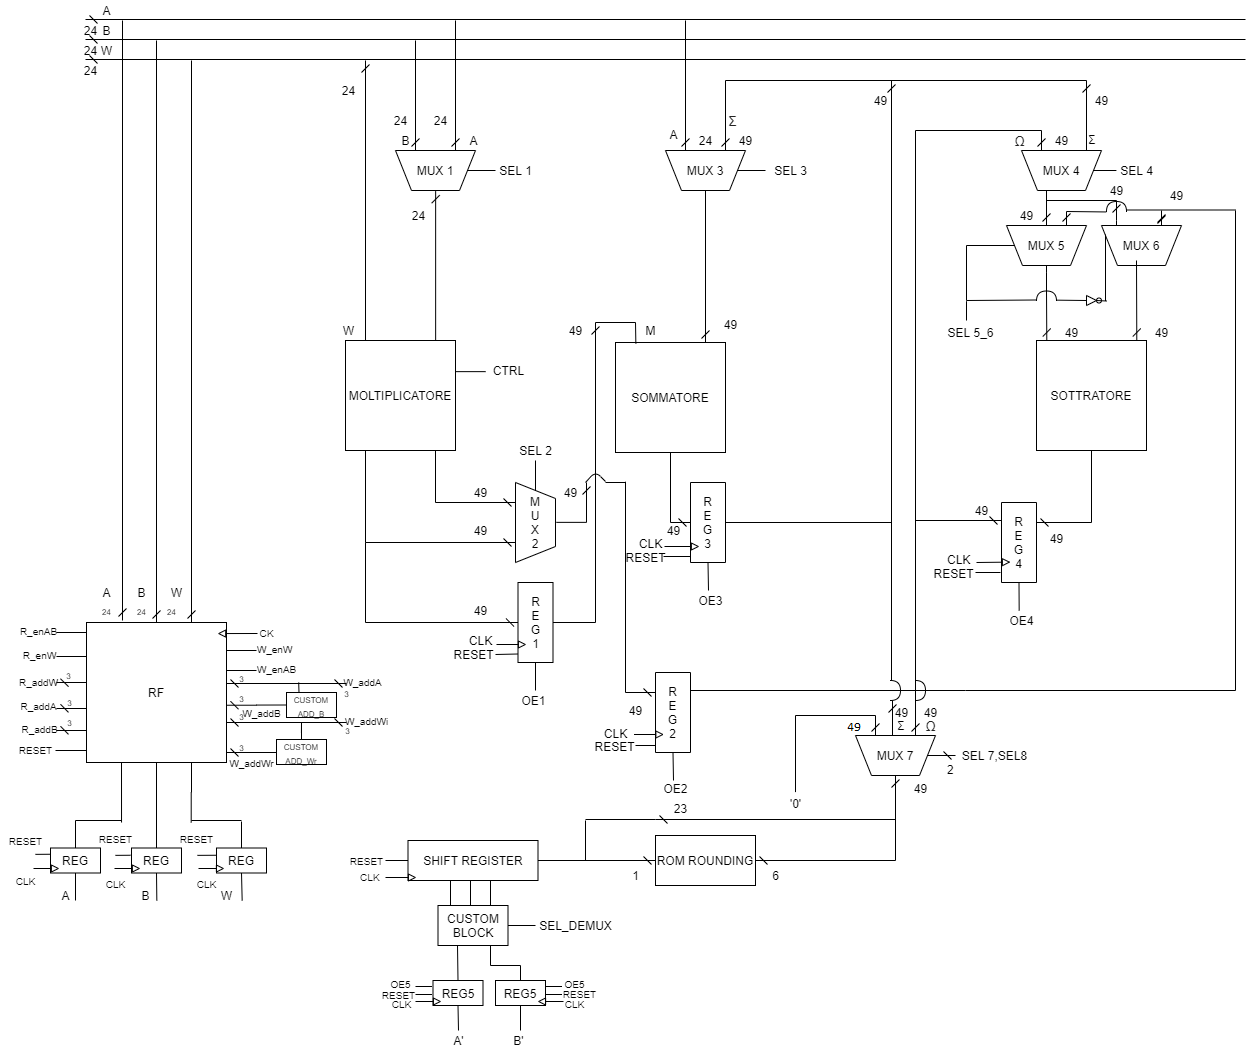
\includegraphics[scale=0.5]{DATAPATHULTIMAVERSIONE .png}
    \caption{Data Path Butterfly}
    \label{fig:datapath}
\end{figure}
\newpage
\subsection{Legenda Data path} %REVISIONATA LAU+MATI
In tale sezione si è voluto porre una breve legenda in riferimento al data path sopra riportato, in modo da rendere più facilmente accessibile all'utente l'utilizzo e la comprensione della struttura.\\I blocchi utilizzati sono i seguenti:
\begin{itemize}
    \item REG: registri non dotati di enable;
    \item REG 1, REG 2, REG 3, REG 4, REG 5: registri controllati da un enable, indicato per ognuno di essi rispettivamente con OE1, OE2, OE3, OE4 ed OE5;
    \item RF: Register File;
    \item CUSTOM ADD\_B, CUSTOM ADD\_W\ped{r}: blocchi utilizzati per ridurre il numero di bus di indirizzo;
    \item MUX 1; MUX 2, MUX 3, MUX 4, MUX 5, MUUX 6, MUX 7: multiplexer controllati rispettivamente da SEL 1, SEL 2, SEL 3, SEL 4, SEL 5\_6, SEL 7, SEL 8. A seconda del valore assunto dai SEL, i MUX selezionano un determinato ingresso;
    \item MOLTIPLICATORE: blocco in cui, mediante il controllo CTRL, viene svolta la moltiplicazione classica o x2;
    \item SOMMATORE: blocco combinatorio in cui viene svolta la somma di due addendi;
    \item SOTTRATTORE: blocco combinatorio in cui viene svolta la sottrazione di due sottraendi;
    \item ROM ROUNDING: blocco mediante il quale si attua il processo di Rom Rounding;
    \item SHIFT REGISTER: registro a scorrimento, composto internamente da 4 registri da 24 bit;
    \item CUSTOM BLOCK: blocco che, a seconda del valore assunto dal controllo SEL\_Demux, seleziona due dei tre ingressi.
\end{itemize}
\subsection{Registri di interfacciamento e Register File}%REVISIONATA MATI+LAU
Per prima cosa è stato deciso di inserire dei registri di interfacciamento sui dati di ingresso e di uscita così da essere svincolati dal mondo esterno, fare ciò è in generale una buona norma in qualsiasi progetto.\\ Oltre a questi, è stato inserito un registro sul comando di "START" in quanto, avendo ritardato i dati di ingresso, il sistema partirebbe con un colpo di clock in anticipo rispetto all'effettivo arrivo dei dati all'interno del sistema.\\
Per il salvataggio dei dati di ingresso e dei Twiddle Factor è stato adottato l'uso di un Register File composto da 6 registri, ognuno da 24 bit. La scelta del numero di porte di ingresso da utilizzare è stato particolarmente difficile da determinare. Infatti inizialmente, avendo scelto un protocollo puramente seriale, era stato deciso di avere:
\begin{itemize}
    \item una singola porta per Twiddle Factor "W", dove veniva salvata prima la parte Reale e poi la parte Immaginaria;
    \item una singola porta per salvare in modo seriale A e B, sfruttando l'ordine di arrivo dei risultati parziali ovvero Ar, Br, Ai, Bi.
\end{itemize}
Tale scelta è risultata non ottimale per due sostanziali motivi:
\begin{enumerate}
    \item Al livello globale di FFT sarebbe stato necessario prevedere un sistema di "smistamento" della parte reale e immaginaria dei Twiddle Factor con il giusto ordine. Questo però non è risultato corretto, in quanto sarebbe dovuto essere progettato un sistema di controllo apposito,
    che controllasse questo aspetto per ogni singola Butterfly;
    \item Ponendo l'attenzione sulle connessioni delle varie Butterfly per comporre l'FFT è stato possibile notare che in alcuni casi un'uscita "A" è connessa ad un ingresso "B" dello stadio successivo. Questa particolare casistica, abbinata ad un protocollo di ingresso dei dati puramente seriali causavano uno sfasamento, in quanto gli istanti di salvataggio e di arrivo dei dati erano sfalsati di un colpo di clock l'uno dall'altro.
\end{enumerate}
E' stato deciso quindi di optare per una soluzione completamente parallela dove arrivano due canali separati per A e B e due canali separati per W (uno per $W_{r}$ e uno per $W_{i}$, cioè la parte Reale e Immaginaria). Questo ha comportato l'inserimento dei relativi Write Enable e Write Address. E' stato sfruttato un unico enable per ogni tipologia di dato, quindi uno per A e B, indicato con "W\textunderscore enAB" e uno per W (parte Re e Im), nominato "W\textunderscore enW". Inoltre ogni canale ha il proprio Write Address ed, avendo 6 registri, i bit necessari per ogni bus di indirizzo risultano essere 3. \\Per ridurre al minimo il numero di bus si è deciso di controllare solamente un singolo bus per tipo di dato nel seguente modo:
\begin{itemize}
    \item Bus per i Twiddle Factor: Le posizioni di salvataggio della parte reale e immaginaria sono rispettivamente il registro 4 e il 5 che in binario sono rappresentati come "100" e "101". La CU del sistema fornisce solamente l'address "100". Tale bus è stato sdoppiato negando l'LSB, così da fornire l'indirizzo giusto per il salvataggio della parte immaginaria. Naturalmente tutto questo è gestito in modo opportuno dando al momento giusto il write enable;
    \item Bus per A e B: Il protocollo di arrivo dei dati prevede che la parte reale di entrambi i dati ed in seguito la parte immaginaria arrivino contemporaneamente, quindi anche la gestione degli indirizzi di salvataggio dovrà essere fatta in parallelo. In questo caso è stato progettato un blocchetto completamente combinatorio capace di ricevere in ingresso l'address dato dalla CU e in grado di modificarlo per il secondo address necessario.\\I dati vengono salvati nel register file nel seguente modo: Ar$\xrightarrow{}$ R0, Br$\xrightarrow{}$R1, Ai$\xrightarrow{}$R2, Bi$\xrightarrow{}$R3, dove con Rn con n=0,..,3 sono state indicate le posizioni all'interno del register file. La CU fornisce solamente gli indirizzi di A, ovvero "000" e "010" e il blocco combinatorio produce "001" e "011".
\end{itemize}
Tale soluzione ha permesso di risparmiare 3 bit di comando per ogni bus di indirizzo non utilizzato, quindi 3 bit x 2 bus, per un totale di 6 bit di comando (di address) risparmiati.\\
Dal CDFD è possibile notare che vi sono delle dipendenze nell'utilizzo dei vari dati parziali, in particolare non c'è mai una situazione in cui vengano utilizzate contemporaneamente la parte reale ed immaginaria dello stesso dato (di A o di B), al massimo è presente il contemporaneo utilizzo di A e di B (o parte reale o parte immaginaria).\\ Quindi il numero minimo di bus globali utilizzabili per un corretto funzionamento della struttura è risultato equivalente a tre.
\subsection{Moltiplicatore}%REVISIONATA MATI+LAU
In tale sezione è analizzata la porzione di data path che interessa tutta la parte di moltiplicazione classica e shifter aritmetico dei dati. Il blocco che esegue tali operazioni è il moltiplicatore, il quale è stato sviluppato con un approccio behavioural.\\
Come prima cosa, è stata posta l'attenzione sugli ingressi del blocco. Questi hanno un ingresso fisso per i W, in quanto le moltiplicazioni del tipo "AxB", dove con A e B sono stati indicati due operandi generici e non gli ingressi della butterfly, necessitano sempre di un W. Invece l'altro ingresso è multiplexato così da prendere all'evenienza A o B, che in questo caso indicano proprio i dati in ingresso alla butterfly.\\Inoltre il moltiplicatore presenta anche un controllo "CTRL", che permette di scegliere tra la moltiplicazione classica "AxB" o la moltiplicazione per due "x2". Come da specifiche, quest'ultima avviene in modo combinatorio, mentre la moltiplicazione "AxB" viene effettuata con due stadi di pipe. Ciò è stato realizzato semplicemente inserendo due registri e ritardando di due colpi di clock l'uscita. Tale soluzione permette quindi di iniziare una nuova moltiplicazione ad ogni colpo di clock. In più, come da specifiche, le uscite di "AxB" e di "x2" sono separate. \\
Altro fattore molto importante è il parallelismo dopo le operazioni di moltiplicazione. Come è noto, una moltiplicazione "signed" su due operandi da n bit restituisce come risultato 2n bit con due bit di segno. Nel sistema progettato è stato deciso di avere un dato in uscita dal moltiplicatore su 49 bit così da evitare poi overflow sulle operazioni di somma (come analizzato nella sezione 4.5 Parallelismo). Tale scelta ha però comportato lo scalamento di tutte e due le uscite con il conseguente adattamento del fattore di scala. Essendo i dati in formato fractional point su 24 bit, il fattore di scala utilizzato è $2^{-k}$ con $k=23$. E' stato quindi necessario implementare le seguenti operazioni:
\begin{enumerate}
    \item Resize, che ha permesso di aumentare il parallelismo dei risultati;
    \item Shift\textunderscore left, così da riportare i dati ad un fattore di scala adeguato al nuovo parallelismo.
\end{enumerate}
Dato che i valori in uscita erano su 49 bit, il nuovo fattore di scala è diventato $2^{-48}$, quindi per il prodotto "AxB", è stato effettuato il passaggio da 48 a 49 bit, operando uno shift di due posizioni verso sinistra, uno per adeguarsi al fattore di scala dei 49 bit e l'altro per "scartare" il secondo bit di segno, dato che la libreria ieee.numeric\textunderscore std.all replica il segno del risultato della moltiplicazione su entrambi i bit di segno e quindi non si commettono errori scartandone uno.\\Per la moltiplicazione per due invece è stato fatto un resize su 49 bit con uno shift\textunderscore left di 25 posizioni, con la stessa logica descritta prima, in quanto l'operazione è stata eseguita sfruttando la libreria numeric, facendo quindi un'operazione n*2.\\
Su ogni uscita sono stati inseriti dei registri per memorizzare l'operazione svolta. Ogni di questi è dotato di un enable, che se attivo basso fa mantenere il dato pregresso in uscita al registro. Ciò ha permesso quindi di avere un controllo estremamente flessibile sui dati parziali da utilizzare nell'esecuzione dell'FFT.\\Inoltre è importante notare anche la presenza di un mux, che seleziona "AxB" o "x2" mandandolo poi al sottrattore.
\subsection{Sommatore}%REVISIONATA MATI+LAU
Analogamente al precedente anche tale blocco è stato realizzato in maniera completamente behavioural, sfruttando la libreria "numeric.std" con un parallelismo a 49 bit.\\
Dopo aver analizzato tutte le possibili operazioni di somma dell'algoritmo è stato osservato che tale operazione ha sempre una moltiplicazione come addendo, quindi è stato posto che uno dei due ingressi del sommatore provenisse in modo fisso dal moltiplicatore, mentre l'altro fosse controllato da un mux, che prende solamente A oppure riprende in ingresso la somma al passo precedente. Anche in questo caso tali decisioni sono state prese dopo aver analizzato l'algoritmo.\\Inoltre è presente, come nel caso precedente, un registro in uscita che prende e immagazzina la somma per riproporla in ingresso al sommatore o al sottrattore. Nuovamente il registro ha un enable, il quale funziona com'è stato precedentemente descritto.
\subsection{Sottrattore}%REVISIONATA MATI+LAU
Il blocco sottrattore è stato sviluppato in modo behavioural, sfruttando la libreria "numeric.std", con parallelismo a 49 bit.\\
In questo caso al blocchetto sottrattore arrivano solamente degli ingressi derivanti da operazioni precedenti, quindi non ha input provenienti dal Register File, che provvede a smistare A,B e W. \\Anche in questo caso in uscita è presente un registro, che mantiene la sottrazione calcolata e permette di reinserire questo risultato in ingresso al sottrattore. Tale feature è necessaria in quanto, per esempio, $\Omega 2$ ha dipendenza da $\Omega 1$. Inoltre al sottrattore convogliano anche tutti gli altri risultati, ovvero somme e prodotti.\\Il Mux 4 permette di selezionare in ingresso una somma oppure la sottrazione fatta al passo precedente. Poi in cascata sono situati altri due mux, pilotati con un unico controllo denominato "sel5\textunderscore6", com'è possibile osservare dallo schema in Figura \ref{fig:mux5_6}.
\begin{figure}[h]
    \centering
    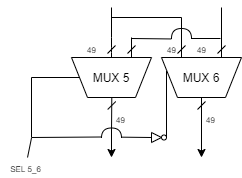
\includegraphics[scale=0.5]{mux5_6.png}
    \caption{Schema dei mux 5 e 6}
    \label{fig:mux5_6}
\end{figure}\\
La necessità di tale blocco è da ricercare nelle operazioni da eseguire, infatti dal CDFD è possibile notare che vanno eseguite rispettivamente "$\Sigma - M$" e "$M-\Sigma$", quindi il sottrattore non può avere due ingressi "inchiodati", ma deve avere la possibilità di invertire gli operandi. Un'altra possibile soluzione sarebbe potuta essere quella di mettere in uscita al sottrattore un blocchetto puramente combinatorio, con un controllo che permettesse di cambiare il segno dell'operazione a piacimento a seconda dei casi.\\
Come evidenza lo schema, i due ingressi sono sdoppiati e sono posti in ingresso ad entrambi i multiplexer, inoltre il selettore è unico e funziona in modo alternato grazie alla porta NOT. Ciò permette quindi di avere le due configurazioni richieste, "$\Sigma - M$" oppure "$M-\Sigma$".\\Un possibile miglioramento sarebbe potuto consistere nell'inserire tutta la struttura all'interno di un unico blocchetto, descrivendone il comportamento in modo behavioural e comportando così lo snellimento del data path e probabilmente una migliore implementazione da parte del compilatore che sarebbe libero di creare il blocco a suo piacimento.\\Infine il registro utilizzato ha un enable che funziona come nel caso precedente.
\subsection{Rounder}%REVISIONATO MATI+LAU
I risultati parziali, ovvero Ar', Br', Ai' e Bi' derivano solamente da operazioni di somma e sottrazione, questo quindi ha comportato l'inserimento di un mux per "convogliare" le uscite provenienti dai corrispettivi blocchi aritmetici. %PROPOSTA LAU (MEGLIO PER MATI)
Tale MUX è quindi costituito da tre ingressi, due per i dati da mandare successivamente in uscita ed un terzo posto a zero, così da evitare l'invio di dati errati ai blocchi hardware sottostanti, avendo così massimo controllo sulle uscite. Per quanto riguarda l'uscita del multiplexer, questa è un bus da 49 bit, che viene mandata in ingresso al Ruonder.\\ %mandando tutto in ingresso al Rounder su un numero adeguato di bit.\\L'uscita del multiplexer è un bus da 49 bit, il mux  stesso ha tre ingressi, due che corrispondono ai dati da mandare in uscita e il terzo messo a zero, tale scelta è stata adottata per evitare di mandare dati non corretti ai blocchi hardware sottostanti, avendo così il massimo controllo sulle uscite.
Quindi, dato che è stato scelto un Rounder con in ingresso 6 bit ed in uscita 1 bit, sono stati mandati direttamente in uscita, cioè senza passare attraverso il processo di rounding, 23 bit e di conseguenza gli ultimi 20 sono stati scartati. Tutto questo ha permesso di tornare sul formato di 24 bit richiesto dalle specifiche.\\
Il Rounder è una ROM con in ingresso un bus a 6 bit e in uscita un singolo bus da un bit, com'è stato analizzato nella sezione 4.4 del Rom Rounding.
\subsection{Splitter}%REVISIONATA MATI+LAU
Il protocollo scelto dal team prevede l'uscita dei dati in modo parallelo, quindi al primo colpo di clock escono Ar e Br e al secondo Ai e Bi, ovviamente tutti dopo il segnale di START.\\L'ordine di arrivo dei dati, che risulta essere Ar', Br', Ai', Bi', ha portato a trovare una soluzione per permetterne la corretta uscita. Com'è possibile notare, i dati sono distribuiti su quattro colpi di clock, quindi è stato necessario il salvataggio di questi prima di poterli mandare in uscita; in particolare i primi due, cioè le parti reali di A' e di B', devono uscire in concomitanza del salvataggio di Ai', così da avere al colpo di clock successivo immediatamente disponibile Bi', per mandarlo così in uscita.\\Perciò la soluzione adottata prevede due blocchi fondamentali, uno shift register e un "blocco custom" con tre ingressi e due uscite. In Figura \ref{fig:sp1} e Figura \ref{fig:sp2} sono riportati graficamente i passaggi descritti in precedenza. Qui però sono stati omessi tutti i vari segnali, come clock, sel ecc. per descrivere solamente il principio di funzionamento.\\
\begin{figure}[h]
\begin{minipage}[c]{0.5\linewidth}
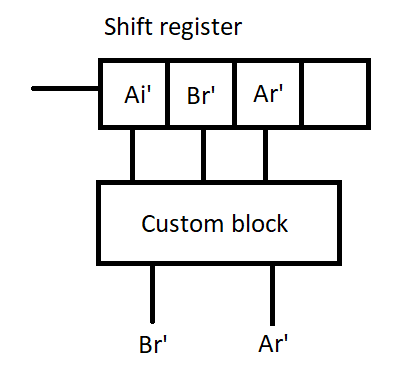
\includegraphics[scale=0.5]{slpitter1.png}
\caption{Step 1}
\label{fig:sp1}
\end{minipage}
\hspace{5mm}
 \begin{minipage}[c]{0.5\linewidth}
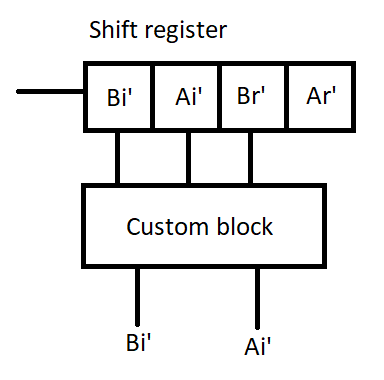
\includegraphics[scale=0.5]{slpitter2.png}
\caption{Step 2}
\label{fig:sp2}
\end{minipage} 
\end{figure}
\\
Da tali figure è possibile osservare che al colpo di clock in cui entra Ai', escono Ar' e Br', mentre, al fronte di clock successivo, il custom block seleziona e fa uscire Ai' e Bi'. \\Infine i dati vengono passati ai due registri di uscita.
\\
Inoltre lo shift register non ha nessun controllo e tale scelta è stata fatta sia per risparmiare un bit di comando, sia perché la bontà degli ingressi è assicurata dal MUX 7, che quando non smista i dati viene messo a zero.\\
Per il massimo controllo delle uscite, sono stati inseriti due registri con un output enable (il segnale è il medesimo in quanto i dati escono a coppie), il quale, se disabilitato, mette la sua uscita a "0" (ovviamente si parla sempre di un bus a 24 bit). Tale scelta è stata attuata per avere la sicurezza di non far uscire nessun dato spurio dalla butterfly. E' da sottolineare che i comandi interni alla butterfly arrivano sul fronte negativo del clock e quindi possono essere presenti alcuni istanti temporali dove esistono per mezzo periodo di clock dei dati indesiderati, basti pensare banalmente allo shift register e il custom block, che lavorano su due fasi differenti.
%\pagebreak
\section{Data path FFT 16x16}%REVISIONATA MATI+LAU
Dopo aver progettato una singola butterfly, sono state usate 32 copie di questa, per andare a costituire la struttura atta a svolgere la Fast Fourier Trasform.\\Nel caso esaminato, osservabile in Figura \ref{fig: schema FFT}, la FFT è caratterizzata da 16 ingressi, che rappresentano i campioni ricevuti, dei quali i primi 8 sono riferiti alle A, mentre i restanti alle B. Anche in uscita sono presenti 16 campioni, che rappresentano il risultato della FFT.%(CHEVVORDI'??? GIANLU G)
\\Tale struttura è composta da 4 stadi, in cui nel primo viene utilizzato un singolo gruppo di 8 butterfly, nel secondo ci sono due gruppi da 4 butterfly ciascuno, nel terzo il numero dei gruppi raddoppia, passando a 4 ciascuno da due butterfly, infine l'ultimo stadio è costituito da 8 gruppi ciascuno con una singola butterfly.
\begin{figure}[h]
    \centering
    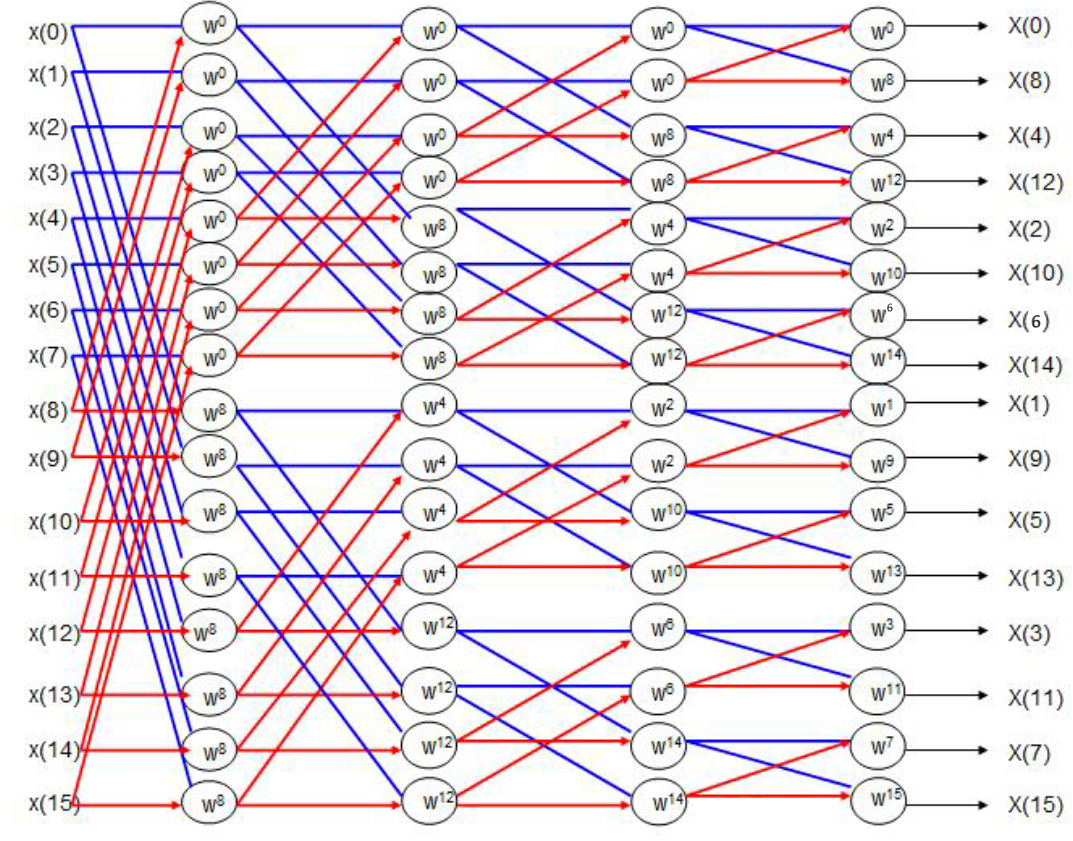
\includegraphics[scale=0.6]{FFT_scheme.png}
    \caption{FFT 16x16}
    \label{fig: schema FFT}
\end{figure}\\
Inoltre dallo schema sopra riportato è possibile notare la presenza in ogni butterfly di due termini, detti Twiddle Factors, cioè W\ap{k} e W\ap{k+N/2}, i quali assumono i seguenti valori:
\begin{itemize}
    \item $\ W\ap{k}=W\ped{r}+jW\ped{i}$, composta da una parte reale e una parte immaginaria, entrambi sulla circonferenza unitaria, quindi la loro somma in modulo deve restituire 1;
    \item $\ W\ap{k+N/2}=-W\ped{r}-jW\ped{i}$, composta anch'esso da un termine reale ed uno immaginario. E' possibile osservare che tale fattore è equivalente al precedente cambiato di segno.
\end{itemize}
Tali Twiddle Factors, diversamente dai campioni dati dall'utente, che possono variare ogni volta, sono costanti per ogni FFT, quindi il loro inserimento è demandato a una Rom cablata direttamente alla FFT, com'è possibile osservare in Figura \ref{fig: ROM W}. Tale scelta è stata ritenuta ottimale anche in ottica dell'utente finale che non dovrà preoccuparsi di apportare al sistema tutti gli 8 Twiddle Factor necessari all'FFT.
\\
\begin{figure}[h]
    \centering
    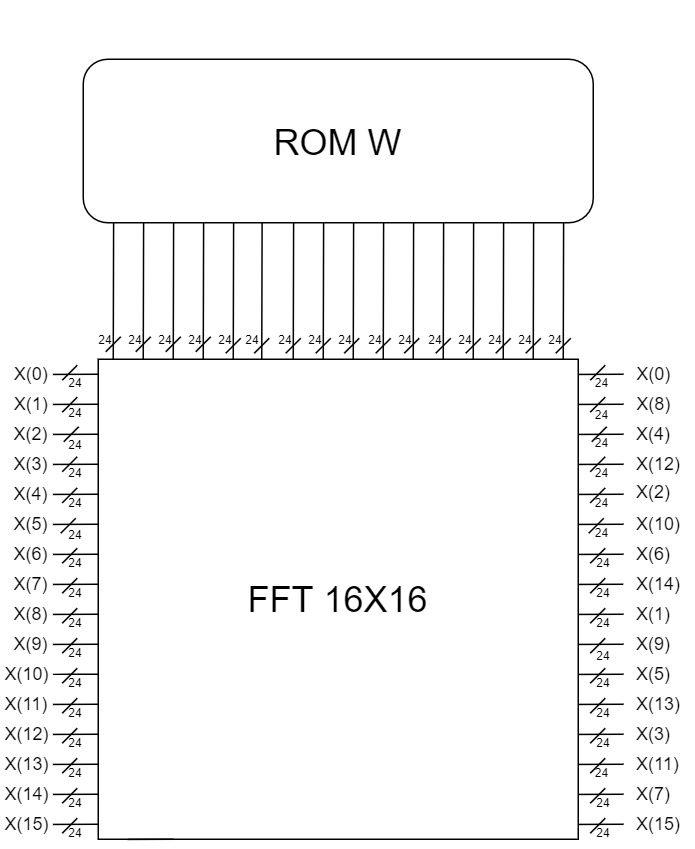
\includegraphics[scale=0.35]{ROM_W_FFT.png}
    \caption{Schema FFT con ROM W}
    \label{fig: ROM W}
\end{figure}
Ciascun W è connesso alla corrispettiva butterfly interna al blocchetto FFT.\\
%Inoltre è necessario notare che, arrivando ad ogni butterfly due W(uno l'opposto dell'altro) è sufficiente connettere ad ogni blocchetto butterfly un solo Twiddle Factor, che verrà poi semplicemente negato, per andare a rappresentare il W mancante.
%PROPOSTA DI MODIFICA (GIANLU G)\\
%Inoltre è importate notare che, arrivando ad ogni butterfly due W, che nominalmente sono diversi, ma che in realtà, data la loro natura, sono semplicemente l'uno il negato dell'altro, ciò comporta un notevole risparmio in termini di bus in quanto è necessario connettere soltanto un W (quindi un unico bus da 24 bit) dato che poi internamente la Butterfly, a seconda delle operazioni, farà in modo di negare il coefficiente.
Inoltre è importante notare che ad ogni butterfly arrivano due W nominalmente diversi, i quali però in realtà, data la loro natura, sono semplicemente l'uno il negato dell'altro. Quindi, a ragion di tale evidenza, risulta essere sufficiente la connessione di un solo Twiddle Factor ad ogni blocchetto Butterfly, che internamente, per le operazioni che lo necessitano, farà in modo di negare il coefficiente. Ciò comporta un notevole risparmio in termini di bus in quanto è impiegabile la connessione di soltanto un W, ovvero un unico bus da 24 bit, invece che due.
\\Grazie a tale tecnica è anche possibile quindi risparmiare la metà della memoria della ROM, all'interno della quale sono riportati, ciascuno su 24 bit in complemento a due, unicamente la parte reale e la parte immaginaria del Twiddle Factor W\ap{k} di ciascuna butterfly interna alla FFT. I valori utilizzati per questi sono reperibili in Tabella \ref{Twiddle Factor reale}, per quanto concerne la parte reale, ed in Tabella \ref{Twiddle Factor immaginaria}, per la parte immaginaria.
%\pagebreak
\section{Control unit}
\subsection{Timing} %REVISIONATA LAU+MATI
In Figura \ref{fig:timing_butterfly} è riportato il timing rappresentante l'esecuzione di una singola butterfly.\\
\begin{sidewaysfigure}
%\begin{figure}%[h]
    \centering
    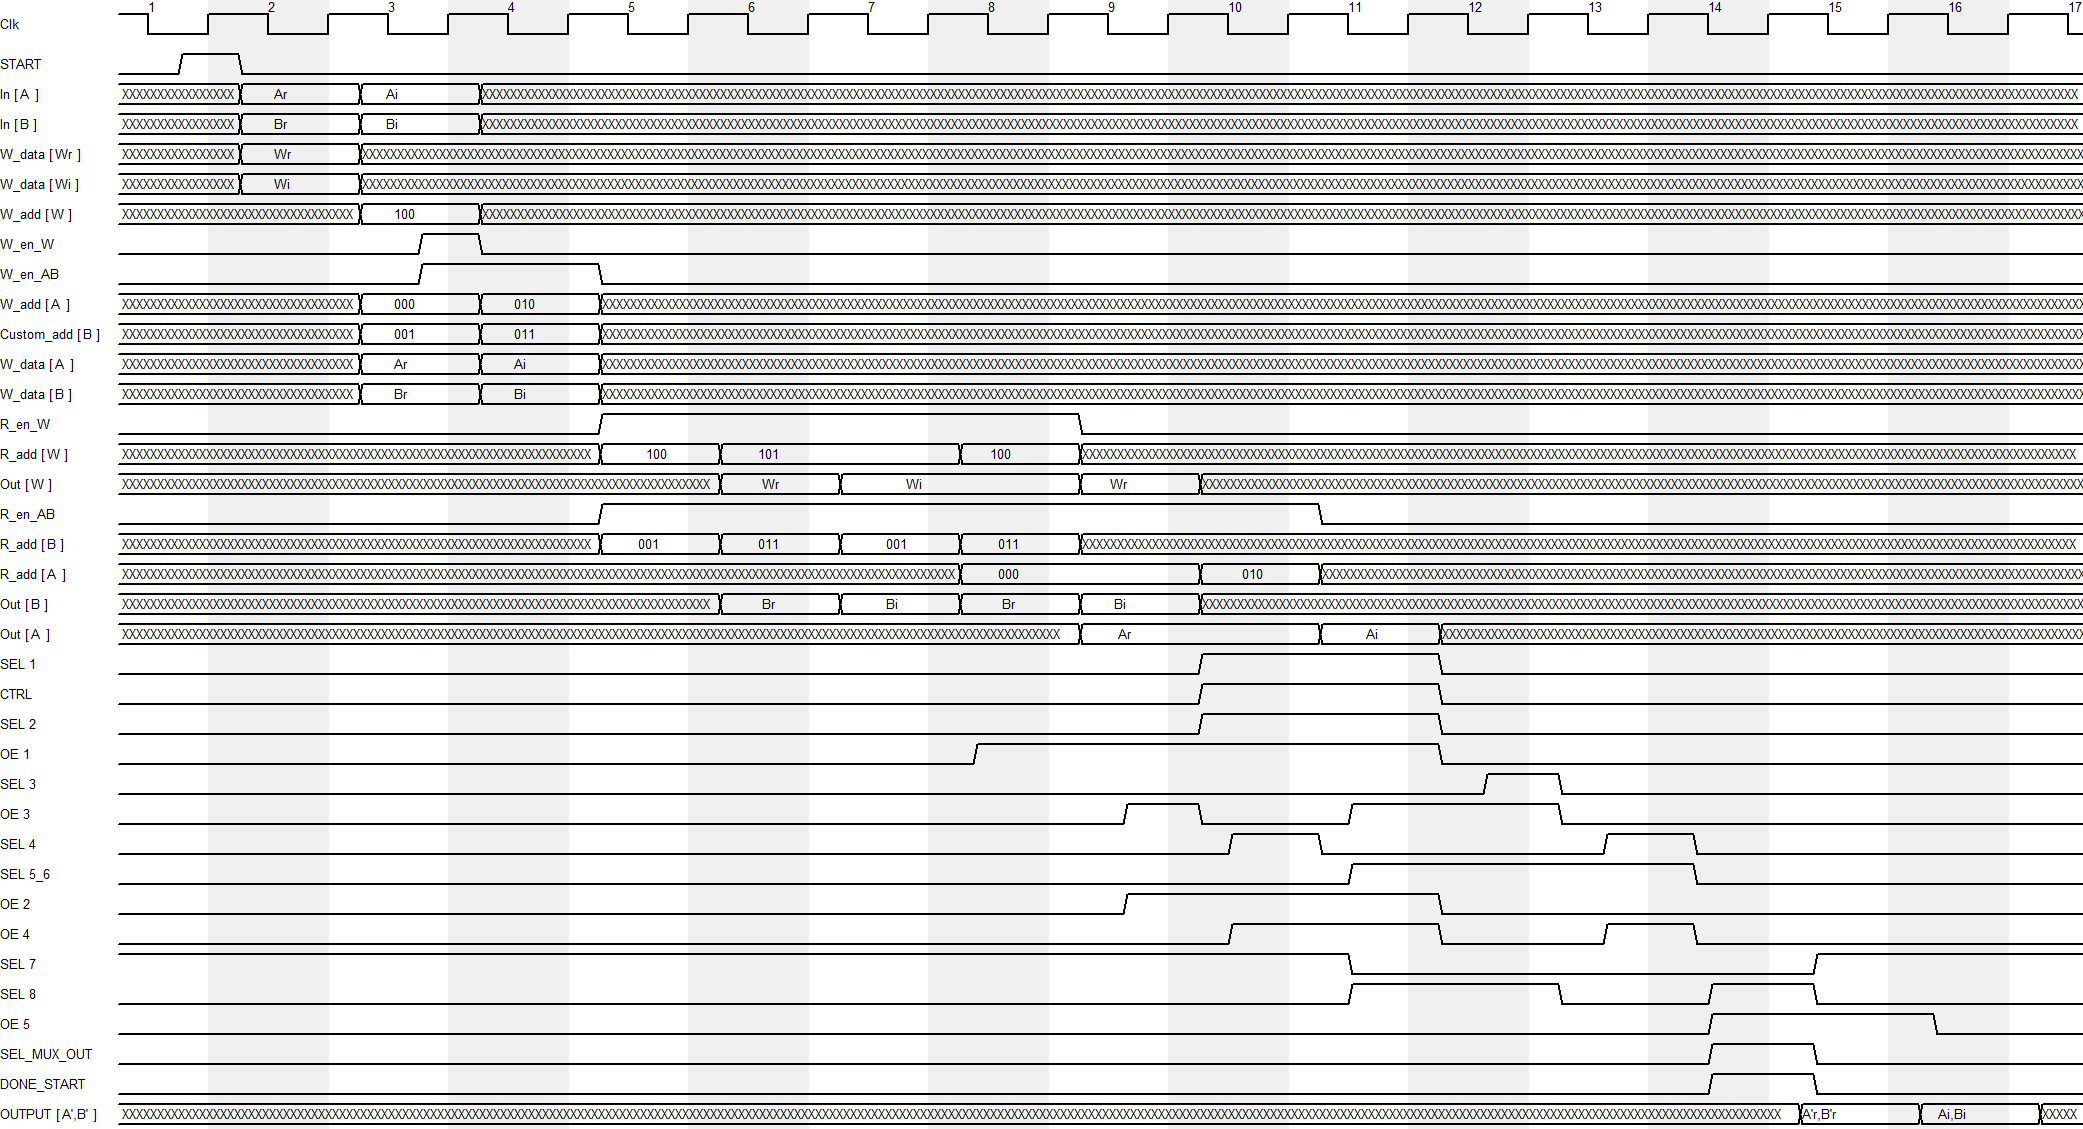
\includegraphics[scale=0.43]{timing_butterfly.png}
    \caption{Timing}
    \label{fig:timing_butterfly}
%\end{figure}
\end{sidewaysfigure}\\
\newpage
Si è voluto porre l'attenzione su alcuni aspetti salienti per comprenderne in modo più agevole il procedimento:
\begin{itemize}
    \item SEL 1: è riferito al MUX\_1, posto in corrispondenza di uno dei due ingressi del moltiplicatore.\\Per tale controllo è stato scelto di porre il bus a '0' sia nel caso di 'DON'T CARE' che di selezione dell'ingresso 'B', mentre è stato impostato '1' come comando per selezionare l'ingresso 'A';
    \item CTRL: seleziona quale tipo di moltiplicazione svolgere. Quando viene effettuato lo 'shift', cioè la moltiplicazione per due, è stato impostato il bus a '1', mentre per il caso di moltiplicazione 'classica' (Y*Z) o di 'DON'T CARE' il bus è a '0';
    \item SEL 2: controlla il MUX\_2 ed è ad '1' quando riceve dal moltiplicatore il risultato dello shift. Invece risulta essere a '0' quando gli arriva in ingresso la moltiplicazione 'classica' od è nello stato di 'DON'T CARE';
    \item SEL 3: gestisce il MUX\_3, posto ad uno degli ingressi del sommatore. Mediante questo viene selezionata l'opzione 'A' o 'DON'T CARE' se il bus è a zero, mentre se è ad '1' in ingresso entra il risultato della sommatoria svolta precedentemente;
    \item SEL 4: riferito al MUX\_4, è posto ad '1' quando è selezionato il risultato della sommatoria, ed è a '0' nel caso che in ingresso sia stato scelto di avere il risultato della sottrazione o ci sia la condizione di 'DON'T CARE';
    \item SEL 5\_6: è il controllo di un blocco all'ingresso del quale sono presenti l'uscita del MUX\_4 e il risultato della moltiplicazione se il bus è posto a '0', mentre tali ingressi sono invertiti di posizione nel caso il bus sia ad '1'. Anche in questo caso, come nei precedenti, se il bus è nello stato di 'DON'T CARE', è a zero;
    \item SEL 7 e SEL 8: fanno riferimento al MUX\_7, posizionato antecedentemente al Rounder. Qui è stata necessaria una codifica con due bit, di cui il primo è SEL 7 ed il secondo SEL 8. Quindi ci sarà '01' quando viene selezionato il risultato della sottrazione, mentre '00' quando deve entrare il risultato della sommatoria, in tutti gli altri casi il Mux manda in uscita zero, così da evitare di ritrovare in uscita dati non voluti, tagliando fuori la parte aritmetica;
    \item SEL\_DEMUX: è a '0' quando seleziona A\ped{r}' e B\ped{r}' o nello stato di 'DON'T CARE'. Per la selezione di A\ped{i}' e B\ped{i}' invece il bus è posto ad '1'.
\end{itemize} 
\subsection{Diagramma di stato}%REVISIONATO MATI+LAU
In figura \ref{fig:pallogramma} è riportato il diagramma di stato progettato per la Butterfly.
\begin{figure}[h]
    \centering
    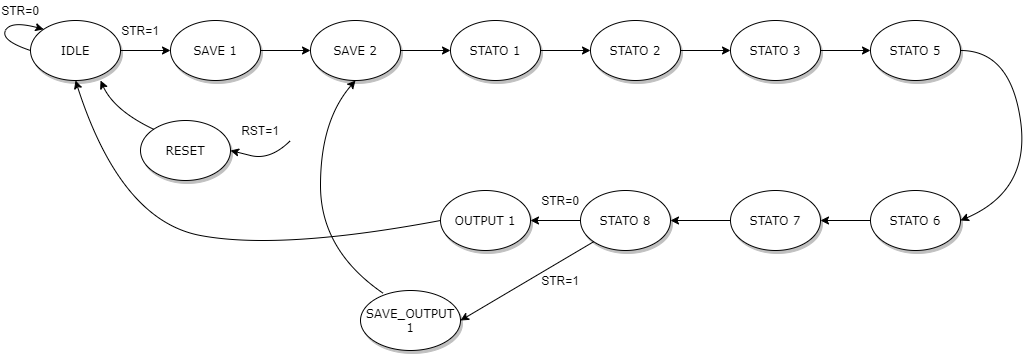
\includegraphics[scale=0.4]{Pallogramma.png}
    \caption{Diagramma di stato}
    \label{fig:pallogramma}
\end{figure}\\
\newpage
In tale progetto è stata adottata la tecnica del "salto a due vie" abbinata alla STATUS PLA, che è semplicemente una ROM capace di modificare il comportamento della CU in base al verificarsi di alcune condizioni, le quali indicano se la progressione nello stato successivo debba essere in sequenza o tramite un salto.\\
La codifica utilizzata per la selezione del salto o della sequenza sono state:
\begin{itemize}
    \item "1"= SALTO
    \item "0"= SEQUENZA
\end{itemize}
In Tabella \ref{tab:statuspla} è osservabile la codifica di tale PLA. Inoltre è stato necessario l'inserimento di due bit di Condition Code Validation, così da avere uno spazio delle soluzioni possibili molto ampio. In particolare, è possibile decidere tra salti condizionati dal segnale di start, salti incondizionati e la semplice sequenza.\\Inizialmente è stato usato un singolo bit di CC, ma tale scelta è risultata poi inefficace e quindi è stato optato per una soluzione con 2 bit di CC.\\Uno dei passaggi critici è risultato essere l'evoluzione da IDLE a START, poiché l'address alla STATUS PLA deve necessariamente avere un codice contiguo, ovvero un numero su cui differisca solo LSB così da progredire in sequenza, mentre il salto permette di rimanere in IDLE finchè non arriva il segnale di START. Sono stati scelti "00" e "01", dove l' "1" è fornito dallo start che viene applicato dall'esterno.\\Altro punto cruciale è rappresentato dallo "sdoppiamento" del pallogramma, ovvero il punto il cui il sistema è capace di sentire un nuovo START e quindi di iniziare una nuova elaborazione. In tal punto, come nel precedente caso, la necessità di sentire uno start ha dettato l'uso di due address consecutivi, i quali però devono obbligatoriamente differire dai due indicati prima, in quanto se ci fosse per esempio "00" il sistema ritornerebbe nello stato di IDLE. Quindi le uniche scelte disponibili sono state "10" ed "11". Tale soluzione però non è risultata capace di coprire il caso possibile di salto incondizionato, non garantendo così la possibilità di chiudere l'evoluzione degli stati e tornare in IDLE oppure andare nuovamente in uno stato intermedio per continuare una nuova esecuzione. 
\noindent Quindi è stata adottata la soluzione con due bit, andando così a garantire un maggior controllo, permettendo anche di eseguire i salti incondizionati.\\in Tabella \ref{tab:statuspla} sono riportate tutte le codifiche della ROM.\\
%%%%%%%%%%%%%%%%%%%%%%%%%%
\begin{longtable}{*4c}
\caption{Codifica della Status Pla}\label{tab:statuspla}\\
\toprule
CC(1) & CC(0) & STR & JMP/SEQ\\
\midrule
\endfirsthead
CC(1) & CC(0) & STR &JMP/SEQ\\
\midrule
\endhead
\midrule
\endfoot
\bottomrule
\endlastfoot
0 & 0 & 0 & JMP\\
0 & 0 & 1 & SEQ\\
0 & 1 & 0 & JMP\\
0 & 1 & 1 & JMP\\
1 & 0 & 0 & SEQ\\
1 & 0 & 1 & SEQ\\
1 & 1 & 0 & JMP\\
1 & 1 & 1 & JMP\\

\end{longtable}
%%%%%%%%%%%%%%%%%%%%%%%%%%%
Dalla tabella è possibile notare che, se il sistema non sente lo START salta e torna in IDLE, invece se lo percepisce va in sequenza iniziando tutta la progressione degli stati. Per mantenere la coerenza con quello fatto in precedenza, è stata utilizzata la stessa tecnica anche con la modalità "full speed", ovvero nello STATO 8 il sistema è capace di sentire un nuovo "START", se lo riceve va in sequenza ,finendo in "SAVE\textunderscore OUTPUT 1", se non lo sente salta in "OUTPUT 1", richiudendosi poi in "IDLE". L'adozione di questa soluzione ha comportato il riempimento della ROM in modo leggermente differente, dopo il campo riferito allo "STATO 8" è stato inserito il campo "SAVE\textunderscore OUTPUT 1" e lo stato "OUTPUT 1" nella zona di ROM adibita ai salti, ovvero la parte finale. I salti incondizionati sono stati gestiti ponendo i CC=11. \\
La presenza di un solo stato "output" non deve stupire in quanto i primi due dati  vengono mandati in uscita sui registri di interfacciamento allo stato "OUTPUT 1" e "SAVE\textunderscore OUTPUT 1". Poi, al colpo di clock successivo, escono gli altri due ed il sistema deve mandare a livello logico basso l'output enable dei due registri. Ciò, come si può notare dal timing diagram, corrisponde ai comandi dati nello stato di "IDLE", usato qui per risparmiare uno stato.\\Per quanto riguarda invece lo stato "SAVE\textunderscore OUTPUT 1", in questo, oltre a provvedere all'uscita dei primi due dati, viene creata anche la situazione adeguata per il salvataggio dei primi due ingressi, attivando il "Write enable" del Register File e ponendo  gli address corretti. Dopodiché il sistema evolve nello stato "SAVE 2", che viene sfruttato per abbassare l'output enable dei due registri di uscita e per dare i comandi di salvataggio della seconda coppia di dati.
\\N.B. Notare che sono state omesse tutte le connessioni tra i vari stati ed il RESET, così da migliorare la comprensione del diagramma, ovviamente, per come è stata progettata la Control Unit, da ogni stato è possibile passare allo stato di RESET, come sarà descritto meglio nelle prossime sezioni.
%%%%%%%%%%%%%%%%%%%%ù
\subsection{Struttura della Control Unit}
%REVISIONATO GIANLU+MATI+LAU
Per la Control Unit, rappresentante il cuore pulsante di tutto il progetto, è stata adottata una soluzione il più generale e semplice possibile, con una struttura con indirizzamento implicito, limitando i salti possibili solamente a "due vie", sfruttando la STATUS PLA. Lo schema concettuale comprendente tutti i blocchi ed è riportato in Figura \ref{fig:cu}.\\Notare che lo schema fornito è puramente di principio e che per ulteriori informazioni è necessario fare riferimento ai file VHDL riportati nella Sezione 10.
\begin{figure}[h]
    \centering
    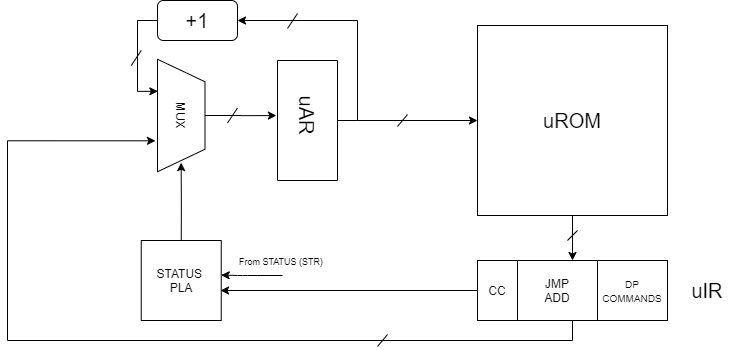
\includegraphics[scale=0.5]{controlunit.png}
    \caption{Struttura Control Unit}
    \label{fig:cu}
\end{figure}
\\Come è noto da teoria, tale struttura ad indirizzamento implicito permette di implementare una control unit attraverso una struttura ben definita, precisa e standard, agevolando il progettista nel processo di sviluppo del progetto in quanto eventuali modifiche vanno a riflettersi solamente sulla variazione dei campi della $\mu$ROM, a differenza di altre soluzioni dove il comportamento del sistema è cablato direttamente e intrinsecamente nella struttura stessa della Control Unit.\\
Il comportamento è molto semplice: la sequenza degli stati è garantita da un incrementatore, che prende il valore attuale del $\mu$Address Register e lo aumenta di uno, reinserendolo in ingresso e fornendo così il "next state", mentre il "current state" in uscita dal $\mu$AR viene posto ingresso alla $\mu$ROM, che estrae tutto il necessario per lo stato in questione. Poi tutto ciò viene inserito nel $\mu$Instruction Register.\\E' da porre attenzione al fatto che nella soluzione adottata, il CC, la ROM del Command Generator e la ROM, che estrae il Jump Address, sono state "fuse" in un solo blocco di memoria, inserendo i campi appositi. Inoltre la gestione dei salti è realizzata in modo elementare: il campo CC arriva come ingresso alla STATUS PLA e seleziona o meno una condizione di salto, sarà poi il segnale di stato selezionato a determinare l'uscita della PLA, che girerà il mux per prendere il "next state" derivante dall'incrementatore oppure quello del "jump address".\\
Il reset è gestito in maniera estremamente semplice, ovvero una volta giunto dall'esterno, questo va a resettare il $\mu AR$, che punta a sua volta alla prima locazione della $\mu ROM$ dove è codificato lo stato di "RESET".\\ E' chiaro che l'assegnazione dei comandi e del CC deve avvenire in un arco temporale che rientri nell'intervallo tra un colpo di clock e il successivo. Tale fattore ha comportato quindi la necessità di sfruttare la fase negativa del clock. Infatti, il $\mu IR$, com'è possibile notare dai file VHDL, è sensibile al fronte negativo. Questo permette anche un'immediata diffusione del reset nel sistema, in quanto, appena il $\mu$AR viene resettato, anche tutto il sistema è resettato sul fronte negativo e l'intervallo temporale tra questi due istanti è molto breve. \\
Dopo la stesura del diagramma di si è dimensionato il numero di bit necessario alla codifica degli stati, il quale è stato scelto pari a n=4 bit, un numero più che adeguato per codificare tutti i 13 stati.
\subsection{Contenuto della $\mu$Rom}%REVISIONATA MATI
Il centro nevralgico del sistema risiede all'interno del contenuto dei campi della $\mu$ROM, che viene passato al $\mu$IR. Poi attraverso questo registro ogni campo viene smistato verso la propria destinazione.\\La $\mu$ROM, costituita tutta da righe di dimensioni di 41 bit ciascuna, è stata costruita secondo la struttura presente in Tabella \ref{tab:Struttura microROM}. Ponendo attenzione su questa, è possibile osservare che a partire dall'MSB sono presenti due bit di CC, poi 4 bit di jump address e infine 41 bit di comandi.\\\\
%\begin{tiny}
%\centering
\begin{longtable}{*5c}
%\footnotesize
\caption{Struttura $\mu$ROM}
\label{tab:Struttura microROM}\\
\toprule
 Stato & CC & \thead{Jump\\Address} & \thead{Bit di\\comando} & Codifica \\
\midrule
\endfirsthead
 Stato & CC & \thead{Jump\\Address} & \thead{Bit di\\comando} & Codifica \\
\midrule
\endhead
\midrule
\endfoot
\bottomrule
\endlastfoot
RESET &	10 & 0001 &	01000000000000000000000000000001010 &00000\\
IDLE  &	00 & 0001 & 01000000000000000000000000000001000	&00001\\
SAVE1 & 10 & 0001 &	01001101000000000000000000000001000	&00010\\
SAVE2 & 10 & 0001 &	01000001000000000000000000000001000	&00011\\
SAVE3 & 10 & 0001 & 01000000001100100000100000000001000 &00100\\
SAVE4 & 10 & 0001 &	01000000001101100001100000000001000 &00101\\
STATO1 & 10	& 0001 & 01000000001101100000100000000001000 &00110\\
STATO2 & 10	& 0001 & 01000000001100100001100010000001000 &00111\\
STATO3 & 10	& 0001 & 01000000000000100000000010100101000 &01000\\
STATO4 & 10	& 0001 & 01000000000000101000011110010111000 &01001\\
STATO5 & 10	& 0001 & 00000000000000000000011110101111000 &01010\\
STATO6 & 10	& 0001 & 00000000000000000000000001101001000 &01011\\
STATO7 & 10	& 0001 & 00000000000000000000000000011010000 &01100\\
STATO8 & 00 & 1111 & 00100000000000000000000000000001101 &01101\\
SAVE1\_OUTPUT1 & 11	& 0011 & 01001101000000000000000000000001100 &01110\\
OUTPUT1&11&0001&01000000000000000000000000000001100&01111\\
%\normalsize
\end{longtable}
%\end{tiny}
%\end{sidewaystable}
%\newpage 
\noindent \\Il  significato di ogni bit è riportato nella Tabella \ref{tab:Contenuto microROM}. In qeusta è stato inserito anche l'ordine con cui sono stati assegnati i bit di comando al segnale che raggiunge il datapath (dp\textunderscore commands \textunderscore sig).
%\begin{small}
\begin{longtable}{*3c}
\caption{Contenuto $\mu$ROM}
\label{tab:Contenuto microROM}\\
\toprule
Comando & $\mu$ROM(n) & dp\_commands\_sig(n)\\
\midrule
\endfirsthead
Comando &  $\mu$ROM(n) & dp\_commands\_sig(n)\\
\midrule
\endhead
\midrule
\endfoot
\bottomrule
\endlastfoot
Done & 0 & - \\ 
Reset & 1 & 0 \\
OE5 & 2 & 1  \\
SEL7 & 3 & 2  \\
OE4 & 4 & 3 \\
OE2 & 5 & 4 \\
SEL5-6 & 6 & 5 \\
SEL4 & 7 & 6 \\
OE3 & 8 & 7 \\
SEL3 & 9 & 8 \\
OE1 & 10 & 9 \\
SEL2 & 11 & 10 \\
CTRL & 12 & 11 \\
SEL1 & 13 & 12 \\
R\_{addB} & 14,15,16 & 13,14,15 \\
R\_{addA} & 17,18,19 & 16,17,18 \\
R\_{enAB} & 20 & 19 \\
R\_{addW} & 21,22,23 & 20,21,22 \\
R\_{enW} & 24 & 23 \\
W\_{addA} & 25,26,27 & 24,25,26 \\
W\_{enAB} & 28 & 27 \\
W\_{addW} & 29,30,31 & 28,29,30 \\
W\_{enW} & 32 & 31 \\
Sel Demux & 33 & 32\\
SEL8 & 34 & 33\\
jmp(0) & 35 & -\\
jmp(1) & 36 & -\\
jmp(2) & 37 & -\\
jmp(3) & 38 & -\\
CC(LSB) & 39 & -\\
CC(MSB) & 40 & -\\
\end{longtable}
%\end{small}
\newpage
\section{Test} %REVISIONATA LAU+MATI
Al fine di verificare la bontà del sistema FFT sviluppato, sono stati utilizzati dei vettori di test forniti dal Docente, i quali sono stati testati mediante Modelsim, sia in modalità singola, sia in modalità "full speed", per la quale sono stati tenuti in considerazione 3 start.\\Tali test comprendono un'ampia gamma di tipologie, tra cui: sinusoide, Delta di Dirac, segnale costante, segnale rettangolare ed altri.\\Il numero totale di test svolti equivale a 6 ed è comprensivo anche di uscite con termini immaginari, coprendo così una vasta casistica di possibili trasformate.\\I valori forniti come test sono dei numeri interi che, ovviamente, fuoriescono dalla dinamica fractional point (-1 < Dinamic < +1), quindi è stato necessario inserire i giusti valori in ingresso alla FFT, mediante l'utilizzo di 5 bit di guardia, che hanno permesso la riduzione dei dati in ingresso, portandoli ad essere in modulo minori di $\dfrac{1}{2^5}$, ovvero minori di circa 0,031. Il file VHDL "fft\textunderscore test \textunderscore v2" contine tutti i test effettuati, per eseguire i vari test l'utente non deve fare altro che "scommentare" le parti corrispondenti.
%\subsection{Software Matlab}
%CHE SI FA SI METTE IL PROGRAMMEGA CHE HO FATTO?
%\\ SE SI, VANNO MESSI ANCHE I RISULTATI DI MATLAB SENNò NON %HA SENSO
\subsection{Delta di Dirac}
Il vettore di test fornito consisteva in una Delta di Dirac di ampiezza A=1, quindi per il test è stato scelto un valore pari a A'=0,01, in modo che rientrasse perfettamente nel formato di dati richiesto.\\Dato che il sistema lavora senza l'utilizzo di una libreria che gestisce il formato fractional point, è stato necessario scalare tale numero in base al fattore di scala (sf) adottato, che nel caso in questione equivale a sf=$2^k$, con k=23; quindi il valore ottenuto è x$_{n=0}=A'*2^k=83886$.\\ Dopo aver codificato in complemento a due (C2) tale cifra, questa è stata passata come input alla FFT.\\Di seguito sono riportati gli ingressi e le uscite di questo test:
\begin{itemize}
    \item Ingresso: x[n]=[1,0,0,0,0,0,0,0,0,0,0,0,0,0,0,0]
    \item Uscita:   X[k]=[1,1,1,1,1,1,1,1,1,1,1,1,1,1,1,1]
\end{itemize}
Di seguito si riportano i risultati del test.
\begin{figure}[h]
    \centering
    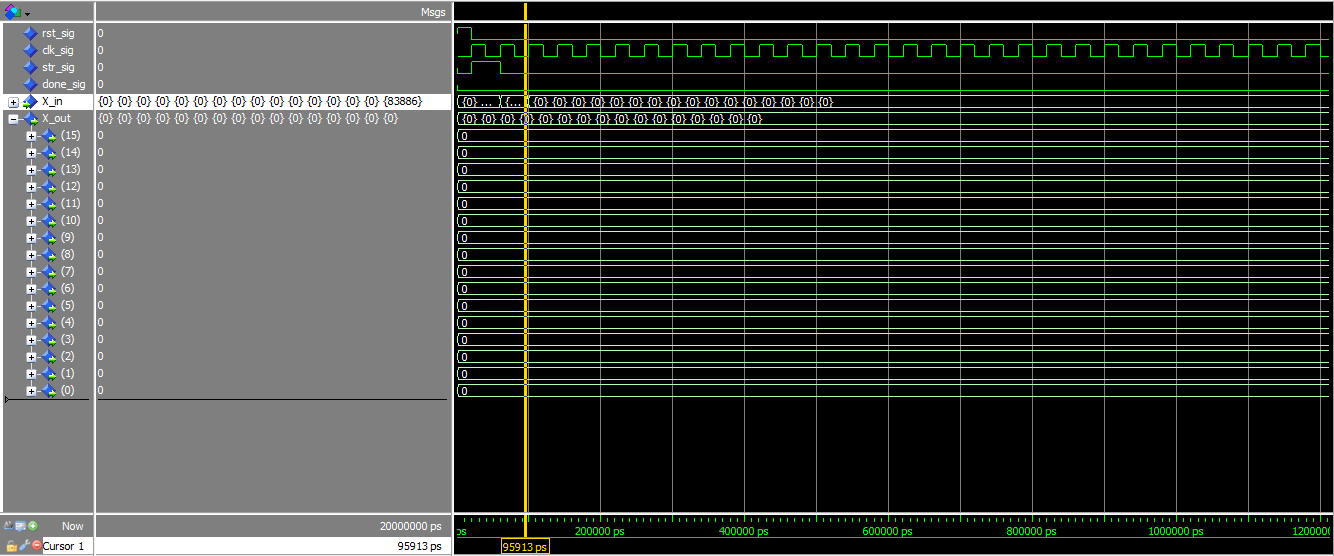
\includegraphics[scale=0.45]{test_delta/fs_delta_in.png}
    \caption{Delta di Dirac: dati in ingresso}
    \label{fig:delta_in}
\end{figure}\\
\noindent Dalla Figura \ref{fig:delta_in} è possibile osservare che dopo lo Start viene passato il vettore di ingresso, di cui è presente il valore a sinistra della progressione dei segnali. Inoltre è da notare che l'LSB, ovvero x[0], è l'elemento più a destra.
\pagebreak
\begin{figure}[h]
    \centering
    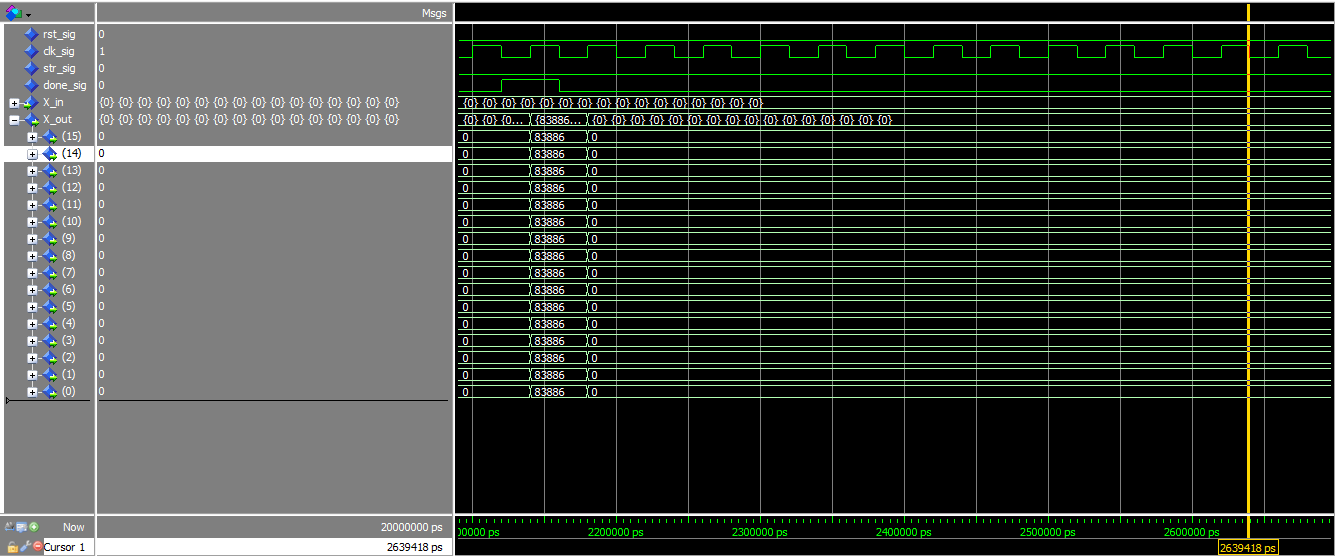
\includegraphics[scale=0.45]{test_delta/fs_delta_out.png}
    \caption{Delta di Dirac: dati in uscita}
    \label{fig:delta_out}
\end{figure}\\
In Figura \ref{fig:delta_out} è importante porre attenzione alle uscite, che hanno tutte il valore di 83886, che corrisponde ad X[k]=0.01, il che è congruo con il risultato atteso.\\
\begin{figure}[h]
    \centering
    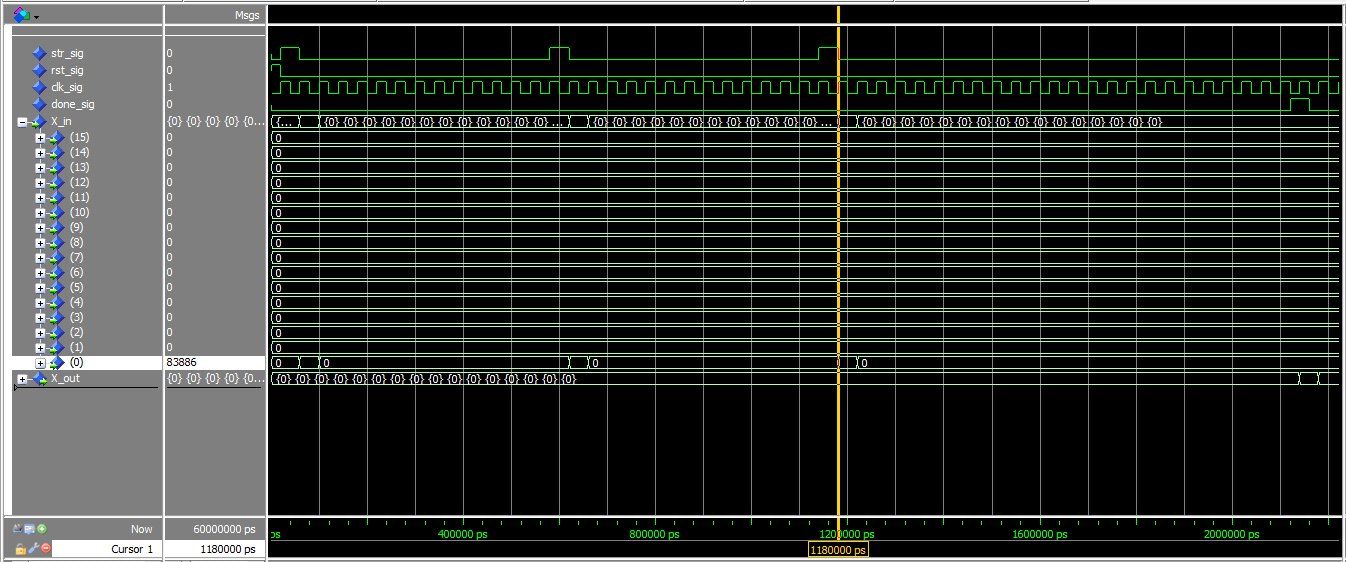
\includegraphics[scale=0.45]{test_delta/fs_delta_in_double.png}
    \caption{Delta di Dirac: dati in ingresso "full speed"}
    \label{fig:delta_full}
\end{figure}\\
In Figura \ref{fig:delta_full} è riportata la modalità "full speed" con i vari Start dati dopo 13 colpi di clock e i conseguenti inserimenti degli ingressi.\\
Per i valori numerici consultare la Tabella \ref{tab:delta}
\pagebreak
\begin{figure}[h]
    \centering
    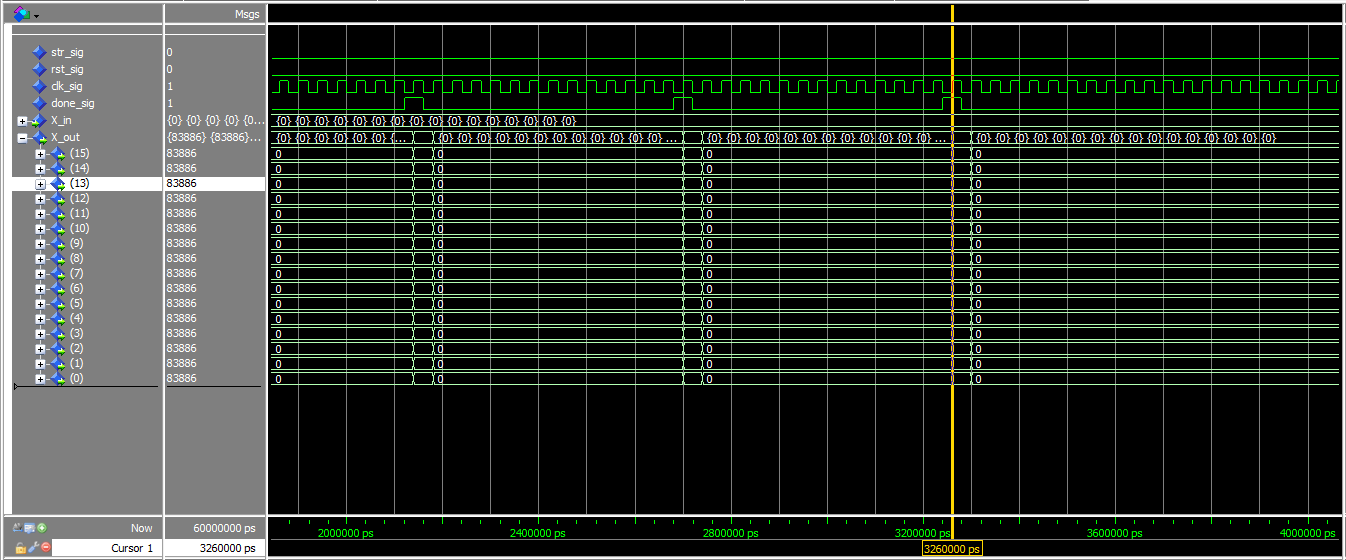
\includegraphics[scale=0.45]{test_delta/fs_delta_out_double.png}
    \caption{Delta di Dirac: dati in uscita "full speed"}
    \label{fig:delta_full_out}
\end{figure}\\
In Figura \ref{fig:delta_full_out} è presente la doppia uscita derivante dalla modalità "full speed".\\Da tale immagine è possibile osservare che, ovviamente, i risultati ottenuti sono i medesimi. Per aiutare a studiare meglio la simulazione riportata, è stato posto un marker sull'uscita della terza chiamata di FFT.\\
In Tabella \ref{tab:delta} sono disponibili tutti i dati in formato numerico.
\subsection{Segnale costante}
Questo test è focalizzato su un'altra trasformata notevole, ovvero quella del segnale costante, che nel dominio della frequenza corrisponde a una Delta di Dirac, ovvero il duale del caso precedente.Sono stati utilizzati i medesimi valori numerici.\\La presentazione dei dati è identica al caso precedente ed inizia con il riportare di seguito gli ingressi e le uscite di questo test:
\begin{itemize}
    \item Ingresso: x[n]=[-1,-1,-1,-1,-1,-1,-1,-1,-1,-1,-1,-1,-1,-1,-1,-1]
    \item Uscita:   X[k]=[16,0,0,0,0,0,0,0,0,0,0,0,0,0,0]
\end{itemize}
Successivamente sono presenti i risultati del test:
\begin{figure}[h]
    \centering
    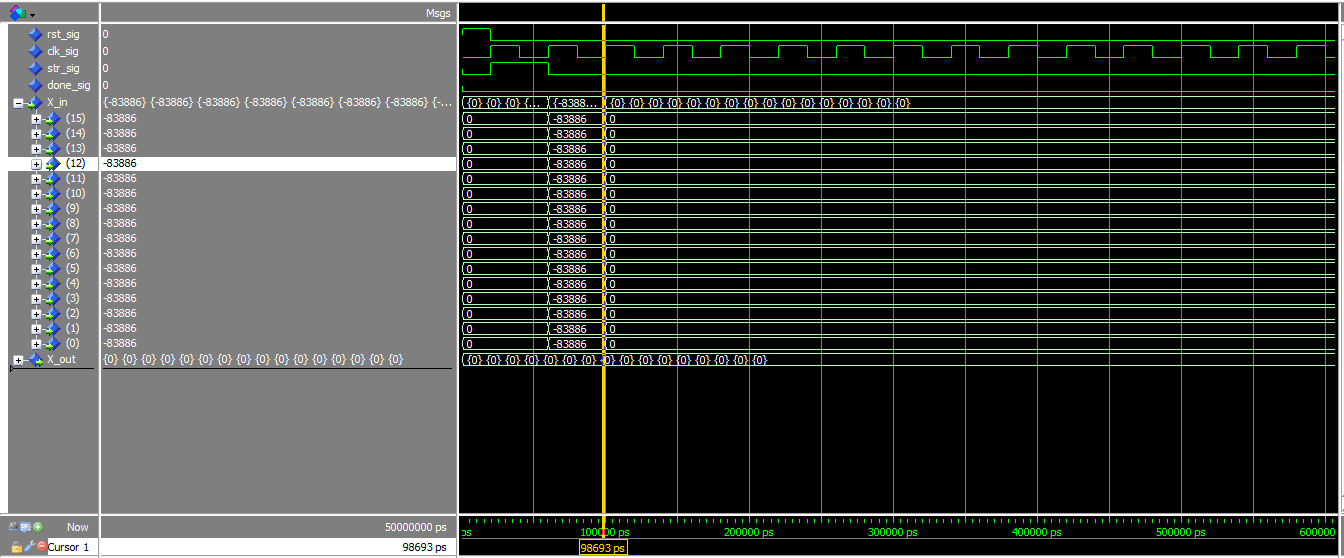
\includegraphics[scale=0.45]{test_const(-1)/fs_cost(-1)_in.png}
    \caption{Segnale costante: dati in uscita "full speed"}
    \label{fig:const_in}
\end{figure}\\
Dalla Figura \ref{fig:const_in} è osservabile che il vettore in ingresso ha un valore, come nel caso precedente, pari a x$_{in}$=-83886, ovvero x$_{in}$=-0,01.
\pagebreak
\begin{figure}[h]
    \centering
    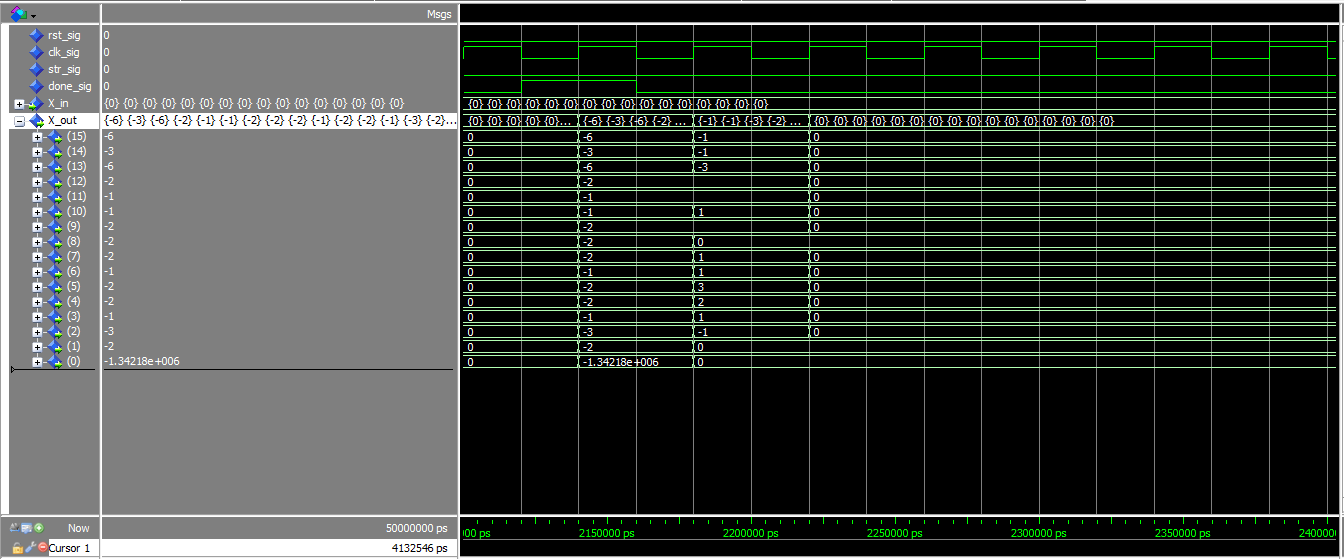
\includegraphics[scale=0.45]{test_const(-1)/fs_cost(-1)_out.png}
    \caption{Segnale costante: dati in uscita }
    \label{fig:const_out}
\end{figure}\\
In Figura \ref{fig:const_out} sono presenti le uscite dopo il segnale di "DONE". Il valore in posizione zero è pari a X[0]=$-1.34218*10^6$, il quale, convertito con lo scale factor, viene trasformato in X[0]=-0,16 , che è concorde con il risultato atteso. Gli altri campioni, sia parte reale che immaginaria, non sono esattamente zero e ciò è conseguenza del fatto che le operazioni subiscono degli arrotondamenti e che inoltre per il formato utilizzato per rappresentare i Twiddle Factor (formato fractional point complemento a due) il massimo numero positivo rappresentabile è 8388607, corrispondente a 0,9999998808, e quindi la presenza di W$_0$=1 crea dei risultati inattesi, non assumendo tale esatto valore. Un'analisi più approfondita ha portato a dire che però tali uscite sono trascurabili in quanto rappresentano un numero molto piccolo, dell'ordine di $10^{-6}$, e quindi l'errore commesso è reputato più che accettabile rispetto all'uscita desiderata, pari a zero.
\begin{figure}[h]
    \centering
    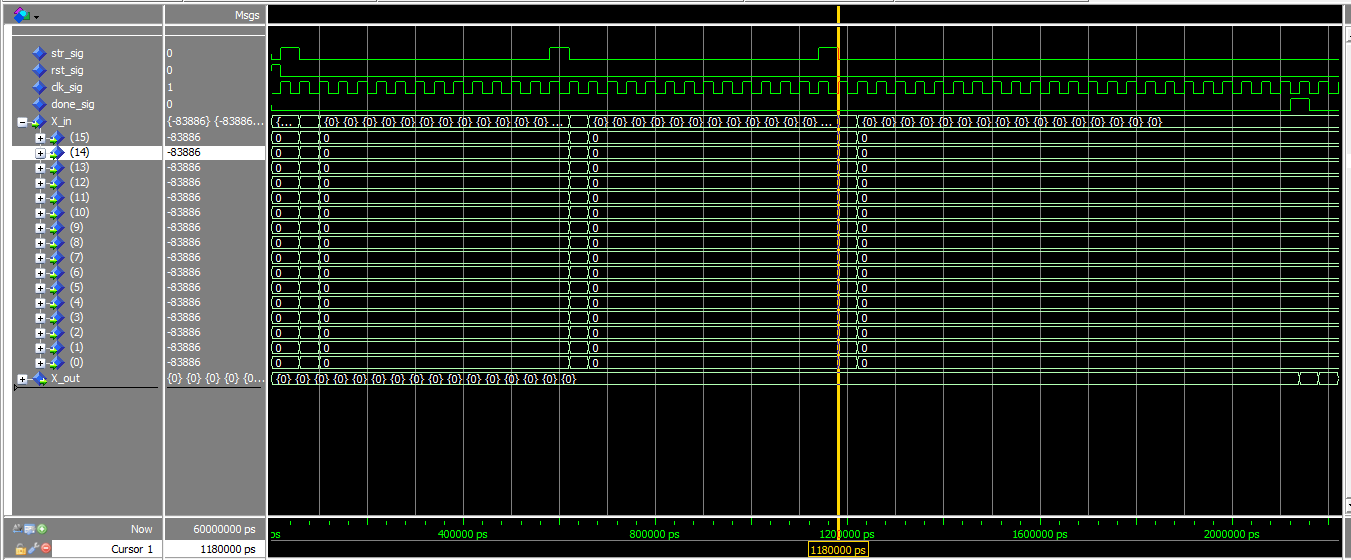
\includegraphics[scale=0.45]{test_const(-1)/fs_cost(-1)_in_double.png}
    \caption{Segnale costante: dati in ingresso "full speed"}
    \label{fig:const_in_doble}
\end{figure}\\
In Figura \ref{fig:const_in_doble} è osservabile l'inserimento dei dati in modalità full speed. Qui il valore del vettore di ingresso è visibile a sinistra nella finestra "Waves" di Modelsim.
\pagebreak
\begin{figure}[h]
    \centering
    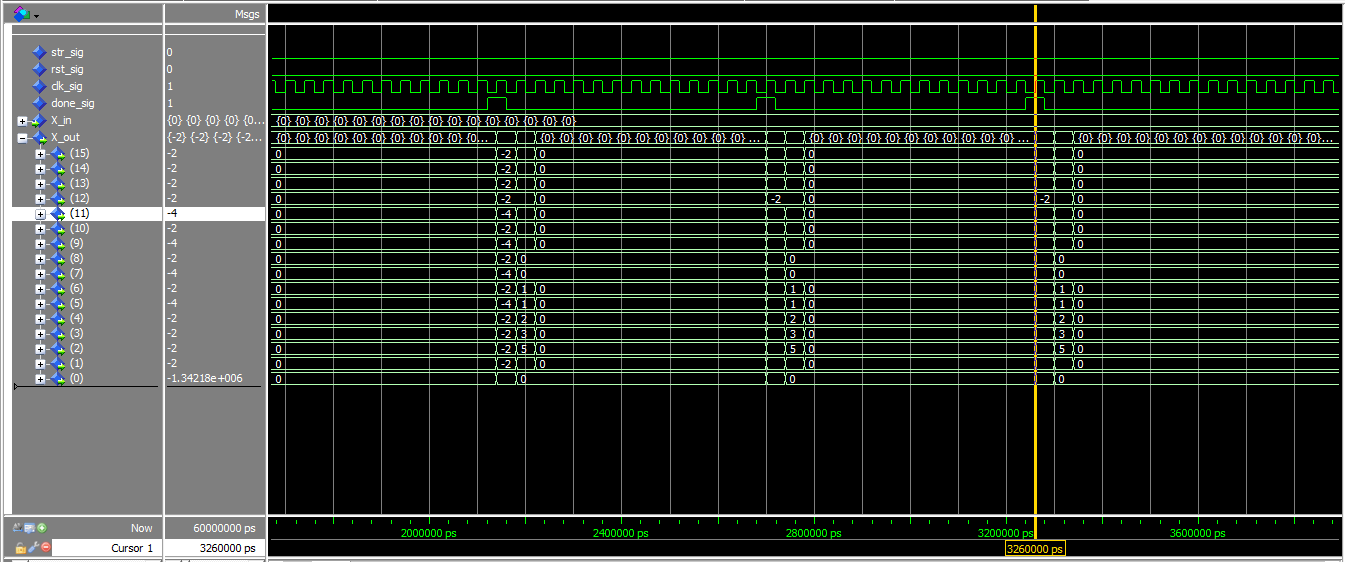
\includegraphics[scale=0.45]{test_const(-1)/fs_cost(-1)_out_double.png}
    \caption{Segnale costante: dati in uscita "full speed"}
    \label{fig:const_out_doble}
\end{figure}\\
In Figura \ref{fig:const_out_doble} sono presenti le uscite delle tre FFT consecutive.\\Ognuna di queste è data al colpo di clock successivo al segnale di "DONE". Il marker è stato posto solamente sulle uscite reali; per vedere tutti i valori è possibile fare testo alla Tabella al sottocapitolo \ref{tab:const}
%%%%%%%%%%%%%%%%%%%%%%%%%%%%%%%%
\subsection{Sinusoide}
In questo test come vettore di ingresso è stato utilizzato una sinusoide di ampiezza A=1, la cui trasformata di Fourier è una Delta di Dirac centrata alla frequenza della sinusoide. I valori numerici sono i medesimi dei casi precedenti, infatti è stato utilizzato A'=83886 pari a 0,01.\\Di seguito sono riportati gli ingressi e le uscite di tale test:
\begin{itemize}
    \item Ingresso: x[n]=[-1,0,1,0,-1,0,1,0,-1,0,1,0,-1,0,1,0]
    \item Uscita:   X[k]=[0,0,0,0,-8,0,0,0,0,0,0,0,-8,0,0,0]
\end{itemize}
Già dal vettore di uscita è evidente la caratteristica della FFT di ribaltare la parte di spettro simmetrico delle "frequenze negative" nella parte positiva di questo.\\Di seguito si riportano i risultati del test:
\begin{figure}[h]
    \centering
    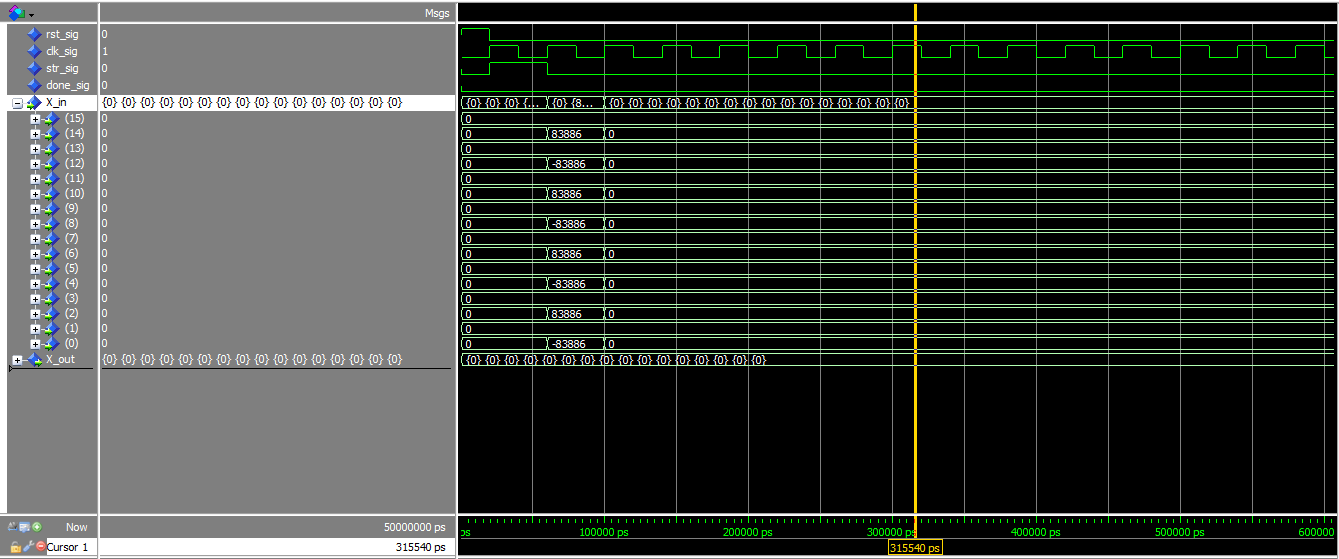
\includegraphics[scale=0.45]{test_sin/fs_sin_in.png}
    \caption{Segnale sinusoidale: dati in ingresso}
    \label{fig:sin_in}
\end{figure}\\
In Figura \ref{fig:sin_in} è osservabile l'inserimento dei dati in ingresso dopo il segnale di START.
\pagebreak
\begin{figure}[h]
    \centering
    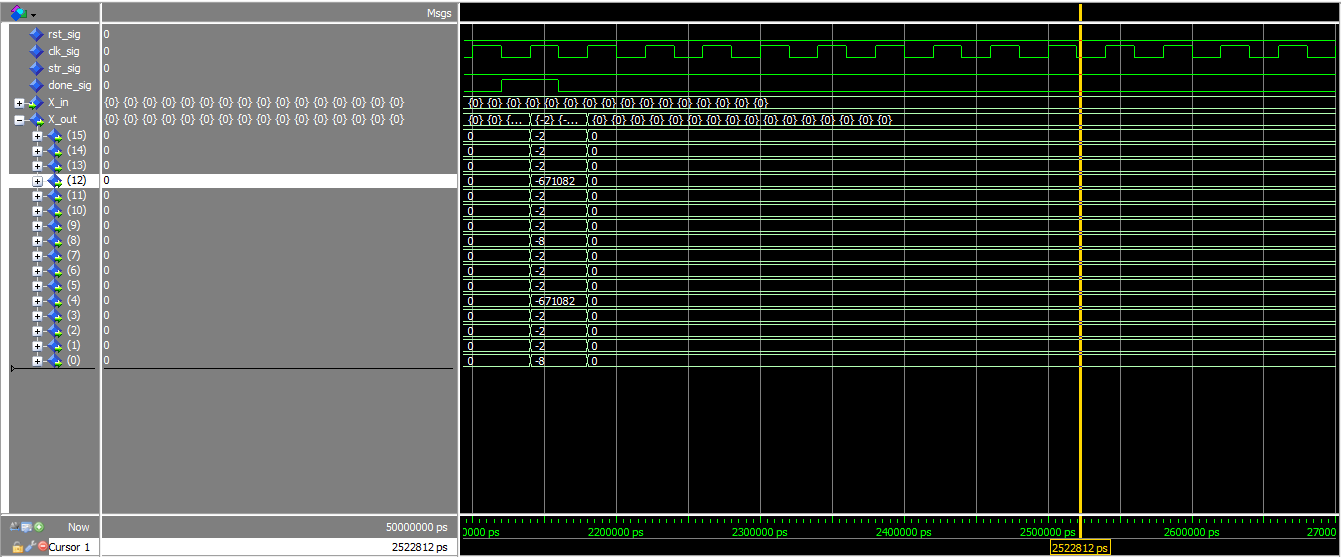
\includegraphics[scale=0.45]{test_sin/fs_sin_out.png}
    \caption{Segnale sinusoidale: dati in uscita}
    \label{fig:sin_out}
\end{figure}\\
Dalla Figura \ref{fig:sin_out} è possibile notare l'uscita della FFT. é da ricordare che l'indice 0 è nella parte inferiore della simulazione, com'è visibile dalla descrizione dei segnali nella finestra a sinistra.\\
Il valore di uscita in posizione X[4] e X[12] è X[k]=-671082 che, se riconvertito col fattore di scala e riportato nel range numerico di partenza, equivale a X[k]=$-671082*2^{-23}=-0,0799$, valore che risulta essere in linea con i risultati attesi. Inoltre anche in questo caso alcune uscite sono diverse da zero ed il motivo risiede nuovamente nelle approssimazioni e nelle conversioni dei Twiddle Factor con un formato fractional, come già spiegato in precedenza.
\begin{figure}[h]
    \centering
    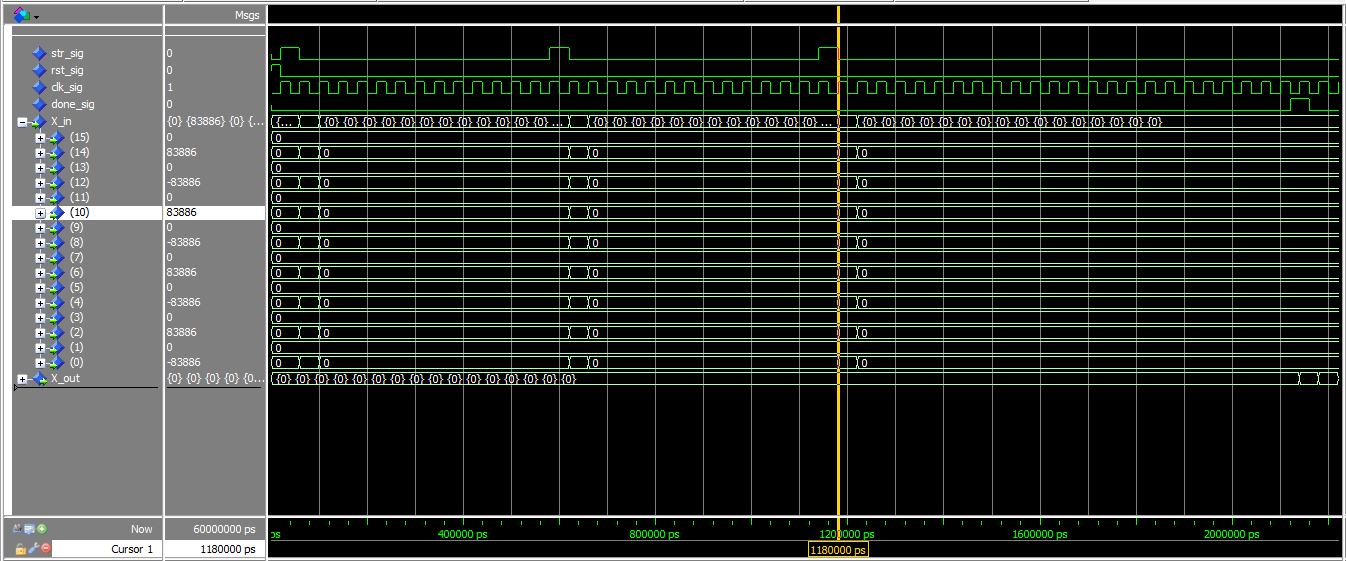
\includegraphics[scale=0.45]{test_sin/fs_sin_in_doble.png}
    \caption{Segnale sinusoidale: dati in ingresso "full speed"}
    \label{fig:sin_insin_in_doble}
\end{figure}\\
In Figura \ref{fig:sin_insin_in_doble} è presente l'inserimento dei dati in modalità full-speed.
\pagebreak
\begin{figure}[h]
    \centering
    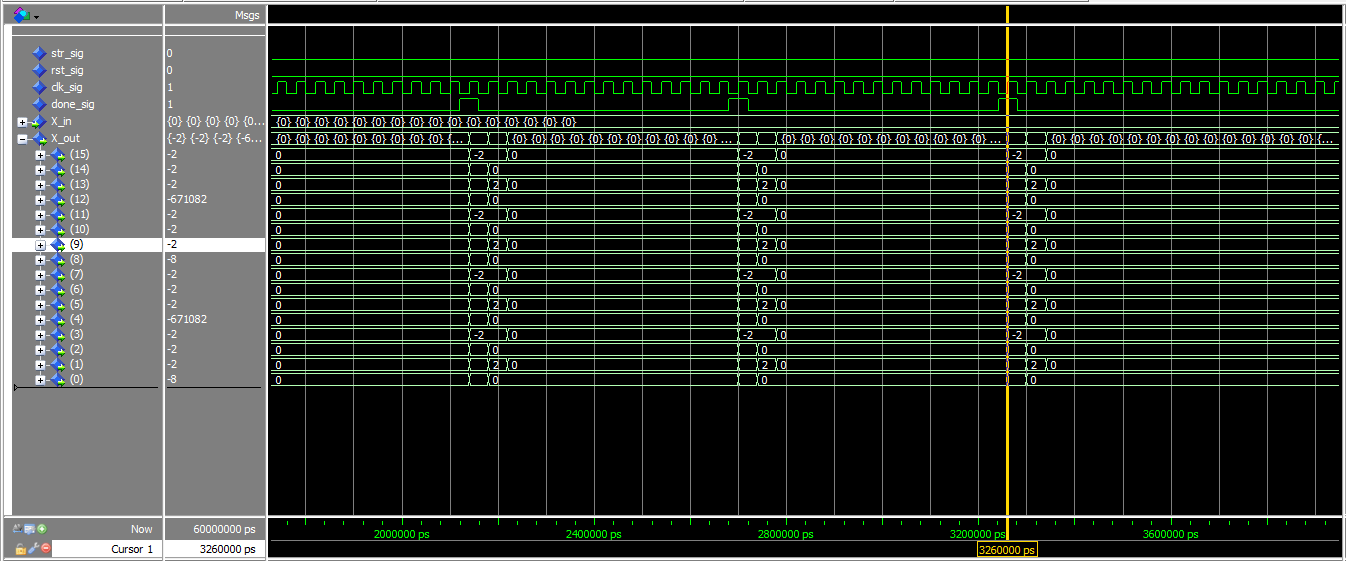
\includegraphics[scale=0.45]{test_sin/fs_sin_out_doble.png}
    \caption{Segnale sinusoidale: dati in uscita "full speed"}
    \label{fig:sin_out_doble}
\end{figure}\\
In Figura \ref{fig:sin_out_doble} è possibile osservare le uscite in modalità full-speed, di cui i valori numerici sono riportati in Tabella al sottocapitolo \ref{tab:sin}.
%%%%%%%%%%%%%%%%%%%%%%%%%%%%%%%%%%%%%%%%
\subsection{Delta di Dirac ritardata nel tempo}
In questo test è stata utilizzata una Delta di Dirac ritardata nel dominio del tempo, la cui trasformata assomiglia ad un segnale triangolare in frequenza.\\L'ampiezza della Delta è pari ad A=0,75, ma per i motivi precedentemente citati è stato scelto un valore A'=0,0075, che, riconvertito con lo scale factor, risulta essere n=62914,56, approssimato a 62915.\\Di seguito si riportato gli ingressi e le uscite di questo test:
\begin{itemize}
    \item Ingresso: x[n]=[0,0,0,0,0,0,0,0,0.75,0,0,0,0,0,0,0]
    \item Uscita:   X[k]=[0.75,-0.75,0.75,-0.75,0.75,-0.75,0.75,-0.75,0.75,-0.75,0.75,-0.75,0.75,-0.75,0.75,-0.75]
\end{itemize}
\begin{figure}[h]
    \centering
    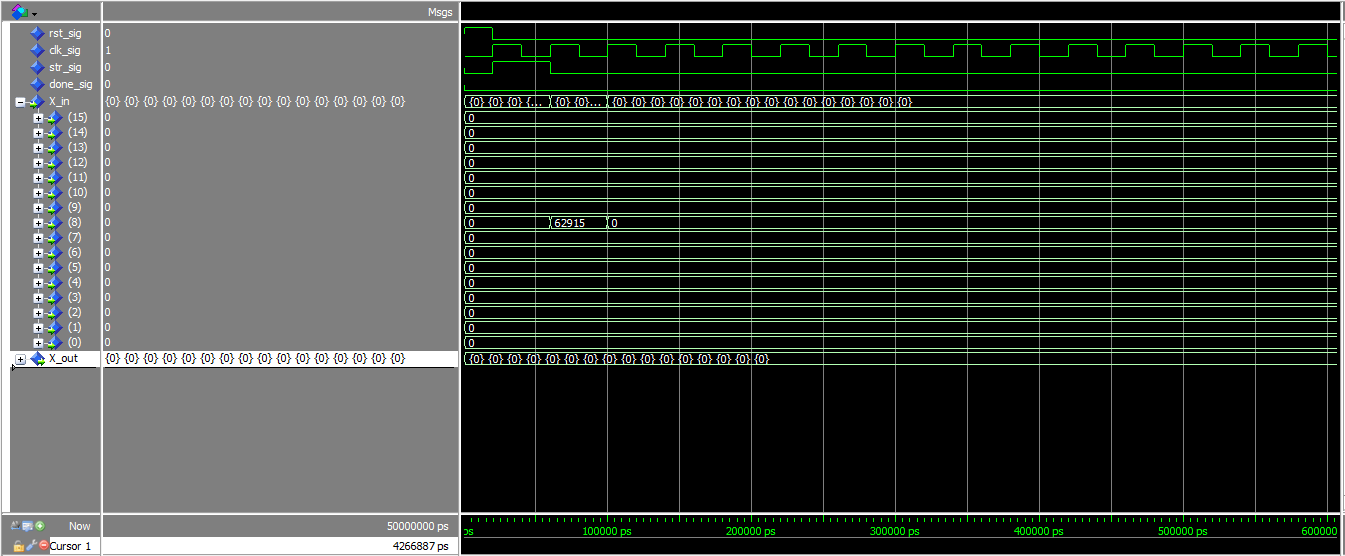
\includegraphics[scale=0.45]{test_delta_0.75/fs_d075_in.png}
    \caption{Segnale Delta di Dirac ritardata nel tempo: dati in ingresso}
    \label{fig:delta75_in}
\end{figure}
In Figura \ref{fig:delta75_in} è presente l'inserimento del vettore d'ingresso.
\pagebreak
\begin{figure}[h]
    \centering
    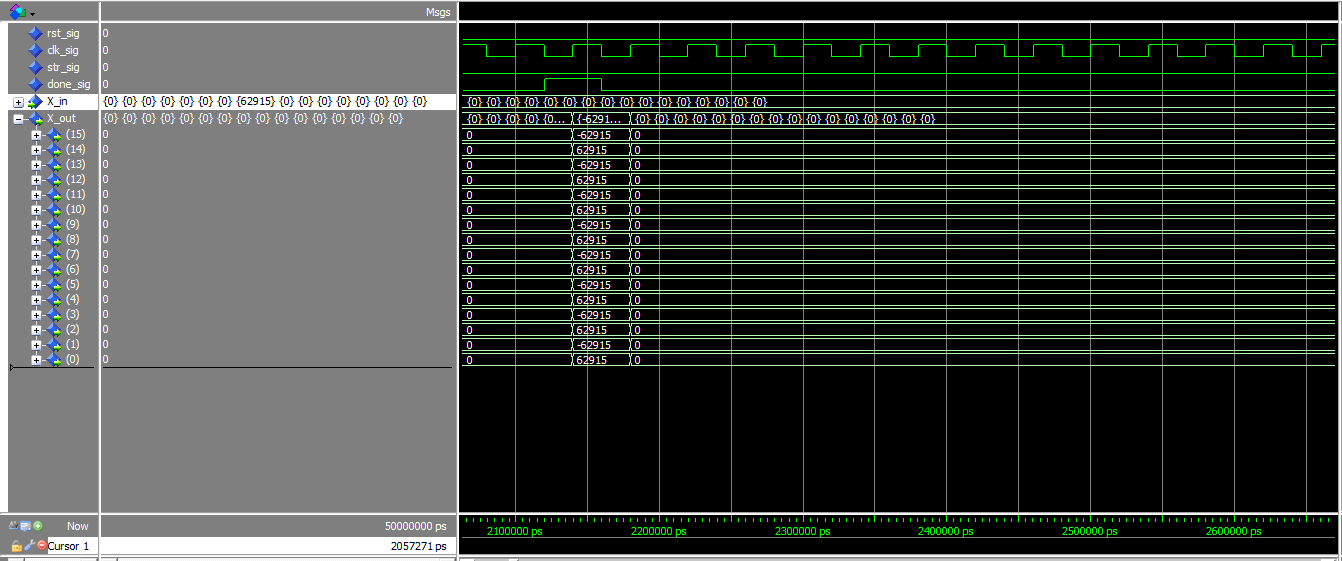
\includegraphics[scale=0.45]{test_delta_0.75/fs_d075_out.png}
    \caption{Segnale Delta di Dirac ritardata nel tempo: dati in uscita}
    \label{fig:delta75_out}
\end{figure}\\
In Figura \ref{fig:delta75_out} è riportata l'uscita dell'FFT, i cui valori di ingresso sono +62915 e -62915, che sono coerenti con le aspettative, in quanto risultano esattamente il numero posto in ingresso.
\begin{figure}[h]
    \centering
    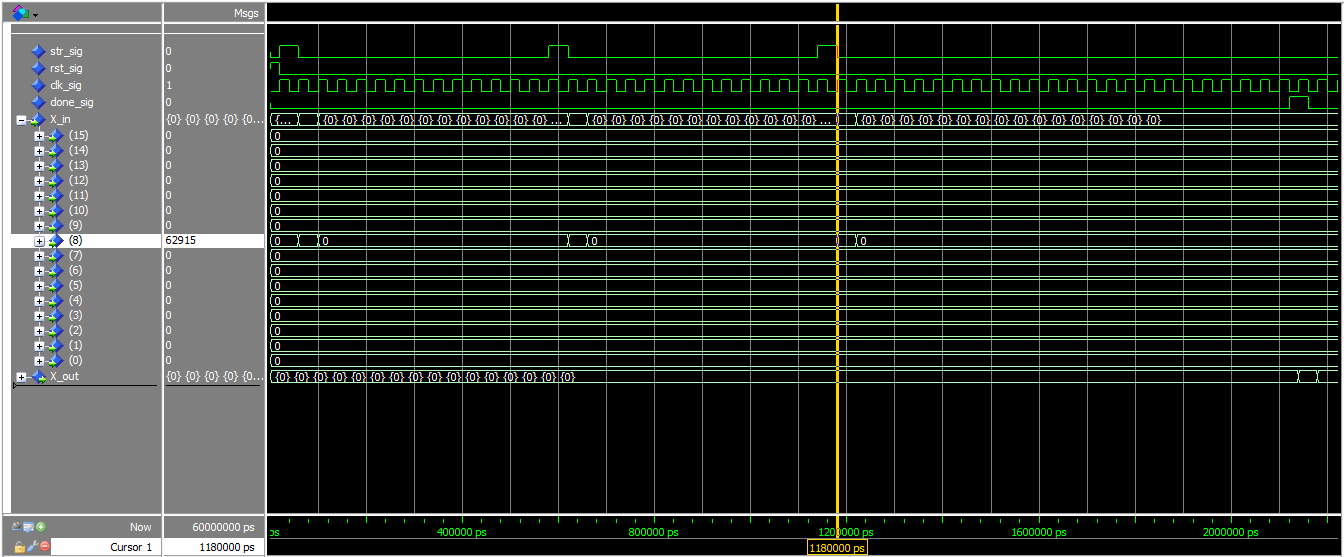
\includegraphics[scale=0.45]{test_delta_0.75/fs_d075_in_doble.png}
    \caption{Segnale Delta di Dirac ritardata nel tempo: dati in ingresso "full speed"}
    \label{fig:delta75_in_doble}
\end{figure}\\
In Figura \ref{fig:delta75_in_doble} è presente l'inserimento dei dati in modalità full speed.
\pagebreak
\begin{figure}[h]
    \centering
    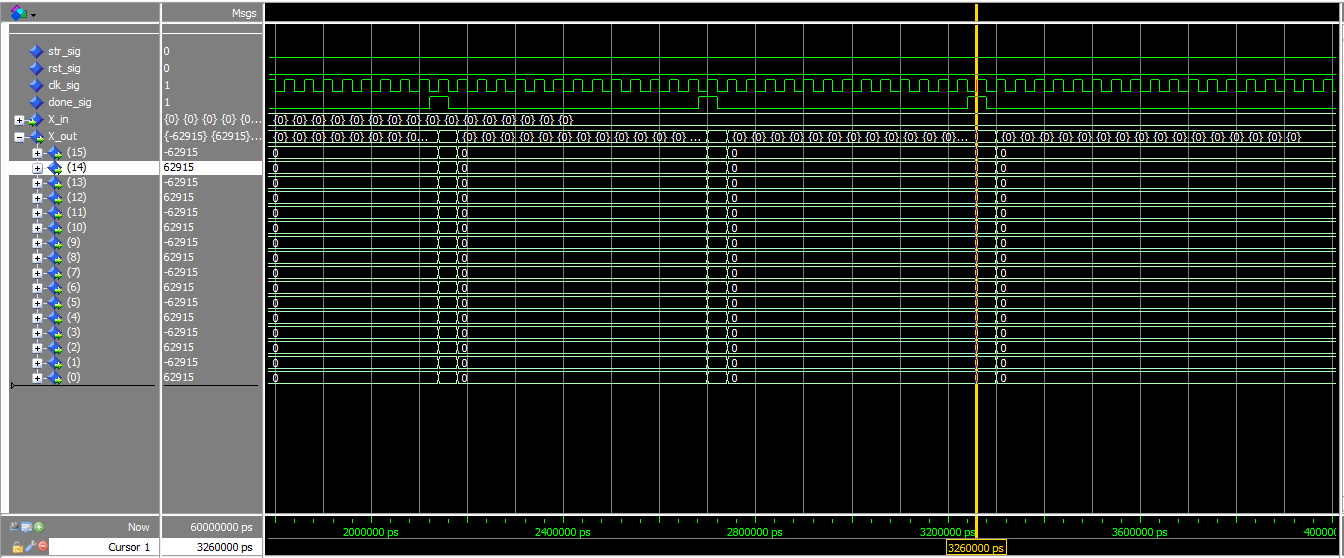
\includegraphics[scale=0.45]{test_delta_0.75/fs_d075_out_doble.png}
    \caption{Segnale Delta di Dirac ritardata nel tempo: dati in uscita "full speed"}
    \label{fig:delta75_out_doble}
\end{figure}\\
In Figura \ref{fig:delta75_out_doble} è possibile notare le tre uscite consecutive della FFT. Nella Tabella al sottocapitolo \ref{tab:delta075} si possono consultare i risultati numerici.
%%%%%%%%%%%%%%%%%%%%%%%%%%%%%%%%%%%
\subsection{Onda quadra 1}
Per questo test è stata utilizzata un'onda quadra con dinamica tra $A_+$=+1 e $A_-$=-1. I valori numerici che sono stati inseriti nel test sono i medesimi utilizzati per gli altri test, ovvero $A_+=83886$ e $A_-=-83886$.\\Di seguito sono riportati gli ingressi e le uscite:
\begin{itemize}
    \item Ingresso: x[n]=[-1,-1,+1,+1,-1,-1,+1,+1,-1,+1,-1,-1,+1,+1,-1,-1]
    \item Uscita:   X[k]=[0,0,0,0,-8+i8,0,0,0,0,0,0,0,-8-i8,0,0,0]
\end{itemize}
Particolare attenzione è da porre sulla parte "specchiata" immaginaria dello spettro. Questa, oltre ad essere ribaltata rispetto all'asse delle ordinate risulta esserlo anche rispetto all'asse delle ascisse, cambiando quindi di segno, e questo è il motivo per cui lo spettro immagine risulta essere -8-i8. Tutto ciò è dovuto alle proprietà di simmetria coniugata della Trasformata di Fourier.
\begin{figure}[h]
    \centering
    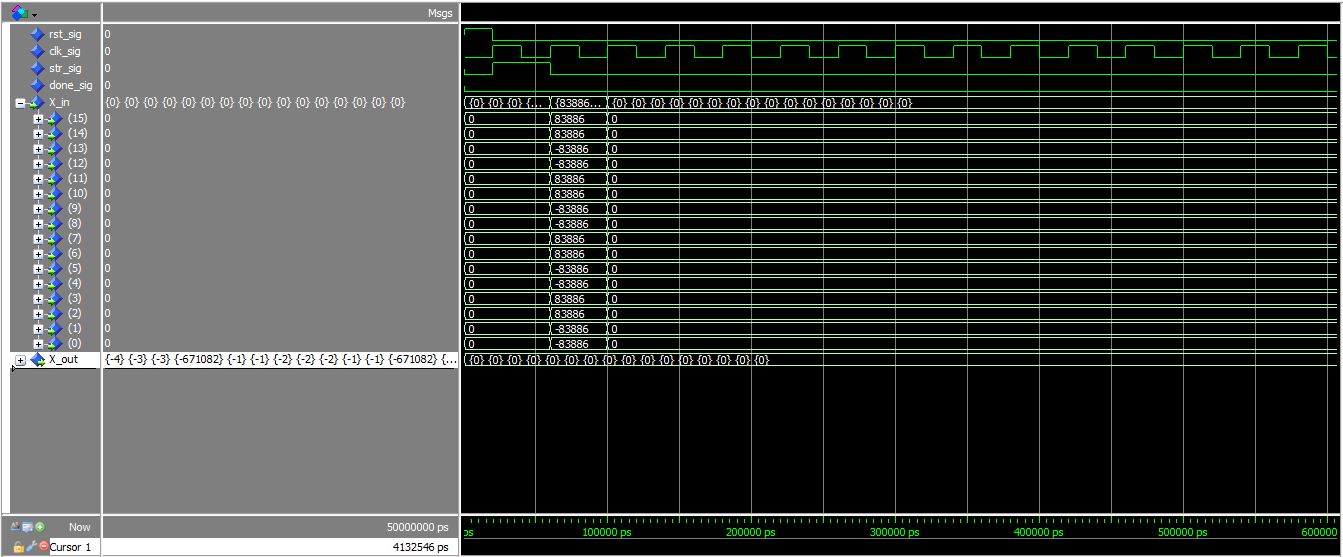
\includegraphics[scale=0.45]{test_square1/fs_square_in.png}
    \caption{Segnale Onda quadra 1: dati in ingresso}
    \label{fig:square_in}
\end{figure}\\
In Figura \ref{fig:square_in} sono osservabili i valori numerici del vettore in ingresso.
\pagebreak
\begin{figure}[h]
    \centering
    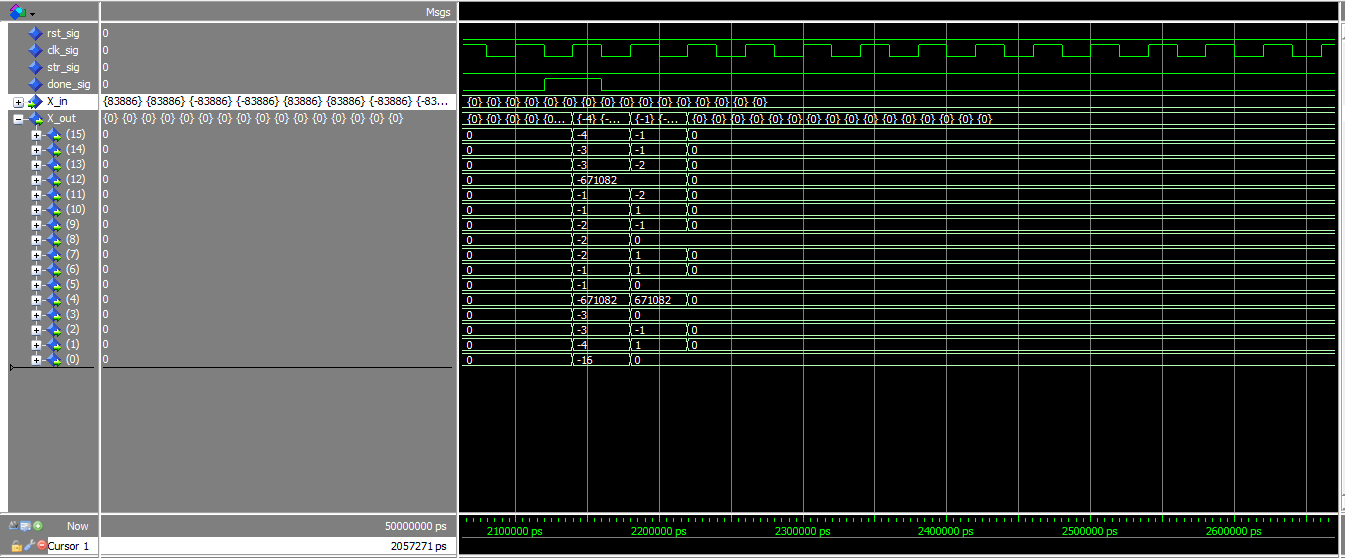
\includegraphics[scale=0.45]{test_square1/fs_square_out.png}
    \caption{Segnale Onda quadra 1: dati in uscita}
    \label{fig:square_out}
\end{figure}
\\In Figura \ref{fig:square_out} è riportata l'uscita dell'FFT, da cui partendo dal basso sono presenti l'uscita X[5]= -671082 + i671082, che, riconvertita con il fattore di scala opportuno, risulta essere X[5]=-0.0799 + i0.799, valore che confrontato all'ingresso pari a x[n]=$\pm$ 0.01 (x[n]=$\pm83886*2^{-23}$) risulta essere congruente al risultato atteso.
\begin{figure}[h]
    \centering
    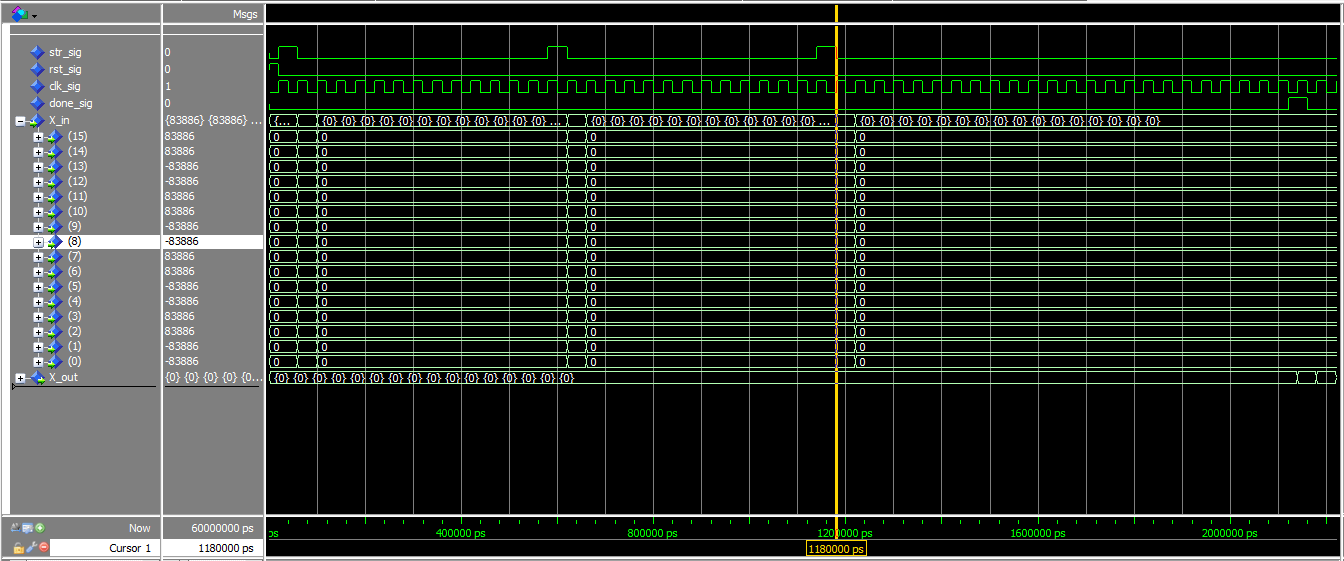
\includegraphics[scale=0.45]{test_square1/fs_square_in_doble.png}
    \caption{Segnale Onda quadra 1: dati in ingresso "full speed"}
    \label{fig:square_in_doble}
\end{figure}\\
In Figura \ref{fig:square_in_doble} è reperibile l'inserimento dei dati in modalità full speed.
\pagebreak
\begin{figure}[h]
    \centering
    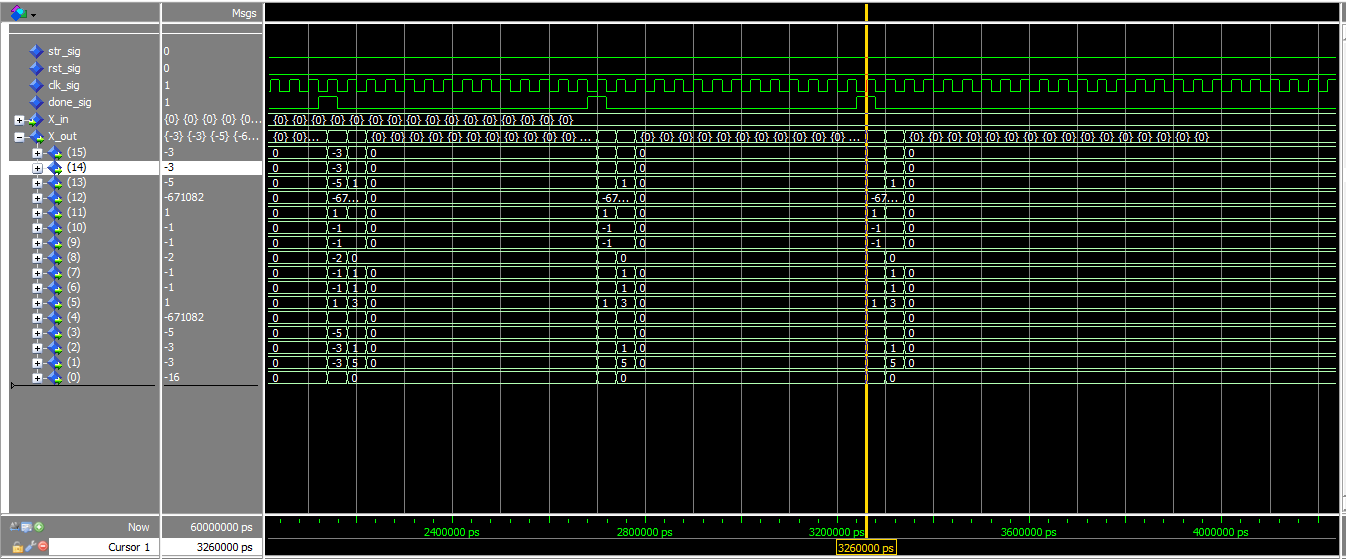
\includegraphics[scale=0.45]{test_square1/fs_square_out_doble.png}
    \caption{Segnale Onda quadra 1: dati in uscita "full speed"}
    \label{fig:square_out_doble}
\end{figure}\\
Le tre uscite consecutive della FFT invece sono visibili in Figura \ref{fig:square_out_doble}.
\begin{figure}[h]
    \centering
    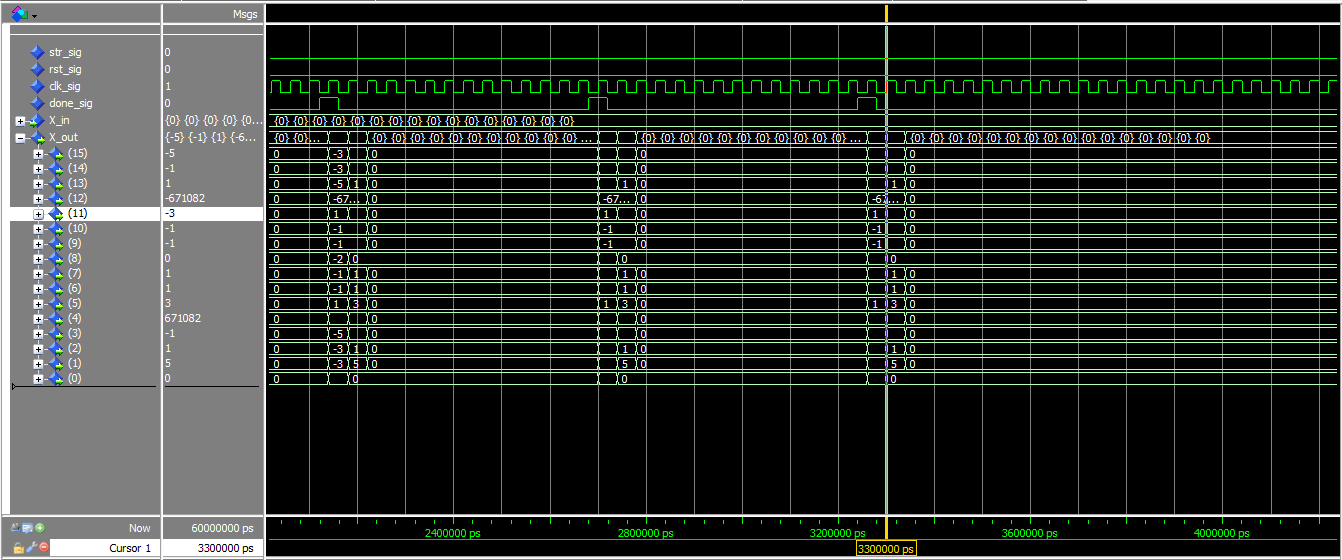
\includegraphics[scale=0.45]{test_square1/zoom_2nd_out.png}
    \caption{Segnale Onda quadra 1: zoom dati in uscita "full speed"}
    \label{fig:square_out_zoom}
\end{figure}\\
In Figura \ref{fig:square_out_zoom} è stato fatto uno zoom sulla terza uscita consecutiva così da mostrare i dati.\\
Nella Tabella al sottocapitolo \ref{tab:quadra1} si possono consultare i risultati numerici.
%%%%%%%%%%%%%%%%%%%%%%%%%%%%%
\pagebreak
\subsection{Onda quadra 2}
Per questo test è stata utilizzata un'onda quadra con dinamica tra $A_+$=+0,5 e $A_-$=-0,5 con periodo diverso rispetto al segnale precedente. Qui i valori numerici inseriti nel test sono $A'_+$=+41943   $A'_-$=-41943, corrispondenti quindi ad una dinamica pari a D=$\pm$0,005, che rispetta quindi i vincoli sull'ingresso.\\Di seguito sono riportati gli ingressi e le uscite di tale test:
\begin{itemize}
    \item Ingresso: x[n]=[0.5,0.5,0.5,0.5,0.5,0.5,0.5,0.5,0.5,-0.5,-0.5,-0.5,-0.5,-0.5,-0.5,-0.5]
    \item Uscita:   X[k]=[1,-i5.027,1,-i1.497,1,-i0.668,1,-i0.199,1,+i0.199,1,+i0.668,1,+i1.497,1,+i5.027]
\end{itemize}
Anche in questo caso la parte immaginaria dello spettro immagine risulta non solo specchiata, ma anche cambiata di segno.
\begin{figure}[h]
    \centering
    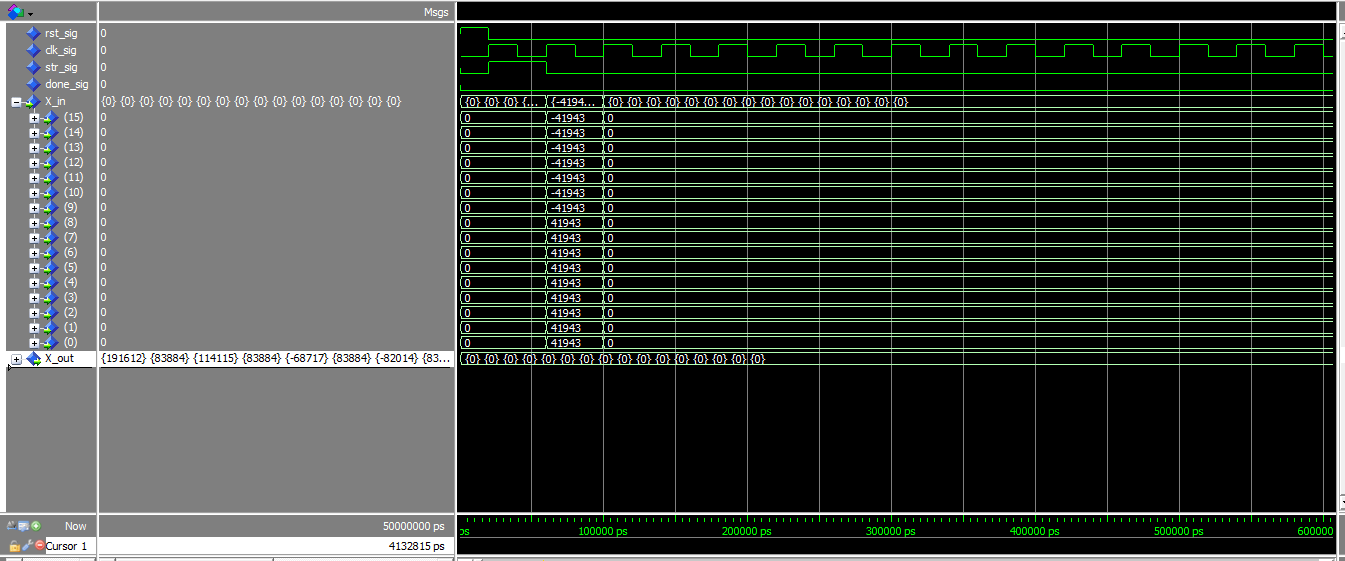
\includegraphics[scale=0.45]{test_square2/fs_q(+5 -5)_in.png}
    \caption{Segnale Onda quadra 2: dati in ingresso}
    \label{fig:square2_in}
\end{figure}
\\In Figura \ref{fig:square_in} è presente l'inserimento del vettore di ingresso.
\begin{figure}[h]
    \centering
    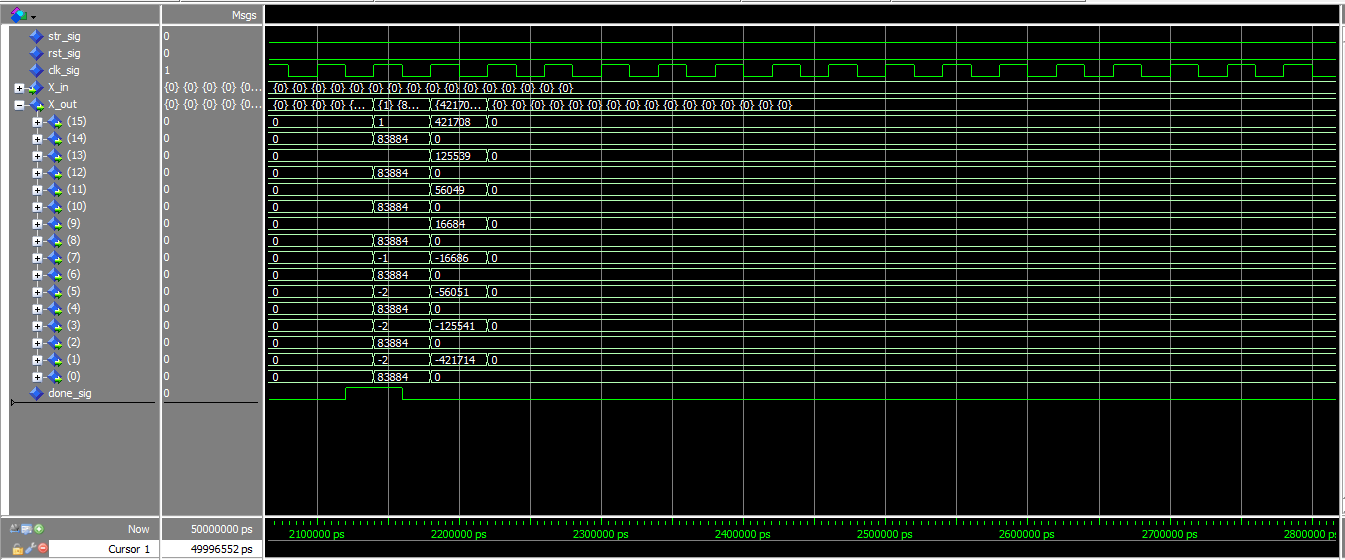
\includegraphics[scale=0.45]{test_square2/fs_q(+5-5)_out.png}
    \caption{Segnale Onda quadra 2: dati in uscita}
    \label{fig:square2_out}
\end{figure}\\
In Figura \ref{fig:square2_out} invece è possibile osservare l'uscita dell'FFT, in cui nuovamente alcuni output, che dovrebbero essere zero, non lo sono a causa dei motivi elencati in precedenza.\\ Inoltre sulla parte immagine dello specchio sono presenti delle piccole differenze sulle uscite. Questo fenomeno è nuovamente generato dalle approssimazioni introdotte dal sistema. Le uscite sono coerenti a quanto atteso, per i valori numerici si faccia riferimento alla Tabella al sottocapitolo \ref{tab:quadra2}.
\pagebreak
\begin{figure}[h]
    \centering
    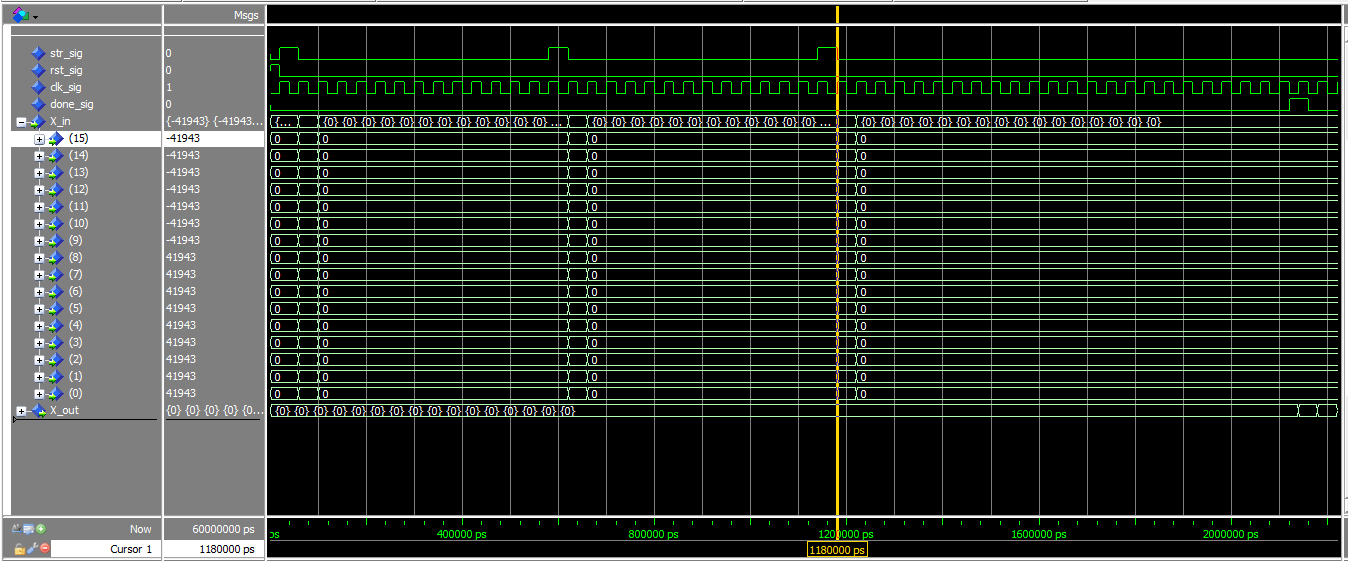
\includegraphics[scale=0.45]{test_square2/fs_q(+5 -5)_in_doble.png}
    \caption{Segnale Onda quadra 2: dati in ingresso "full speed"}
    \label{fig:square2_in_doble}
\end{figure}
\\In Figura \ref{fig:square_in_doble} è disponibile l'inserimento dei dati in modalità full speed.
\begin{figure}[h]
    \centering
    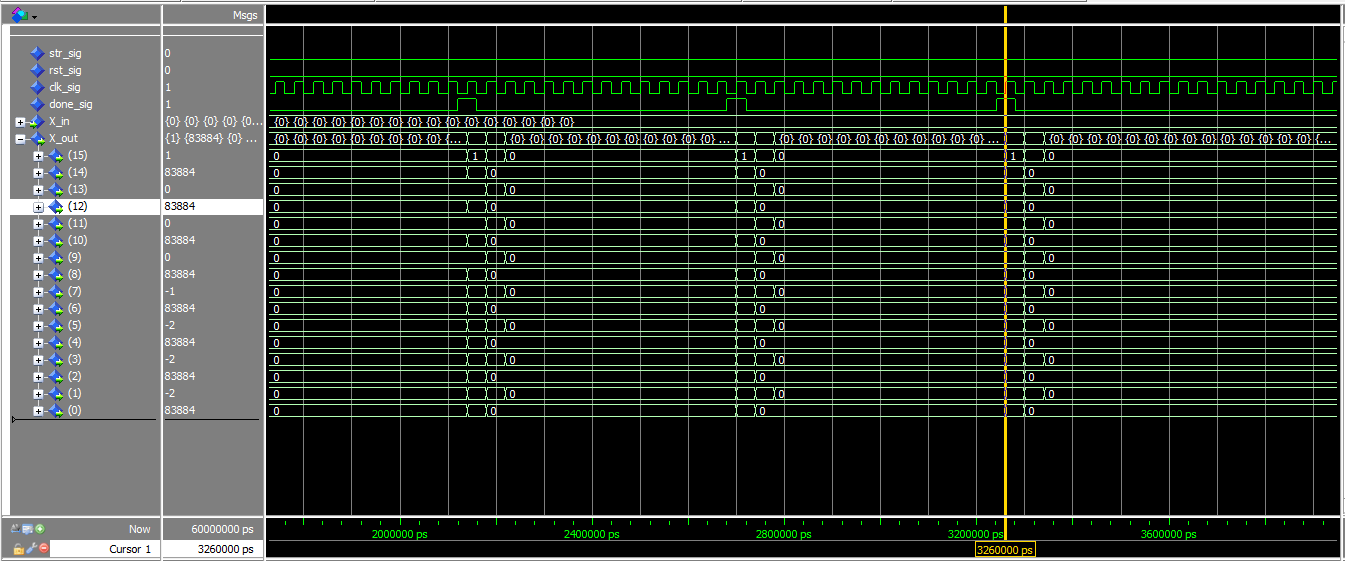
\includegraphics[scale=0.45]{test_square2/fs_q(+5-5)_out_doble1.png}
    \caption{Segnale Onda quadra 2: dati in uscita "full speed"}
    \label{fig:square2_out_doble1}
\end{figure}
\\In Figura \ref{fig:square2_out_doble1} è visibile l'uscita reale della FFT in modalità full speed.
\pagebreak
\begin{figure}[h]
    \centering
    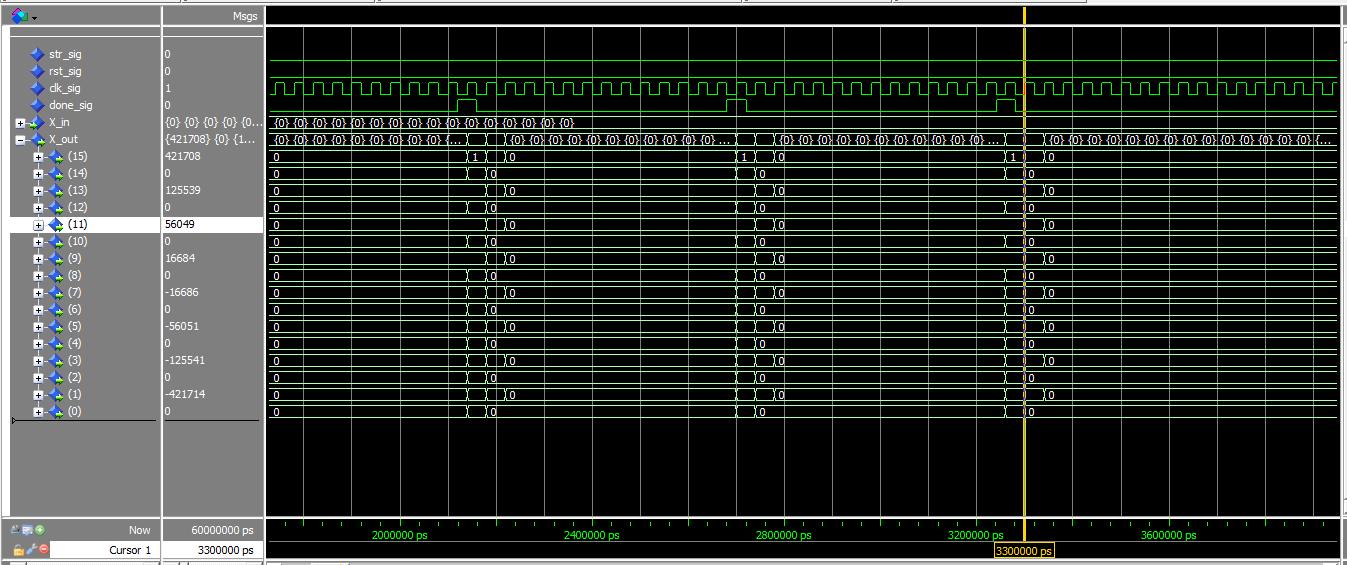
\includegraphics[scale=0.45]{test_square2/fs_q(+5-5)_out_doble2.png}
    \caption{Segnale Onda quadra 2:  dati in uscita "full speed"}
    \label{fig:square2_out_doble2}
\end{figure}
\\In Figura \ref{fig:square2_out_doble2} è riportata l'uscita immaginaria della FFT in modalità full speed.
Nella Tabella al sottocapitolo \ref{tab:quadra2} si possono consultare i risultati numerici.
%%%%%%%%%%%%%%%%%%%%%%%%%%%%%%
\newpage
\section{Tabelle}
\subsection{Twiddle Factor}
\begin{longtable}{*3c}
\caption{Twiddle Factor parte Reale}
\label{Twiddle Factor reale}\\
\toprule
W\ped{R} & Valore numerico &  C2 W\ped{R} su 24 bit \\
\midrule
\endfirsthead
W\ped{R} & Valore numerico &  C2 W\ped{R} su 24 bit \\
\midrule
\endhead
\midrule
\endfoot
\bottomrule
\endlastfoot
W0 & 0,9999998808 &	011111111111111111111111\\
W1 & 0,92387953251129 & 011101100100000110101111\\
W2 & 0,70710678118655 & 010110101000001001111001\\
W3 & 0,38268343236509 & 001100001111101111000101\\
W4 & 0 & 000000000000000000000000\\
W5 & -0,38268343236509 & 110011110000010000111011\\
W6 & -0,70710678118655 & 101001010111110110000111\\
W7 & -0,92387953251129 & 100010011011111001010001\\
\end{longtable}
\begin{longtable}{*3c}
\caption{Twiddle Factor parte Immaginaria}
\label{Twiddle Factor immaginaria}\\
\toprule
 W\ped{I} & Valore numerico &  C2 W\ped{I} su 24 bit \\
\midrule
\endfirsthead
 W\ped{I} & Valore numerico &  C2 W\ped{I} su 24 bit \\
\midrule
\endhead
\midrule
\endfoot
\bottomrule
\endlastfoot
W0	& 0	& 000000000000000000000000\\
W1	& -0,38268343236509 & 110011110000010000111011\\
W2	& -0,70710678118655 & 101001010111110110000111\\
W3	& -0,92387953251129 & 100010011011111001010001\\
W4	& -1 & 100000000000000000000000\\
W5	& -0,92387953251129 & 100010011011111001010001\\
W6	& -0,70710678118655 & 101001010111110110000111\\
W7	& -0,38268343236509 & 110011110000010000111011\\
\end{longtable}
%%%%%%%%%%%%%%%%%%%%%%  1  %%%%%%%%%%%%%%%%%%%%%%%%% 
\subsection{Delta di Dirac } \label{tab:delta}
\begin{longtable}{*5c}
\caption{Dati reali(K=23)}
\label{}\\
\toprule
n & Xin Re & Xin Im & Xout Re & Xout Im \\
\midrule
\endfirsthead
n & Xin Re & Xin Im & Xout Re & Xout Im \\
\midrule
\endhead
\midrule
\endfoot
\bottomrule
\endlastfoot
0 & 0,01 & 0 & 0,01 & 0\\
1 & 0    & 0 & 0,01 & 0 \\
2 & 0    & 0 & 0,01 & 0 \\
3 & 0    & 0 & 0,01 & 0 \\
4 & 0    & 0 & 0,01 & 0 \\
5 & 0    & 0 & 0,01 & 0 \\
6 & 0    & 0 & 0,01 & 0 \\
7 & 0    & 0 & 0,01 & 0 \\
8 & 0    & 0 & 0,01 & 0 \\
9 & 0    & 0 & 0,01 & 0 \\
10& 0    & 0 & 0,01 & 0 \\
11& 0    & 0 & 0,01 & 0 \\
12& 0    & 0 & 0,01 & 0 \\
13& 0    & 0 & 0,01 & 0 \\
14& 0    & 0 & 0,01 & 0 \\
15 & 0 & 0 & 0,01 & 0 \\ 
\end{longtable}
\begin{longtable}{*5c}
\caption{Dati non scalati}
\label{}\\
\toprule
n & Xin Re & Xin Im & Xout Re & Xout Im \\
\midrule
\endfirsthead
n & Xin Re & Xin Im & Xout Re & Xout Im \\
\midrule
\endhead
\midrule
\endfoot
\bottomrule
\endlastfoot
0 & 83886 & 0 & 83886 & 0\\
1 & 0    & 0 & 83886 & 0 \\
2 & 0    & 0 & 83886 & 0 \\
3 & 0    & 0 & 83886 & 0 \\
4 & 0    & 0 & 83886 & 0 \\
5 & 0    & 0 & 83886 & 0 \\
6 & 0    & 0 & 83886 & 0 \\
7 & 0    & 0 & 83886 & 0 \\
8 & 0    & 0 & 83886 & 0 \\
9 & 0    & 0 & 83886 & 0 \\
10& 0    & 0 & 83886 & 0 \\
11& 0    & 0 & 83886 & 0 \\
12& 0    & 0 & 83886 & 0 \\
13& 0    & 0 & 83886 & 0 \\
14& 0    & 0 & 83886 & 0 \\
15 & 0 & 0 & 83886 & 0 \\ 
\end{longtable}
\begin{longtable}{*3c}
\caption{Test}
\label{}\\
\toprule
n & Xin & Xout\\
\midrule
\endfirsthead
n & Xin & Xout\\
\midrule
\endhead
\midrule
\endfoot
\bottomrule
\endlastfoot
0 & 1& 1\\
1 & 0& 1\\
2 & 0& 1\\
3 & 0& 1\\
4 & 0& 1\\
5 & 0& 1\\
6 & 0& 1\\
7 & 0& 1 \\
8 & 0& 1 \\
9 & 0& 1\\
10& 0& 1\\
11& 0& 1\\
12& 0& 1\\
13& 0& 1\\
14& 0& 1\\
15 &0& 1\\ 
\end{longtable}
%%%%%%%%%%%%%%%%%%%%  2 %%%%%%%%%%%%%%%%%%%%%%%%%%
\newpage
\subsection{Costante -1} \label{tab:const}
\begin{longtable}{*5c}
\caption{Dati reali(K=23)}
\label{}\\
\toprule
n & Xin Re & Xin Im & Xout Re & Xout Im \\
\midrule
\endfirsthead
n & Xin Re & Xin Im & Xout Re & Xout Im \\
\midrule
\endhead
\midrule
\endfoot
\bottomrule
\endlastfoot
0 & -0,01 & -0,160 & 0,01 & 0\\
1 & -0,01 & 0 & -2,3841910$^{-7}$ & 0\\
2 & -0,01 & 0 & -3,5762810$^{-7}$ &-1,19209 10$^{-7}$\\
3 & -0,01 & 0 & -1,1920910$^{-7}$ & 1,19209 10$^{-7}$\\
4 & -0,01& 0 & -2,3841910$^{-7}$ & 2,38419 10$^{-7}$\\
5 & -0,01& 0 & -2,3841910$^{-7}$ & 3,57628 10$^{-7}$\\
6 & -0,01 & 0 & -1,1920910$^{-7}$ & 1,19209 10$^{-7}$\\
7 & -0,01 & 0 & -2,3841910$^{-7}$& 1,19209 10$^{-7}$\\
8 & -0,01& 0 &-2,3841910$^{-7}$ & 0,00000\\
9 & -0,01& 0 & -2,3841910$^{-7}$ & -2,38419 10$^{-7}$\\
10& -0,01& 0 & -1,1920910$^{-7}$ & 1,19209 10$^{-7}$\\
11& -0,01& 0 & -1,1920910$^{-7}$ & -1,19209 10$^{-7}$\\
12& -0,01 & 0 &-2,3841910$^{-7}$ & -2,38419 10$^{-7}$\\
13& -0,01& 0 & -7,1525610$^{-7}$ & -3,57628 10$^{-7}$\\
14& -0,01& 0 &-3,5762810$^{-7}$ & -1,19209 10$^{-7}$\\
15 & -0,01& 0 & -7,1525610$^{-7}$ & -1,19209 10$^{-7}$\\ 
\end{longtable}
\begin{longtable}{*5c}
\caption{Dati non scalati}
\label{}\\
\toprule
n & Xin Re & Xin Im & Xout Re & Xout Im \\
\midrule
\endfirsthead
n & Xin Re & Xin Im & Xout Re & Xout Im \\
\midrule
\endhead
\midrule
\endfoot
\bottomrule
\endlastfoot
0 & -83886 & 0 & -1,34218 10$^{-6}$ & 0\\
1 & -83886    & 0 & -2 & 0 \\
2 & -83886    & 0 & -3 & -1 \\
3 & -83886    & 0 & -1 & 1 \\
4 & -83886    & 0 & -2 & 2 \\
5 & -83886    & 0 & -2 & 3 \\
6 & -83886    & 0 & -1 & 1 \\
7 & -83886    & 0 & -2 & 1 \\
8 & -83886    & 0 & -2 & 0 \\
9 & -83886    & 0 & -2 & -2 \\
10& -83886    & 0 & -1 & 1 \\
11& -83886    & 0 & -1 & -1 \\
12& -83886    & 0 & -2 & -2 \\
13& -83886    & 0 & -6 & -3 \\
14& -83886    & 0 & -3 & -1 \\
15 & -83886 & 0 & -6 & -1 \\ 
\end{longtable}
\newpage
\begin{longtable}{*3c}
\caption{Test}
\label{}\\
\toprule
n & Xin & Xout\\
\midrule
\endfirsthead
n & Xin & Xout\\
\midrule
\endhead
\midrule
\endfoot
\bottomrule
\endlastfoot
0 & -1& -16\\
1 & -1& 0\\
2 & -1& 0\\
3 & -1& 0\\
4 & -1& 0\\
5 & -1& 0\\
6 & -1& 0\\
7 & -1& 0 \\
8 & -1& 0 \\
9 & -1& 0\\
10& -1& 0\\
11& -1& 0\\
12& -1& 0\\
13& -1& 0\\
14& 0& 0\\
15& 0& 0\\ 
\end{longtable}
%%%%%%%%%%%%%%%%%%%% 3  %%%%%%%%%%%%%%%%%%%%%%%%%%%%%
\subsection{Sinusoide}\label{tab:sin}
\begin{longtable}{*5c}
\caption{Dati reali(K=23)}
\label{}\\
\toprule
n & Xin Re & Xin Im & Xout Re & Xout Im \\
\midrule
\endfirsthead
n & Xin Re & Xin Im & Xout Re & Xout Im \\
\midrule
\endhead
\midrule
\endfoot
\bottomrule
\endlastfoot
0 & -0,01 & 0 & -9,5 10$^{-7}$ & 0\\
1 & 0,00   & 0 & -2,4 10$^{-7}$ & 0\\
2 & 0,01    & 0 & -2,4 10$^{-7}$ & 0\\
3 & 0,00   & 0 & -2,4 10$^{-7}$ & 0 \\
4 & -0,01    & 0 & -0,08 & 0\\
5 & 0,00    & 0 & -2,4 10$^{-7}$ & 0\\
6 & 0,01    & 0 & -2,4 10$^{-7}$& 0\\
7 & 0,00    & 0 & -2,4 10$^{-7}$ & 0\\
8 & -0,01    & 0 & -9,5 10$^{-7}$ & 0\\
9 & 0,00    & 0 & -2,4 10$^{-7}$ & 0\\
10& 0,01    & 0 & -2,4 10$^{-7}$ & 0 \\
11& 0,00    & 0 & -2,4 10$^{-7}$ & 0\\
12& -0,01    & 0 & -0,08 & 0\\
13& 0,00    & 0 & -2,4 10$^{-7}$ & 0\\
14& 0,01    & 0 & -2,4 10$^{-7}$& 0\\
15 & 0,00 & 0 & -2,4 10$^{-7}$ & 0\\ 
\end{longtable}
\newpage
\begin{longtable}{*5c}
\caption{Dati non scalati}
\label{}\\
\toprule
n & Xin Re & Xin Im & Xout Re & Xout Im \\
\midrule
\endfirsthead
n & Xin Re & Xin Im & Xout Re & Xout Im \\
\midrule
\endhead
\midrule
\endfoot
\bottomrule
\endlastfoot
0 & -83886 & 0 & -8 & 0\\
1 & 0    & 0 & -2 & 0 \\
2 & 83886    & 0 & -2 & 0 \\
3 & 0    & 0 & -2 & 0 \\
4 & -83886    & 0 & -671082 & 0 \\
5 & 0    & 0 & -2 & 0 \\
6 & 83886    & 0 & -2 & 0 \\
7 & 0    & 0 & -2 & 0 \\
8 & -83886    & 0 & -8 & 0 \\
9 & 0    & 0 & -2 & 0 \\
10& 83886    & 0 & -2 & 0 \\
11& 0    & 0 & -2 & 0 \\
12& -83886    & 0 & -671082 & 0 \\
13& 0    & 0 & -2 & 0 \\
14& 83886    & 0 & -2 & 0 \\
15 & 0 & 0 & -2 & 0 \\ 
\end{longtable}
\begin{longtable}{*3c}
\caption{Test}
\label{}\\
\toprule
n & Xin & Xout\\
\midrule
\endfirsthead
n & Xin & Xout\\
\midrule
\endhead
\midrule
\endfoot
\bottomrule
\endlastfoot
0 & -1& 0\\
1 & 0& 0\\
2 & 1& 0\\
3 & 0& 0\\
4 & -1& -8\\
5 & 0& 0\\
6 & 1& 0\\
7 & 0& 0 \\
8 & -1& 0 \\
9 & 0& 0\\
10& 1& 0\\
11& 0& 0\\
12& -1& -8\\
13& 0& 0\\
14& 1& 0\\
15& 0& 0\\ 
\end{longtable}
%%%%%%%%%%%%%%%%%%%%% 4  %%%%%%%%%%%%%%%%%%%%%%%%%%%%%
\newpage
\subsection{Delta 0.75} \label{tab:delta075}
\begin{longtable}{*5c}
\caption{Dati reali(K=23)}
\label{}\\
\toprule
n & Xin Re & Xin Im & Xout Re & Xout Im \\
\midrule
\endfirsthead
n & Xin Re & Xin Im & Xout Re & Xout Im \\
\midrule
\endhead
\midrule
\endfoot
\bottomrule
\endlastfoot
0 & 0 & 0 & 0,01 & 0,0075\\
1 & 0   & 0 & 0,01 & -0,0075 \\
2 & 0    & 0 & 0,01 & 0,0075 \\
3 & 0    & 0 & 0,01 & -0,0075 \\
4 & 0    & 0 & 0,01 & 0,0075 \\
5 & 0    & 0 & 0,01 & -0,0075 \\
6 & 0    & 0 & 0,01 & 0,0075 \\
7 & 0    & 0 & 0,01 & -0,0075 \\
8 & 0,01    & 0 & 0,01 & 0,0075 \\
9 & 0    & 0 & 0,01 & -0,0075 \\
10& 0    & 0 & 0,01 & 0,0075 \\
11& 0    & 0 & 0,01 & -0,0075 \\
12& 0    & 0 & 0,01 & 0,0075 \\
13& 0    & 0 & 0,01 & -0,0075 \\
14& 0    & 0 & 0,01 & 0,0075 \\
15 & 0 & 0 & 0,01 & -0,0075 \\ 
\end{longtable}
\begin{longtable}{*5c}
\caption{Dati non scalati}
\label{}\\
\toprule
n & Xin Re & Xin Im & Xout Re & Xout Im \\
\midrule
\endfirsthead
n & Xin Re & Xin Im & Xout Re & Xout Im \\
\midrule
\endhead
\midrule
\endfoot
\bottomrule
\endlastfoot
0 & 0 & 0 & 83886 & 62915\\
1 & 0    & 0 & 83886 & -62915 \\
2 & 0    & 0 & 83886 & 62915 \\
3 & 0    & 0 & 83886 & -62915 \\
4 & 0    & 0 & 83886 & 62915 \\
5 & 0    & 0 & 83886 & -62915 \\
6 & 0    & 0 & 83886 & 62915 \\
7 & 0    & 0 & 83886 & -62915 \\
8 & 62915    & 0 & 83886 & 62915 \\
9 & 0    & 0 & 83886 & -62915 \\
10& 0    & 0 & 83886 & 62915 \\
11& 0    & 0 & 83886 & -62915 \\
12& 0    & 0 & 83886 & 62915 \\
13& 0    & 0 & 83886 & -62915 \\
14& 0    & 0 & 83886 & 62915 \\
15 & 0 & 0 & 83886 & -62915 \\ 
\end{longtable}
\newpage
\begin{longtable}{*3c}
\caption{Test}
\label{}\\
\toprule
n & Xin & Xout\\
\midrule
\endfirsthead
n & Xin & Xout\\
\midrule
\endhead
\midrule
\endfoot
\bottomrule
\endlastfoot
0 & 0& 0,75\\
1 & 0& -0,75\\
2 & 0& 0,75\\
3 & 0& -0,75\\
4 & 0& 0,75\\
5 & 0& -0,75\\
6 & 0& 0,75\\
7 & 0& -0,75 \\
8 & 0,75& 0,75 \\
9 & 0& -0,75\\
10& 0& 0,75\\
11& 0& -0,75\\
12& 0& 0,75\\
13& 0& -0,75\\
14& 0& 0,75\\
15& 0& -0,75\\ 
\end{longtable}
%%%%%%%%%%%%%%%%%%%% 5  %%%%%%%%%%%%%%%%%%%%%%%%%%
\subsection{Onda quadra 1}\label{tab:quadra1}
\begin{longtable}{*5c}
\caption{Dati reali(K=23)}
\label{}\\
\toprule
n & Xin Re & Xin Im & Xout Re & Xout Im \\
\midrule
\endfirsthead
n & Xin Re & Xin Im & Xout Re & Xout Im \\
\midrule
\endhead
\midrule
\endfoot
\bottomrule
\endlastfoot
0 & -0,01 & 0 & 0 & -1,2 10$^{-7}$\\
1 & -0,01   & 0 & 0 & -1,2 10$^{-7}$\\
2 & 0,01    & 0 & 0 & -2,4 10$^{-7}$\\
3 & 0,01   & 0 & -0,08 & -0,08 \\
4 & -0,01    & 0 & 0 & -2,4 10$^{-7}$\\
5 & -0,01    & 0 & 0 & 1,19 10$^{-7}$\\
6 & 0,01    & 0 & 0 & -1,2 10$^{-7}$\\
7 & 0,01    & 0 & 0 & 0\\
8 & -0,01    & 0 & 0 & 1,19 10$^{-7}$\\
9 & -0,01    & 0 & 0 & 1,19 10$^{-7}$\\
10& 0,01    & 0 & 0 & 0 \\
11& 0,01    & 0 & -0,08 & 0,079999\\
12& -0,01    & 0 & 0 & -1,2 10$^{-7}$\\
13& -0,01    & 0 & 0 & 1,19 10$^{-7}$\\
14& 0,01    & 0 & 0 & 0\\
15 & 0,01 & 0 & 0 & -0,0075 \\ 
\end{longtable}
\newpage
\begin{longtable}{*5c}
\caption{Dati non scalati}
\label{}\\
\toprule
n & Xin Re & Xin Im & Xout Re & Xout Im \\
\midrule
\endfirsthead
n & Xin Re & Xin Im & Xout Re & Xout Im \\
\midrule
\endhead
\midrule
\endfoot
\bottomrule
\endlastfoot
0 & -83886 & 0 & -4 & -1\\
1 & -83886    & 0 & -2 & -1 \\
2 & 83886    & 0 & -3 & -2 \\
3 & 83886    & 0 & -671082 & -671082 \\
4 & -83886    & 0 & -2 & -2 \\
5 & -83886    & 0 & -2 & 1 \\
6 & 83886    & 0 & -1 & -1 \\
7 & 83886    & 0 & -2 & 0 \\
8 & -83886    & 0 & -2 & 1 \\
9 & -83886    & 0 & -2 & 1 \\
10& 83886    & 0 & -1 & 0 \\
11& 83886    & 0 & -671082 & 671082 \\
12& -83886    & 0 & -3 & -1 \\
13& -83886    & 0 & -3 & 1 \\
14& 83886    & 0 & -4 & 0 \\
15 & 83886 & 0 & -16 & -62915 \\ 
\end{longtable}
\begin{longtable}{*3c}
\caption{Test}
\label{}\\
\toprule
n & Xin & Xout\\
\midrule
\endfirsthead
n & Xin & Xout\\
\midrule
\endhead
\midrule
\endfoot
\bottomrule
\endlastfoot
0 & -1& 0\\
1 & -1& 0\\
2 & 1& 0\\
3 & 1& 0\\
4 & -1& -8+8i\\
5 & -1& 0\\
6 & 1& 0\\
7 & 1& 0 \\
8 & -1& 0 \\
9 & -1& 0\\
10& 1& 0\\
11& 1& 0\\
12& -1& -8-8i\\
13& -1& 0\\
14& 1& 0\\
15& 1& 0\\ 
\end{longtable}
\newpage
%%%%%%%%%%%%%%%%%%%%% 6  %%%%%%%%%%%%%%%%%%%%%%%%%%
\subsection{Onda quadra 2}\label{tab:quadra2}
\begin{longtable}{*5c}
\caption{Dati reali(K=23)}
\label{}\\
\toprule
n & Xin Re & Xin Im & Xout Re & Xout Im \\
\midrule
\endfirsthead
n & Xin Re & Xin Im & Xout Re & Xout Im \\
\midrule
\endhead
\midrule
\endfoot
\bottomrule
\endlastfoot
0 & 0,005 & 0 & 1,19 10$^{-7}$ & 0\\
1 & 0,005   & 0 & 0,01 & -0,05027\\
2 & 0,005    & 0 & 0 & 0\\
3 & 0,005   & 0 & 0,01 & -0,01497 \\
4 & 0,005    & 0 & 0 & 0\\
5 & 0,005    & 0 & 0,01 & -0,00668\\
6 & 0,005    & 0 & 0 & 0\\
7 & 0,005    & 0 & 0,01 & -0,00199\\
8 & 0,005    & 0 & -1,2 10$^{-7}$ & 0\\
9 & -0,005    & 0 & 0,01 & 0,00199\\
10& -0,005    & 0 & -2,4 10$^{-7}$ & 0\\
11& -0,005    & 0 & 0,01 & 0,00668\\
12& -0,005    & 0 & -2,4 10$^{-7}$ & 0\\
13& -0,005    & 0 & 0,01 & 0,01497\\
14& -0,005    & 0 & -2,4 10$^{-7}$ & 0\\
15 & -0,005 & 0 & 0,01 & 0,05027 \\ 
\end{longtable}
\begin{longtable}{*5c}
\caption{Dati non scalati}
\label{}\\
\toprule
n & Xin Re & Xin Im & Xout Re & Xout Im \\
\midrule
\endfirsthead
n & Xin Re & Xin Im & Xout Re & Xout Im \\
\midrule
\endhead
\midrule
\endfoot
\bottomrule
\endlastfoot
0 & 41943 & 0 & 1 & 0\\
1 & 41943    & 0 & 83884 & -421714 \\
2 & 41943    & 0 & 0 & 0 \\
3 & 41943    & 0 & 83884 & -125541 \\
4 & 41943    & 0 & 0 & 0 \\
5 & 41943    & 0 & 83884 & -56051 \\
6 & 41943    & 0 & 0 & 0 \\
7 & 41943    & 0 & 83884 & -16686 \\
8 & 41943    & 0 & -1 & 1 \\
9 & -41943    & 0 & 83884 & 16684 \\
10& -41943    & 0 & -2 & 0 \\
11& -41943    & 0 & 83884 & 56049 \\
12& -41943    & 0 & -2 & 0 \\
13& -41943    & 0 & 83884 & 125539 \\
14& -41943    & 0 & -2 & 0 \\
15 & -41943 & 0 & 83884 & 421708 \\ 
\end{longtable}
\newpage
\begin{longtable}{*3c}
\caption{Test}
\label{}\\
\toprule
n    & Xin & Xout\\
\midrule
\endfirsthead
n & Xin & Xout\\
\midrule
\endhead
\midrule
\endfoot
\bottomrule
\endlastfoot
0 & 0,5& 1\\
1 & 0,5& -5.027i\\
2 & 0,5& 1\\
3 & 0,5& -1.497i\\
4 & 0,5& 1\\
5 & 0,5& -0.668i\\
6 & 0,5& 1\\
7 & 0,5& -0.199i \\
8 & 0,5& 1 \\
9 & -0,5 0.199i\\
10& -0,5& 1\\
11& -0,5& 0.668i\\
12& -0.5& 1\\
13& -0,5& 1.497i\\
14& -0,5& 1\\
15 &-0,5& 5.027i\\ 
\end{longtable}
%%%%%%%%%%%%%%%%%%%%%%%%%%%%%%%%%%%%%%%%%%%%%%%5

%%%%%%%%%%%%%%%%%%%%%%%%%%%%%%%%%%%%%%%%%%%%%%%%5
\newpage
\section{Codice}
\begin{description}
\item [FFT.vhd] 
\begin{verbatim}


library ieee;
use ieee.std_logic_1164.all;
use ieee.numeric_std.all;
use work.my_package.all; 

entity FFT is --dichiarazione di tutti IN e OUT della entity che racchiude tutti i componenti
generic ( parallelism: integer := 24;
				x: integer := 16 );
	port(
		clk, reset, start : in std_logic;
		X_in: in input ;
		X_out: out input ;
		done: out std_logic 
		);
end entity FFT;

architecture structural of FFT is  

signal temp1, temp2, temp3: input;
signal done1, done2, done3: std_logic;
signal d1, d2, d3, d4: std_logic_vector(7 downto 0);

--segnali di appoggio per Wr e Wi

signal Wr0_sig: signed (23 downto 0);
signal Wi0_sig: signed (23 downto 0);
signal Wr1_sig: signed (23 downto 0);
signal Wi1_sig: signed (23 downto 0);
signal Wr2_sig: signed (23 downto 0);
signal Wi2_sig: signed (23 downto 0);
signal Wr3_sig: signed (23 downto 0);
signal Wi3_sig: signed (23 downto 0);
signal Wr4_sig: signed (23 downto 0);
signal Wi4_sig: signed (23 downto 0);
signal Wr5_sig: signed (23 downto 0);
signal Wi5_sig: signed (23 downto 0);
signal Wr6_sig: signed (23 downto 0);
signal Wi6_sig: signed (23 downto 0);
signal Wr7_sig: signed (23 downto 0);
signal Wi7_sig: signed (23 downto 0);


component butterfly is 
port(
	clk: in std_logic;
	str: in std_logic; --start
	rst: in std_logic; --reset
	data_in_A: in signed(23 downto 0);
	--ingresso di A 
	data_in_B: in signed(23 downto 0);
	wr_in: in signed(23 downto 0);	-- ingresso Wr
	wi_in: in signed(23 downto 0);	-- ingresso Wi
	data_out_A: out signed(23 downto 0); 
	--uscita dati A
	data_out_B: out signed(23 downto 0);
	--uscita dati B
	done: out std_logic
);
end component;

--Rom per Wr e Wi
component Wrom is
port(
		--Wr outputs
		Wr0: out SIGNED(23 downto 0);
		Wr1: out SIGNED(23 downto 0);
		Wr2: out SIGNED(23 downto 0);
		Wr3: out SIGNED(23 downto 0);
		Wr4: out SIGNED(23 downto 0);
		Wr5: out SIGNED(23 downto 0);
		Wr6: out SIGNED(23 downto 0);
		Wr7: out SIGNED(23 downto 0);
		--Wi outputs
		Wi0: out SIGNED(23 downto 0);
		Wi1: out SIGNED(23 downto 0);
		Wi2: out SIGNED(23 downto 0);
		Wi3: out SIGNED(23 downto 0);
		Wi4: out SIGNED(23 downto 0);
		Wi5: out SIGNED(23 downto 0);
		Wi6: out SIGNED(23 downto 0);
		Wi7: out SIGNED(23 downto 0)

);
end component;


--la FFT si divide in 4 stadi di butterfly
--interconnessi: il primo creato con
--un unico generate, avendo indici consecutivi.
--Passiamo i primi 8 W e salviamo le uscite in 
--un signal (temp1) che andrá 
--in input allo stage 2 e cosí per i successivi.
--Gli stage successivi sono divisi in sottoblocchi 
--non avendo indici contigui 
--(2 generate per lo stage 2, 4 per lo stage 3, 
--mentre lo stage 4 
--essendo formato da singole butterfly non ha
--bisogno di generate)
--indici di i diversi (i1,i2...) per evitare 
--conflitti se non 
--sono considerate variabili locali ma globali

begin
	
	W_rom: Wrom
		port map(
		--Wr segnali di appoggio
		Wr0=>Wr0_sig,
		Wr1=>Wr1_sig,
		Wr2=>Wr2_sig,
		Wr3=>Wr3_sig,
		Wr4=>Wr4_sig,
		Wr5=>Wr5_sig,
		Wr6=>Wr6_sig,
		Wr7=>Wr7_sig,
		--Wi segnali di appoggio
		Wi0=>Wi0_sig,
		Wi1=>Wi1_sig,
		Wi2=>Wi2_sig,
		Wi3=>Wi3_sig,
		Wi4=>Wi4_sig,
		Wi5=>Wi5_sig,
		Wi6=>Wi6_sig,
		Wi7=>Wi7_sig
		);
	
			--first stage
   G_1 : for i1 in 0 to 7 generate 
		Butterfly1 : butterfly port map(
				clk, start, reset,
				X_in(i1), X_in(i1+8),
				Wr0_sig,Wi0_sig,
				temp1(i1), temp1(i1+8),
				d1(i1)
				);
         end generate;
			
			--second stage
   G_2_1 : for i2 in 0 to 3 generate 
		Butterfly2 : butterfly port map(
				clk, done1, reset, 
				temp1(i2), temp1(i2+4),
				Wr0_sig,Wi0_sig,
				temp2(i2), temp2(i2+4),
				d2(i2)
				);
         end generate;
			
   G_2_2 : for i3 in 8 to 11 generate 
		Butterfly2 : butterfly port map(
				clk, done1, reset, 
				temp1(i3), temp1(i3+4),
				Wr4_sig,Wi4_sig,
				temp2(i3), temp2(i3+4),
				d2(i3-4)
				);
         end generate;		
		 
		 --third stage
   G_3_1 : for i4 in 0 to 1 generate 
		Butterfly3 : butterfly port map(
				clk, done2, reset,
				temp2(i4), temp2(i4+2),
				Wr0_sig,Wi0_sig,
				temp3(i4), temp3(i4+2),
				d3(i4)
				);
         end generate;
			
   G_3_2 : for i5 in 4 to 5 generate 
		Butterfly3 : butterfly port map(
				clk, done2, reset,
				temp2(i5), temp2(i5+2),
				Wr4_sig,Wi4_sig,
				temp3(i5), temp3(i5+2),
				d3(i5-2)
				);
         end generate;
			
   G_3_3 : for i6 in 8 to 9 generate 
		Butterfly3 : butterfly port map(
				clk, done2, reset,
				temp2(i6), temp2(i6+2),
				Wr2_sig,Wi2_sig,
				temp3(i6), temp3(i6+2),
				d3(i6-4)
				);
         end generate;
			
	G_3_4 : for i7 in 12 to 13 generate 
		Butterfly3 : butterfly port map(
				clk, done2, reset, 
				temp2(i7), temp2(i7+2),
				Wr6_sig,Wi6_sig,
				temp3(i7), temp3(i7+2),
				d3(i7-8)
				);
         end generate;
			
			--forth stage
	G_4_1 : butterfly port map(
				clk,  done3, reset,
				temp3(0), temp3(1),
				Wr0_sig,Wi0_sig,
				X_out(0), X_out(8),
				d4(0)
				);
         
	G_4_2 : butterfly port map(
				clk, done3 ,reset, 
				temp3(2), temp3(3),
				Wr4_sig,Wi4_sig,
				X_out(4), X_out(12),
				d4(1)
				);
         
	G_4_3 : butterfly port map(
				clk,  done3 ,reset,
				temp3(4), temp3(5),
				Wr2_sig,Wi2_sig,
				X_out(2), X_out(10),
				d4(2)
				);
         
	G_4_4 : butterfly port map(
				clk,  done3, reset,
				temp3(6), temp3(7),
				Wr6_sig,Wi6_sig,
				X_out(6), X_out(14),
				d4(3)
				);
         
	G_4_5 : butterfly port map(
				clk,  done3, reset,
				temp3(8), temp3(9),
				Wr1_sig,Wi1_sig,
				X_out(1), X_out(9),
				d4(4)
				);
      
	G_4_6 : butterfly port map(
				clk,  done3, reset,
				temp3(10), temp3(11),
				Wr5_sig,Wi5_sig,
				X_out(5), X_out(13),
				d4(5)
				);
         
	G_4_7 : butterfly port map(
				clk,  done3, reset,
				temp3(12), temp3(13),
				Wr3_sig,Wi3_sig,
				X_out(3), X_out(11),
				d4(6)
				);
			
	G_4_8 : butterfly port map(
				clk,  done3, reset,
				temp3(14), temp3(15),
				Wr7_sig,Wi7_sig,
				X_out(7), X_out(15),
				d4(7)
				);
			
done1<=d1(0) and d1(1) and d1(2) and d1(3) and d1(4) and d1(5) and d1(6) and d1(7);
done2<=d2(0) and d2(1);
done3<=d3(0) and d3(1) and d3(2) and d3(3);
done<=d4(0) and d4(1) and d4(2) and d4(3) and d4(4) and d4(5) and d4(6) and d4(7);

end structural;

\end{verbatim}
\item [Wrom.vhd]
\begin{verbatim}


library ieee;
use ieee.std_logic_1164.all;
use ieee.numeric_std.all;

entity Wrom is
	port
	(
		--Wr outputs
		Wr0: out SIGNED(23 downto 0);
		Wr1: out SIGNED(23 downto 0);
		Wr2: out SIGNED(23 downto 0);
		Wr3: out SIGNED(23 downto 0);
		Wr4: out SIGNED(23 downto 0);
		Wr5: out SIGNED(23 downto 0);
		Wr6: out SIGNED(23 downto 0);
		Wr7: out SIGNED(23 downto 0);
		--Wi outputs
		Wi0: out SIGNED(23 downto 0);
		Wi1: out SIGNED(23 downto 0);
		Wi2: out SIGNED(23 downto 0);
		Wi3: out SIGNED(23 downto 0);
		Wi4: out SIGNED(23 downto 0);
		Wi5: out SIGNED(23 downto 0);
		Wi6: out SIGNED(23 downto 0);
		Wi7: out SIGNED(23 downto 0)
	);
end Wrom;

	architecture behavioural of Wrom is
	begin
		Wr0<="011111111111111111111111";--others =>'0');
		--Wr e Wi stanno sulla circonferenza unitaria, il loro 
		--modulo deve dare 1, sono parte Re e Im del vettore W
		Wr1<="011101100100000110101111";--(others =>'0');
		Wr2<="010110101000001001111001";--(others =>'1');
		Wr3<="001100001111101111000101";--(others =>'0');
		Wr4<="000000000000000000000000";--(others =>'0');
		Wr5<="110011110000010000111011";--(others =>'0');
		Wr6<="101001010111110110000111";--(others =>'0');
		Wr7<="100010011011111001010001";--(others =>'0');
		
		Wi0<="000000000000000000000000";--(others =>'0'); 
		Wi1<="110011110000010000111011";--(others =>'0');
		Wi2<="101001010111110110000111";--(others =>'1');
		Wi3<="100010011011111001010001";--(others =>'0');
		Wi4<="100000000000000000000000";--(others =>'0');
		Wi5<="100010011011111001010001";--(others =>'0');
		Wi6<="101001010111110110000111";--(others =>'0');
		Wi7<="110011110000010000111011";--(others =>'0');
		
	end behavioural;	

\end{verbatim}
\item [my\_package.vhd]
\begin{verbatim}


library ieee;
use ieee.std_logic_1164.all;
use ieee.numeric_std.all;

package my_package is
	type input is array(15 downto 0) of 
	signed(23 downto 0);
end package;

\end{verbatim}
\item [butterfly.vhd]
\begin{verbatim}


library ieee;
use ieee.std_logic_1164.all;
use ieee.numeric_std.all;

entity butterfly is 
port(
	clk: in std_logic;
	str: in std_logic; --start
	rst: in std_logic; --reset
	data_in_A: in signed(23 downto 0);
	--ingresso di A 
	data_in_B: in signed(23 downto 0);
	wr_in: in signed(23 downto 0);	-- ingresso Wr
	wi_in: in signed(23 downto 0);	-- ingresso Wi
	data_out_A: out signed(23 downto 0);
	--uscita dati A
	data_out_B: out signed(23 downto 0); 
	--uscita dati B
	done: out std_logic
);
end entity;

architecture structural of butterfly is

signal dp_commands_sig: 
std_logic_vector(33 downto 0); 
--sarebbero 35 segnali ma uno è il done che
-- viene collegato direttamente in uscita
signal str_sig: std_logic; -- per collegare i due flip flop e ritardare lo start
--signal rst_sig: std_logic;

	component fflop
	port(
		clk: in std_logic;
		--nrst: in std_logic;
		d_str: in std_logic;
		q_str: out std_logic
	);
	end component;
	
	component control_unit
	port(
	clk: in std_logic;
	rst: in std_logic;
	status: in std_logic; 
	--segnale di start 
	dp_commands: out std_logic_vector(34 downto 0) 
	
	);
	end component;
	
	component dp_butterfly
	generic ( parallelism: integer := 24 );
	port(
		ck,reset,ctr_in,en_FF1_in,en_FF2_in,
		en_FF3_in,en_FF4_in,en_FF5_in,R_enAB_in,
		R_enW_in,W_enAB_in,W_enW_in : in std_logic;
		R_addressA_in,R_addressB_in,R_addressW_in,
		W_addressAB_in,W_addressWr_in : in 
		std_logic_vector(2 downto 0);
		B_in: in signed(parallelism-1 downto 0);
		A_in: in signed(parallelism-1 downto 0);
		Wr_in: in signed(parallelism-1 downto 0);
		Wi_in: in signed(parallelism-1 downto 0);
		A_out: out signed(parallelism-1 downto 0);
		B_out: out signed(parallelism-1 downto 0);
		sel1,sel2,sel3,sel4,sel5_6,sel7,sel8,
		sel_demux_out: in std_logic 
		);
	end component;

begin

	str_reg: fflop
		port map(
			clk=>clk,
			d_str=>str,
			q_str=>str_sig
		);

	cu: control_unit
		port map(
			clk=>clk,
			rst=> rst,  --collegato al reset del uAR
			status=>str_sig, 
			dp_commands(34 downto 1)=>dp_commands_sig, 
			dp_commands(0)=>done
		);

		
	dp: dp_butterfly 
		port map(
			ck=>clk,
			reset=>dp_commands_sig(0), 
			ctr_in=>dp_commands_sig(11),
			en_FF1_in=>dp_commands_sig(9),
			en_FF2_in=>dp_commands_sig(4),
			en_FF3_in=>dp_commands_sig(7),
			en_FF4_in=>dp_commands_sig(3),
			en_FF5_in=>dp_commands_sig(1),
			R_enAB_in=>dp_commands_sig(19),
			R_enW_in=>dp_commands_sig(23),
			W_enAB_in=>dp_commands_sig(27),
			W_enW_in=>dp_commands_sig(31),
			R_addressA_in=>dp_commands_sig
			(18 downto 16),
			R_addressB_in=>dp_commands_sig
			(15 downto 13),
			R_addressW_in=>dp_commands_sig
			(22 downto 20),
			W_addressAB_in=>dp_commands_sig
			(26 downto 24),
			W_addressWr_in=>dp_commands_sig
			(30 downto 28),
			Wr_in=>wr_in,
			Wi_in=>wi_in,
			A_out=>data_out_A,
			B_out=>data_out_B,
			sel1=>dp_commands_sig(12),
			sel2=>dp_commands_sig(10),
			sel3=>dp_commands_sig(8),
			sel4=>dp_commands_sig(6),
			sel5_6=>dp_commands_sig(5),
			sel7=>dp_commands_sig(2),
			sel8=>dp_commands_sig(33), 
			sel_demux_out=> dp_commands_sig(32),
			A_in=>data_in_A,
			B_in=>data_in_B
	);
			
end structural;

\end{verbatim}

\item [control\_unit.vhd]
\begin{verbatim}


library ieee;
use ieee.std_logic_1164.all;
use ieee.numeric_std.all;

entity control_unit is
generic(parallelism: integer:=4);
port(
clk: in std_logic;
rst: in std_logic;
status: in std_logic; --segnale di start 
dp_commands: out std_logic_vector(34 downto 0) 
);
end control_unit;

architecture structural of control_unit is

signal uAR_sig: std_logic_vector
(parallelism-1 downto 0);
signal inc_sig: std_logic_vector
(parallelism-1 downto 0);
signal outMux_sig: std_logic_vector
(parallelism-1 downto 0);
signal sel_sig: std_logic;
signal uIR_sig: std_logic_vector(40 downto 0); 

signal uRom_data_sig: std_logic_vector(40 downto 0);
signal rst_sig: std_logic:='0';
	component uAR is
	generic ( parallelism: integer := 4 );
	port( clk, Rst: in std_logic;
			d: in std_logic_vector
			(parallelism-1 downto 0);
			q: out std_logic_vector
			(parallelism-1 downto 0)
			);
	end component;

	component incrementatore is
	generic(parallelism: integer:=4);
	port(
	data_in: in std_logic_vector
	(parallelism-1 downto 0);
	data_out: out std_logic_vector
	(parallelism-1 downto 0)
	);
	end component;

	component mux_1x2 is
	generic ( parallelism: integer := 4 );
	port(
	d1: in std_logic_vector(parallelism-1 downto 0);
	d2: in std_logic_vector(parallelism-1 downto 0)
	:=(others=>'0');
	q: out std_logic_vector(parallelism-1 downto 0);
	sel: in std_logic:='1'
	);
	end component;
	
	component status_pla
	port(
	address: in std_logic_vector(2 downto 0);
	data: out std_logic --0 vai in sequenza & 1 salta
	);
	end component;
	
	component uIR
	generic ( parallelism: integer := 41 );
	port(
	clk, Rst: in std_logic;
	d: in std_logic_vector(parallelism-1 downto 0);
	q: out std_logic_vector(parallelism-1 downto 0)
	);
	end component;
	
	component uRom --ha 41 bit di campo
	port(
	address: in std_logic_vector(3 downto 0);
	data: out std_logic_vector(40 downto 0)
	);
	end component;
	
begin

	uARegister: uAR	
	port map(
		clk=>clk,
		Rst=>rst, 
		d=>outMux_sig,
		q=>uAR_sig
		);
		
	uIRegister: uIR
	port map(
		clk=>clk,
		Rst=>rst_sig,  -- IL RESET DEL uIR è
		--SCOLLEGATO, è un filo che non va a niente,
		--il reset del uAR provvede a tutto
		d=>uRom_data_sig,
		q=>uIR_sig
	);
		
	incr: incrementatore
	port map(
		data_in=>uAR_sig,
		data_out=>inc_sig
	);
	
	mux: mux_1x2
	port map(
		d1=>inc_sig,
		d2=> uIR_sig(38 downto 35),  --jmp address
		sel=> sel_sig,
		q=>outMux_sig
	);
		
		
	st_pla: status_pla
	port map(
		data=>sel_sig,
		address(2)=> uIR_sig(40), --cc MSB
		address(1)=> uIR_sig(39), --cc LSB
		address(0)=> status --str
		
	);
	
	ur: uRom 
	port map(
		address=>uAR_sig,
		data=>uRom_data_sig
	);
	
	--connessione comandi al datapath
	dp_commands<=uIR_sig(34 downto 0); 
	-- aggiunto sel custom e OE shift reg
	rst_sig<='0'; --metto il reset del uIR a 0
end structural;

\end{verbatim}
\item [urom.vhd]
\begin{verbatim}


library ieee;
use ieee.std_logic_1164.all; 

entity urom is
port(
address: in std_logic_vector(3 downto 0);
data: out std_logic_vector(40 downto 0) 
-- 40'bit al 39' per CC; 
-- da 38' a 35' per JUMP ADDRESS;
-- da 34' a 1' per CONTROLLI;
);
end urom;

architecture structural of urom is
begin 

	process(address)
	begin
		case address is
			when "0000" =>--Reset
data<="10000110000000000000000000000000000001010"; 
		   when "0001" =>--Idle
data<="00000110000000000000000000000000000001000"; 
			when "0010" =>--Save1
data<="10000110110010000000000000000000000001000";  
			when "0011" =>--Save2
data<="10000110000010100000000000000000000001000"; 
			when "0100" =>--Save3
data<="10000110000000001100100000100000000001000";
			when "0101" =>--Save4
data<="10000110000000001101100001100000000001000";
			when "0110" =>--Stato1
data<="10000110000000001101100000100000000001000";
			when "0111" =>--Stato2
data<="10000110000000001100100001100010000001000";
			when "1000" =>--Stato3
data<="10000110000000000000100000000010100101000";
			when "1001" =>--Stato4
data<="10000110000000000000101000011110010111000";
			when "1010" =>--Stato5
data<="10000100000000000000000000011110101111000";
			when "1011" =>--Stato6
data<="10000100000000000000000000000001101001000";
			when "1100" =>--Stato7
data<="10000100000000000000000000000000011010000";
			when "1101" =>--Stato8
data<="00111101000000000000000000000000000001101";
-- qui c'è Il DONE
			when "1110" =>--Save1_output1
data<="11001110110010000000000000000000000001100";
			when "1111" =>--Output1
data<="11000110000000000000000000000000000001100";
			when others =>
data<="11000010000000000000000000000000000001000"; 
-- è lo stessa codifica che si ha per lo stato IDLE
per quanto riguarda la parte dei controlli
			
		end case;
		
	end process;

end structural;

\end{verbatim}

\item [uIR.vhd]
\begin{verbatim}


library ieee;
use ieee.std_logic_1164.all; 

entity uIR is 
generic ( parallelism: integer := 41 );
port( clk, Rst: in std_logic;
	d: in std_logic_vector(parallelism-1 downto 0);
	q: out std_logic_vector(parallelism-1 downto 0)
		);
end uIR;

architecture behavior of uIR is 
signal q_sig: std_logic_vector
(parallelism-1 downto 0):=
"00000110000000000000000000000000000001000"; 
-- si inizializza con lo stato di idle
begin 
	process(clk)
	begin
			if (clk' event and clk='0') then
				if(Rst='1') then 
				-- synchronous clear
				q_sig<=(others =>'0');
				else 
					q_sig<=d;
				end if;
			end if;
			
	end process;

q<=q_sig;

end behavior;

\end{verbatim}
\item [uAR.vhd]
\begin{verbatim}


library ieee;
use ieee.std_logic_1164.all; 

entity uAR is 
generic ( parallelism: integer := 4 );
port( clk, Rst: in std_logic;
d: in std_logic_vector(parallelism-1 downto 0);		q: out std_logic_vector(parallelism-1 downto 0)
);
end uAR;

architecture behavior of uAR is 
signal q_sig: std_logic_vector
(parallelism-1 downto 0):="0001";
begin 
	process(clk)
	begin
			if (clk' event and clk='1') then
				if(Rst='1') then 
				-- synchronous clear
				q_sig<=(others =>'0');
				else 
					q_sig<=d;
				end if;
			end if;
			
	end process;
q<=q_sig;
end behavior;

\end{verbatim}
\item [status\_pla.vhd]
\begin{verbatim}


library ieee;
use ieee.std_logic_1164.all; 

entity status_pla is
port(
address: in std_logic_vector(2 downto 0);
data: out std_logic --0 vai in sequenza & 1 salta
);
end status_pla;

architecture structural of status_pla is
signal data_sig: std_logic;
begin 

	process(address)
	begin
		case address is
			when "000" =>
				data_sig<='1';
			when "001" =>
				data_sig<='0'; 
				-- salta perchè sente lo start, 
				-- che è selezionato dal cc=0
			when "010" =>
				data_sig<='1';
			when "011" =>
				data_sig<='1';
			when "100" =>
				data_sig<='0';
			when "101" =>
				data_sig<='0';
			when "110" =>
				data_sig<='1';
			when others =>
				data_sig<='1';
			
		end case;
	end process;
data<=data_sig;
end structural;

\end{verbatim}
\item [dp\_butterfly.vhd] (datapath della butterfly)
\begin{verbatim}
library ieee;
use ieee.std_logic_1164.all;
use ieee.numeric_std.all;

entity dp_butterfly is --dichiaro tutti IN e OUT della entity 
--che racchiude tutti i componenti
generic ( parallelism: integer := 24 );
	port(
		ck,reset,ctr_in,en_FF1_in,en_FF2_in,en_FF3_in,
		en_FF4_in,en_FF5_in,
		R_enAB_in,R_enW_in,W_enAB_in,W_enW_in : in std_logic;
		R_addressA_in,R_addressB_in,R_addressW_in,
		W_addressAB_in,W_addressWr_in :
		in std_logic_vector(2 downto 0); 
		--è stato chiamato solo Wr, viene dalla CU, 
		--il Wi è dato modificando tale address
		B_in: in signed(parallelism-1 downto 0);
		A_in: in signed(parallelism-1 downto 0);
		Wr_in: in signed(parallelism-1 downto 0);
		Wi_in: in signed(parallelism-1 downto 0);
		A_out: out signed(parallelism-1 downto 0); 
		--uscita da dove escono A 
		B_out: out signed(parallelism-1 downto 0); 
		--uscita da dove escono B
		sel1,sel2,sel3,sel4,sel5_6,sel7,sel8,
		sel_demux_out: in std_logic 
		);
end entity dp_butterfly;

architecture structural of dp_butterfly is 

signal mux2_sig,mux3_sig,mux4_sig,mux5_sig,mux6_sig,
mux7_sig,FF1_sig,FF2_sig,
FF3_sig,FF4_sig,M_sig,M_shift_sig,sum_sig,
signal A_sig,B_sig,W_sig,mux1_sig: 
signed(parallelism-1 downto 0);
signal rounder_out_sig: std_logic;
--l=6, d=5, quindi in uscita abbiamo un bit
signal A_B_in_sig: signed(parallelism-1 downto 0); 
-- questo è l'uscita del registro al RR
signal Wr_in_sig: signed(parallelism-1 downto 0);
-- collega l'uscita del registro al RF
signal Wi_in_sig: signed(parallelism-1 downto 0); 
-- collega l'uscita del registro al RF 
--signal mux_in_sig: signed(parallelism-1 downto 0); 
--collega il mux al registro prima del RR
--signal FF5_in_sig: std_logic_vector ( parallelism-1 downto 0);
--segnale che unifica i bit buoni con i bit arrotondati
signal  A_q_sig: signed(parallelism-1 downto 0); 
-- uscita dal registro di ingresso
signal B_q_sig: signed(parallelism-1 downto 0); 
-- uscita dal registro di ingresso
signal W_addressWi_in_sig: std_logic_vector(2 downto 0); 
-- segnale di appoggio, prende il 5 e lo fa diventare 6
signal A_demux_sig: signed(parallelism-1 downto 0); 
-- segnale di appoggio da demux a reg per uscite A
signal B_demux_sig: signed(parallelism-1 downto 0); 
-- segnale di appoggio da demux a reg per uscite B
signal B_in_sig: signed(parallelism-1 downto 0); 
-- segnale di appoggio dal registro di entrata di B al RF 
signal q0shift_sig:signed(parallelism-1 downto 0); 
-- segnali di appoggio per uscita shift register, 
signal q1shift_sig:signed(parallelism-1 downto 0);
signal q2shift_sig:signed(parallelism-1 downto 0);
signal q3shift_sig:signed(parallelism-1 downto 0);
signal q1_custom_sig:signed(parallelism-1 downto 0);
-- segnali di appoggio per il blocco custom
signal q2_custom_sig:signed(parallelism-1 downto 0);
signal A_B_muxR_sig: signed(parallelism -1 downto 0);
-- segnale di appoggio dopo il mux che lo collega al registro
signal add_custom_sig: std_logic_vector( 2 downto 0); 
-- segnale di appoggio per il secondo address del canale B
component multi_pipe 
--generic ( parallelism: integer := 24 );
		port(
			clk: in std_logic;
			rst: in std_logic;
			ctr: in std_logic;
			m1: in signed( parallelism -1 downto 0);
			m2: in  signed( parallelism -1 downto 0); 
			-- la porta a destra nel datapath, dove c'é il mux Mx
			
			AxB: out signed(parallelism*2  downto 0); 
			--la moltiplicazione rende in uscita 2*n bit
			x2: out signed(parallelism*2 downto 0)
			);
end component multi_pipe;

component mux_zeros
	port(
			d1: in signed(parallelism*2 downto 0);
			d2: in signed(parallelism*2 downto 0);
			q: out signed(parallelism*2 downto 0);
			sel: in std_logic_vector(1 downto 0)
			);	
	end component mux_zeros;	

component mux_n
	port(
			d1: in signed(parallelism*2 downto 0);
			d2: in signed(parallelism*2 downto 0);
			q: out signed(parallelism*2 downto 0);
			sel: in std_logic
			);			
end component mux_n;

component mux1dp
	port(
			d1: in signed(parallelism-1 downto 0);
			d2: in signed(parallelism-1 downto 0);
			q: out signed(parallelism-1 downto 0);
			sel: in std_logic
			);			
end component mux1dp ;

component mux3dp
    port(
    	d1: in signed(parallelism-1 downto 0);
    	d2: in signed(parallelism*2 downto 0);
    	q: out signed(parallelism*2 downto 0);
    	sel: in std_logic
    	);
end component mux3dp;


component flipflop
	port (clk, Rst: in std_logic;
		D: in signed(parallelism*2 downto 0);
		q: out signed(parallelism*2 downto 0);
		en: in std_logic
	);
end component flipflop;

component flipflop5
	port (clk, Rst: in std_logic;
		D: in signed(parallelism-1 downto 0);
		q: out signed(parallelism-1 downto 0);
		en: in std_logic
	);
end component flipflop5;

component flipflop_out
	port (clk, Rst: in std_logic;
		D: in signed(parallelism-1 downto 0);
		q: out signed(parallelism-1 downto 0);
		en: in std_logic
	);
end component flipflop_out;
	
component sommatore
	port(
    	s1: in signed(parallelism*2 downto 0);
    	s2: in signed(parallelism*2 downto 0);
    	sum: out signed(parallelism*2 downto 0)
	);	
end component sommatore;

component sottrattore
   port(
    	s1: in signed(parallelism*2 downto 0);
    	s2: in signed(parallelism*2 downto 0);
    	sub: out signed(parallelism*2 downto 0)
	);
end component sottrattore;

component register_file
	port(
		clk: in std_logic;
		rst: in std_logic;
		--write commands
		write_enAB: in std_logic;
		write_addA: in std_logic_vector(2 downto 0); 
		-- sdoppiamento ingressi per A e B
		write_addB: in std_logic_vector(2 downto 0);
		write_addWr: in std_logic_vector(2 downto 0); 
		--sdoppiamento ingressi W
		write_addWi: in std_logic_vector(2 downto 0);
		write_enW: in std_logic;
		--data in
		write_dataA: in signed(parallelism-1 downto 0);
		-- sdoppiamento ingressi per A e B
		write_dataB: in signed(parallelism-1 downto 0);
		write_dataWr: in signed(parallelism-1 downto 0); 
		-- sdoppiamento ingressi W
		write_dataWi: in signed(parallelism-1 downto 0);
		-- read commands
		read_enAB: in std_logic;
		read_enW: in std_logic;
		read_addA: in std_logic_vector(2 downto 0);
		read_addB: in std_logic_vector(2 downto 0);
		read_addW: in std_logic_vector(2 downto 0);
		-- data out
		out_A: out signed(parallelism-1 downto 0);
		out_B: out signed(parallelism-1 downto 0);
		out_W: out signed(parallelism-1 downto 0)
	);
end component register_file;

component rom
		port(
		address: in signed(5 downto 0);
		data: out std_logic
		);
end component rom;

component in_register --registri di intermezzo ingresso uscita
	port( clk, Rst: in std_logic;
		D: in signed(parallelism-1 downto 0);
		q: out signed(parallelism-1 downto 0)
	);
	end component;
	
component custom_block
	port(
	d0: in signed(parallelism-1 downto 0);
	d1: in signed(parallelism-1 downto 0);
	d2: in signed(parallelism-1 downto 0);
	q1: out signed(parallelism-1 downto 0);
	q2: out signed(parallelism-1 downto 0);
	sel: in std_logic
	);
end component;
	
component shift_register
	port(
	clk: in std_logic;
	d: in signed(23 downto 0); 
	q0: out signed(23 downto 0);
	q1: out signed(23 downto 0);
	q2: out signed(23 downto 0);
	q3: out signed(23 downto 0);
	rst: in std_logic
	);
end component;

component custom_add 
-- serve a modificare l'address del secondo canale salvando tre bit di address
	port(
	add_in: in std_logic_vector(2 downto 0);
	add_out: out std_logic_vector( 2 downto 0)
	);
end component;	

begin

	MUX1: component mux1dp
		port map(
			d1=>B_sig,
			d2=>A_sig,
			q=>mux1_sig,
			sel=>sel1
		);
		
	MUX2: component mux_n
		port map(
			d1=>M_sig,
			d2=>M_shift_sig,
			q=>mux2_sig,
			sel=>sel2
		);
	
	MUX3: component mux3dp
		port map(
			d1=>A_sig,
			d2=>FF3_sig,
			q=>mux3_sig,
			sel=>sel3
		);
	
	MUX4: component mux_n
		port map(
			d1=>FF4_sig,
			d2=>FF3_sig,
			q=>mux4_sig,
			sel=>sel4
		);
		
	MUX5: component mux_n
		port map(
			d1=>mux4_sig,
			d2=>FF2_sig,
			q=>mux5_sig,
			sel=>sel5_6
		);
		
	MUX6: component mux_n
		port map(
			d1=>FF2_sig,
			d2=>mux4_sig,
			q=>mux6_sig,
			sel=>sel5_6
		);
				

	MUX7: component  mux_zeros
		port map(
			d1=>FF3_sig,
			d2=>FF4_sig,
			q=>mux7_sig,
			sel(0)=>sel7,
			sel(1)=>sel8
		);
				
	FF1: component flipflop
		port map(
		clk=>ck,
		Rst=>reset,
		D=>M_sig,
		q=>FF1_sig,
		en=>en_FF1_in
		);
		
	FF2: component flipflop
		port map(
		clk=>ck,
		Rst=>reset,
		D=>mux2_sig,
		q=>FF2_sig,
		en=>en_FF2_in
		);
		
	FF3: component flipflop
		port map(
		clk=>ck,
		Rst=>reset,
		D=>sum_sig,
		q=>FF3_sig,
		en=>en_FF3_in
		);
	
	FF4: component flipflop
		port map(
		clk=>ck,
		Rst=>reset,
		D=>sot_sig,
		q=>FF4_sig,
		en=>en_FF4_in
		);
		
	REG_OUT_A: component flipflop_out  
	--è uno dei registri di uscita, esce A
		port map(
		clk=>ck,
		Rst=>reset,
		D=>q2_custom_sig, 
		q=>A_out,
		en=>en_FF5_in 
		-- lasciandolo sempre attivo arriva dato, dato, zero
		);
		
		
	REG_OUT_B: component flipflop_out  
	--è uno dei registri di uscita, esce B
		port map(
		clk=>ck,
		Rst=>reset,
		D=>q1_custom_sig,
		q=>B_out, 
		en=>en_FF5_in 
		--lasciandolo sempre attivo arriva dato, dato, zero
		);
		
	MLY: component  multi_pipe
	   port map(
		clk=>ck,
		rst=>reset,
	   ctr=>ctr_in,
		m1=>W_sig,
		m2=>mux1_sig,
		AxB=>M_sig,
		x2=>M_shift_sig
		);
		
	SUM: component sommatore
	   port map(
	   s1=>FF1_sig,
	   s2=>mux3_sig,
	   sum=>sum_sig
	   );
			
	SOT: component sottrattore
	   port map(
		s1=>mux5_sig,
	   s2=>mux6_sig,
      sub=>sot_sig
		);
		
	IN_A_REGISTER: component in_register
		port map(
		clk=>ck,
		rst=>reset,
		D=>A_in,
		q=>A_q_sig
		);
		
	IN_B_REGISTER: component in_register
		port map(
		clk=>ck,
		rst=>reset,
		D=>B_in,
		q=>B_q_sig
		);
		
	IN_WR_REGISTER: component in_register
		port map(
		clk=>ck,
		rst=>reset,
	    D=>Wr_in,
		q=>Wr_in_sig
		);
		
	IN_WI_REGISTER: component in_register
		port map(
		clk=>ck,
		rst=>reset,
	    D=>Wi_in,
		q=>Wi_in_sig
		);
		
	CUST_ADD: component custom_add
		port map(
		add_in=>W_addressAB_in,
		add_out=>add_custom_sig
		);
		
	RF: component register_file
	   port map(
		clk=>ck,
		rst=>reset,
		--write commands
		write_enAB=>W_enAB_in,
		write_addA=>W_addressAB_in,
		write_addB=>add_custom_sig, 
		-- Uscita del custom add, va solo a incrementare di 1 l'add
		write_addWr=>W_addressWr_in,
		write_addWi=>W_addressWi_in_sig,
		write_enW=>W_enW_in,
		--data in
		write_dataA=>A_q_sig,
		-- Sono le uscite dei due registri di ingresso
		write_dataB=>b_q_sig,
		write_dataWr=>Wr_in_sig,
		write_dataWi=>Wi_in_sig,
		-- read commands
		read_enAB=>R_enAB_in,
		read_enW=>R_enW_in,
		read_addA=>R_addressA_in,
		read_addB=>R_addressB_in,
		read_addW=>R_addressW_in,
		-- data out
		out_A=>A_sig,
		out_B=>B_sig,
		out_W=>W_sig
		);
	
   RR: component rom
	   port map(
		address=>mux7_sig(25 downto 20),
		data=>rounder_out_sig
		);
		
		
	CUSTOM: component custom_block 
	-- è come un selettore a due ingressi e a due uscite
		port map(
		sel=>sel_demux_out,
		d0=>q0shift_sig,
		d1=>q1shift_sig,
		d2=>q2shift_sig,
		q1=>q1_custom_sig,
		q2=>q2_custom_sig
		
		);
		
	SHIFT_REG: component shift_register
		port map(
		clk=>ck,
		rst=>reset,
		d(23 downto 1)=>mux7_sig(48 downto 26),
		d(0)=>rounder_out_sig,
		q0=>q0shift_sig,
		q1=>q1shift_sig,
		q2=>q2shift_sig,
		q3=>q3shift_sig -- questo è lasciato scollegato
		);
		W_addressWi_in_sig<= ( NOT(W_addressWr_in(0)) &  (W_addressWr_in(1))
		& (W_addressWr_in(2)));
		-- questo è usato solamente per dare 5 invece di 4 
		-- all'address di Wi, viene salvato contemporaneamente a Wr
	
	end structural;
\end{verbatim}			
\item [multi\_pipe.vhd]
\begin{verbatim}


library ieee;
use ieee.std_logic_1164.all;
use ieee.numeric_std.all;

entity multi_pipe is
	generic ( parallelism: integer := 24 );
	port(
		clk: in std_logic;
		rst: in std_logic;
		ctr: in std_logic;
		m1: in signed( parallelism -1 downto 0);
		m2: in  signed( parallelism -1 downto 0);
		-- é la porta a destra nel datapath,
		dove c'é il mux Mx
		AxB: out signed(parallelism*2  downto 0);
		--la moltiplicazione rende in uscita 2*n bit +1 a causa del resize
		x2: out signed(parallelism*2 downto 0) 
		-- 49 bit a causa del resize
		);
end multi_pipe;

architecture structural of multi_pipe is
	signal AxB_sig: signed(parallelism*2 downto 0);
	signal pipe_sig: signed(parallelism*2 downto 0);

	component moltiplicatore is 
	generic ( parallelism: integer := 24 );
		port(
			ctr: in std_logic;
			m1: in signed( parallelism -1 downto 0);
			m2: in  signed( parallelism -1 downto 0);
			-- é la porta a destra nel datapath, 
			dove c'é il mux Mx
			AxB_comb: out signed
			(parallelism*2 downto 0);
			--la moltiplicazione rende in uscita 
			2*n bit +1 a causa del resize
			x2: out signed(parallelism*2 downto 0)
		-- fatto resize nel livello inferiore
			);
	end component;
	
	component flipflop_m is
	port(   clk, Rst: in std_logic;
			D: in  signed(parallelism*2  downto 0);
			q: out  signed(parallelism*2  downto 0)
			);
		end component;
		
	begin
	
	multi: moltiplicatore
		port map(
			ctr=> ctr,
			m1=>m1,
			m2=>m2,
			AxB_comb=>AxB_sig,
			x2=>x2
		);
		
	pipe1: flipflop_m
		port map(
			clk=>clk,
			Rst=>rst,
			d=>AxB_sig,
			q=>pipe_sig
		);
		
	pipe2: flipflop_m
		port map(
			clk=>clk,
			Rst=>rst,
			d=>pipe_sig,
			q=>AxB
		);
		
end structural;

\end{verbatim}

\item[moltiplicatore.vhd]
\begin{verbatim}


library ieee;
use ieee.std_logic_1164.all;
use ieee.numeric_std.all;

entity moltiplicatore is
generic ( parallelism: integer := 24 );
port(
	ctr: in std_logic;
	m1: in signed( parallelism-1  downto 0);
	m2: in  signed( parallelism -1 downto 0);
	AxB_comb: out signed(parallelism*2 downto 0);
	x2: out signed(parallelism*2 downto 0) 
	);
end moltiplicatore;

architecture behavioural of moltiplicatore is
signal AxB_comb_sig: signed (parallelism*2 downto 0);

begin
	multiplier_process: process(ctr,m1,m2)
	begin
		
			case ctr is --scegli AxB o x2
				when '0'=>	
					AxB_comb<=shift_left(resize(m1*m2,49),2);
					x2<=(others =>'0');
				when others=> --x2
					x2<=shift_left(resize(m2*2,49),25);
					AxB_comb<=(others=>'0');
			end case;
		
	end process multiplier_process;
end behavioural;

\end{verbatim}
\item [custom\_block.vhd]
\begin{verbatim}


library ieee;
use ieee.std_logic_1164.all;
use ieee.numeric_std.all;

entity custom_block is
	generic ( parallelism: integer := 24 );
    port(
    	d0: in signed(parallelism-1 downto 0);
    	d1: in signed(parallelism-1 downto 0);
    	d2: in signed(parallelism-1 downto 0);
    	q1: out signed(parallelism-1 downto 0);
    	q2: out signed(parallelism-1 downto 0);
    	sel: in std_logic
	);
end custom_block;
	architecture behavioural of custom_block is
		begin
			castom_proc:process(d0,d1,d2,sel)
			begin
				case sel is
					when '0' =>
						q2<=d1;
						q1<=d0;
					when others =>
						q2<=d2;
						q1<=d1;
				end case;
			end process castom_proc;
	end behavioural;

\end{verbatim}
\item [register\_file.vhd]
\begin{verbatim}


-- Register File è composto da 6 registri 
-- ognuno di 24 bit. Tre porte di lettura	
-- e due di scrittura.		 	
-- 2 enable per i canali A & B 		  
-- 2 enable per il canale W 		

library ieee;
use ieee.std_logic_1164.all;
use ieee.numeric_std.all;

entity register_file is	
	generic( parallelism: integer:= 24);
	--generic( bit_add: integer:= 3); 
	port(
		clk: in std_logic;
		rst: in std_logic;
		--scrive i comandi
		write_enAB: in std_logic;
		write_addA: in std_logic_vector(2 downto 0); 
		-- sdoppiamento ingressi per A e B
		write_addB: in std_logic_vector(2 downto 0);
		write_addWr: in std_logic_vector(2 downto 0); 
		-- sdoppiamento ingressi W
		write_addWi: in std_logic_vector(2 downto 0);
		write_enW: in std_logic;
		--dati in ingresso
		write_dataA: in signed(parallelism-1 downto 0); 
		-- sdoppiamento ingressi per A e B
		write_dataB: in signed(parallelism-1 downto 0);
		write_dataWr: in signed(parallelism-1 downto 0); 
		-- sdoppiamento ingressi W
		write_dataWi: in signed(parallelism-1 downto 0);
		-- legge i comandi
		read_enAB: in std_logic;
		read_enW: in std_logic;
		read_addA: in std_logic_vector(2 downto 0);
		read_addB: in std_logic_vector(2 downto 0);
		read_addW: in std_logic_vector(2 downto 0);
		-- dati in uscita
		out_A: out signed(parallelism-1 downto 0);
		out_B: out signed(parallelism-1 downto 0);
		out_W: out signed(parallelism-1 downto 0)
	);
end register_file;

architecture behavioural of register_file is
	type regs is array ( 0 to 5) of signed(parallelism -1 downto 0);
	signal registers: regs; 
	-- crea un signal (array) di appoggio per fare tutte le operaziono
--il nostro register file é tutto sincrono
	begin
	reg_proc: process(clk)
	begin
		if(clk'event and clk = '1') then
		--reset routine
			if(rst='1') then 
				for i in 0 to 5 loop
					registers(i)<=(others=>'0');
					out_W<=(others=>'0');
					out_A<=(others=>'0');
					out_B<=(others=>'0');
				end loop;
			else
		
		--read A&B routine with bypass
		--se si cerca di scrivere nello stesso registro in cui si vuole leggere
		--metti in uscita il dato che si sta scrivendo
				if (read_enAB = '1') then

					--Channel B bypass
					if((read_addB = write_addB) 
					and ( write_enAB = '1')) then
						out_B<=write_dataB;
					else
						out_B<=registers(to_integer
						(unsigned(read_addB)));
					end if;					

					--Channel A bypass
					if((read_addA = write_addA) 
					and ( write_enAB = '1')) then
						out_A<=write_dataA;
					else
						out_A<=registers(to_integer
						(unsigned(read_addA)));
					end if;
				else
				-- se l'enable non é attivo metti 
				a 0 la linea 
				-- se non é attivo l'enable 
				non fai niente
					--out_A<=(others=>'0');
					--out_B<=(others=>'0');
				end if;
		    	-- read Wr and Wi routine no bypass	
				if (read_enW = '1') then
						--Channel W bypass
					--if((read_addW = write_addW) 
					and ( write_enW = '1')) then
					--	out_W<=write_dataW;
					--else
						out_W<=registers(to_integer
						(unsigned(read_addW)));
					--end if;
				else
					out_W<=(others=>'0');
				end if;
						
		--write routine 
			--write A&B
				if (write_enAB = '1') then
					registers(to_integer(unsigned
					(write_addA))) <= write_dataA; 
					--fa un casting del write 
					--addr da uns a integer
					registers(to_integer(unsigned
					(write_addB))) <= write_dataB;
				end if;
			--write W
				if (write_enW = '1') then
					registers(to_integer(unsigned
					(write_addWr))) <= write_dataWr;
					--fa un casting del write 
					addr da uns a integer
					registers(to_integer(unsigned
					(write_addWi))) <= write_dataWi;
					--fa un casting del write 
					addr da uns a integer
				end if;
				end if;
			end if;
	end process reg_proc;
end behavioural;

\end{verbatim}
\item [rom.vhd] (ROM Rounding)
\begin{verbatim}


library ieee;
use ieee.std_logic_1164.all; 
use ieee.numeric_std.all;
entity rom is
port(
address: in signed(5 downto 0);
data: out std_logic
);
end rom;

architecture structural of rom is
begin 
process(address)
	begin
		case address is
			when "000000" =>
				data<='0';
			when "000001" =>
				data<='0';
			when "000010" =>
			   data<='0';
			when "000011"=>
			   data<='0';
			when "000100"=>
			   data<='0';
			when "000101"=>
			   data<='0';
			when "000110"=>
			   data<='0';
			when "000111"=>
			   data<='0';
			when "001000"=>
			   data<='0';
			when "001001"=>
			   data<='0';
			when "001010"=>
			   data<='0';
			when "001011"=>
			   data<='0';
			when "001100"=>
			   data<='0';
			when "001101"=>
			   data<='0';
			when "001110"=>
			   data<='0';
			when "001111"=>
			    data<='0';
			when "010000"=>
			   data<='1';
			when "010001"=>
			   data<='1';
			when "010010"=>
			   data<='1';
			when "010011"=>
			   data<='1';
			when "010100"=>
			   data<='1';
			when "010101"=>
			   data<='1';
			when "010110"=>
			   data<='1';
			when "010111"=>
			   data<='1';
			when "011000"=>
			   data<='1';
			when "011001"=>
			   data<='1';
			when "011010"=>
			   data<='1';
			when "011011"=>
			   data<='1';
			when "011100"=>
			   data<='1';
			when "011101"=>
			   data<='1';
			when "011110"=>
			   data<='1';
			when "011111"=>
			   data<='1';
			when "100000"=>
			   data<='1';
			when "100001"=>
			   data<='1';
			when "100010"=>
			   data<='1';
			when "100011"=>
			   data<='1';
			when "100100"=>
			   data<='1';
			when "100101"=>
			   data<='1';
			when "100110"=>
			   data<='1';
			when "100111"=>
			   data<='1';
			when "101000"=>
			   data<='1';
			when "101001"=>
			   data<='1';
			when "101010"=>
		      data<='1';
			when "101011"=>
			   data<='1';
			when "101100"=>
			   data<='1';
			when "101101"=>
			   data<='1';
			when "101110"=>
			   data<='1';
			when "101111"=>
			   data<='1';
			when "110000"=>
			   data<='0';
			when "110001"=>
			   data<='0';
			when "110010"=>
			   data<='0';
			when "110011"=>
			   data<='0';
			when "110100"=>
			   data<='0';
			when "110101"=>
			   data<='0';
			when "110110"=>
			   data<='0';
			when "110111"=>
			   data<='0';
			when "111000"=>
			   data<='0';
			when "111001"=>
			   data<='0';
			when "111010"=>
			   data<='0';
			when "111011"=>
			   data<='0';
			when "111100"=>
			   data<='0';
			when "111101"=>
			   data<='0';
			when "111110"=>
			   data<='0';
			when others=>
			   data<='0';
		end case;
	end process;

end structural;

\end{verbatim}
\item [sommatore.vhd]
\begin{verbatim}


library ieee;
use ieee.std_logic_1164.all;
use ieee.numeric_std.all;

entity sommatore is
generic ( parallelism: integer := 49 );
port(
	s1: in signed(parallelism -1 downto 0);
	s2: in signed(parallelism -1 downto 0);
	sum: out signed(parallelism-1 downto 0) 
	--poichè con gli ingressi che gli diamo non arriverà mai a 50 bit
	);
end sommatore;
	architecture behavioural of sommatore is
	
	begin 
		sommatore_process: process(s1,s2)
			begin
			   sum<=signed(signed(s1)+ signed(s2));
			end process sommatore_process;
	end behavioural;

\end{verbatim}
\item [sottrattore.vhd]
\begin{verbatim}


library ieee;
use ieee.std_logic_1164.all;
use ieee.numeric_std.all;

entity sottrattore is
generic ( parallelism: integer := 49 );
port(
	s1: in signed(parallelism -1 downto 0);
	s2: in signed(parallelism -1 downto 0);
	sub: out signed(parallelism-1 downto 0)
	);
end sottrattore;

	architecture behavioural of sottrattore is
	
	begin 
		sottrattore_process: process(s1,s2)
			begin
				sub<=signed(signed(s1)- signed(s2));
			end process sottrattore_process;
	end behavioural;

\end{verbatim}
\item [custom\_add.vhd]
\begin{verbatim}


library ieee;
use ieee.std_logic_1164.all;
use ieee.numeric_std.all;

entity custom_add is
port(
add_in: in std_logic_vector(2 downto 0);
add_out: out std_logic_vector( 2 downto 0)
);

end custom_add;

architecture behavioural of custom_add is
	begin
		c_add_proc: process (add_in)
		begin
			case add_in is
				when "000" =>
					add_out<="001";
				when "010" =>
					add_out<="011";
				when others =>
					add_out<="000";
			end case;
		end process;
	end behavioural;

\end{verbatim}
\item [flipflop.vhd]	
\begin{verbatim}


library ieee;
use ieee.std_logic_1164.all;
use ieee.numeric_std.all;

entity flipflop is 
generic ( parallelism: integer := 49 );
port( clk, Rst: in std_logic;
		D: in signed(parallelism-1 downto 0);
		q: out signed(parallelism-1 downto 0);
		en: in std_logic
		-- en basso fa mantenere il dato vecchio
		);
end flipflop;

architecture behavior of flipflop is 
signal q_sig: signed(parallelism-1 downto 0);
begin 
	process(clk)
	begin
			if (clk' event and clk='1') then
				if(Rst='1') then -- synchronous clear
				q_sig<=(others =>'0');
				else 
					if(en='1') then
						q_sig<= D;
				else
						q_sig<=q_sig;
					end if;
				end if;
			end if;
	end process;
q<=q_sig;
end behavior;

\end{verbatim}
\item [flipflop\_m.vhd]	
\begin{verbatim}


library ieee;
use ieee.std_logic_1164.all;
use ieee.numeric_std.all;

entity flipflop_m is 
generic ( parallelism: integer := 24 );
port( clk, Rst: in std_logic;
		D: in signed(parallelism*2 downto 0);
		q: out signed(parallelism*2 downto 0)
		);
end flipflop_m;

architecture behavior of flipflop_m is 
begin 
	process(clk)
	begin
			if (clk' event and clk='1') then
				if(Rst='1') then -- synchronous clear
				q<=(others=>'0');
				else 
				q<= D;
				end if;
			end if;
	end process;
end behavior;

\end{verbatim}
\item [flipflop\_out.vhd]
\begin{verbatim}


library ieee;
use ieee.std_logic_1164.all;
use ieee.numeric_std.all;

entity flipflop_out is 
generic ( parallelism: integer := 24 );
port( clk, Rst: in std_logic;
		D: in signed(parallelism-1 downto 0);
		q: out signed(parallelism-1 downto 0);
		en: in std_logic 
		--en basso fa mantenere il dato vecchio
		);
end flipflop_out;

architecture behavior of flipflop_out is 
signal q_sig: signed(parallelism-1 downto 0):=(others=>'0');
begin 
	process(clk)
	begin
			if (clk' event and clk='1') then
				if(Rst='1') then -- synchronous clear
				q_sig<=(others =>'0');
				else 
					if(en='1') then
						q_sig<= D;
				else
						q_sig<=(others=>'0'); 
						-- questo con en basso manda fuori zero
					end if;
				end if;
			end if;
	end process;
q<=q_sig;
end behavior;

\end{verbatim}
\item [flipflop5.vhd]
\begin{verbatim}


library ieee;
use ieee.std_logic_1164.all;
use ieee.numeric_std.all;

entity flipflop5 is 
generic ( parallelism: integer := 24 );
port( clk, Rst: in std_logic;
		D: in signed(parallelism-1 downto 0);
		q: out signed(parallelism-1 downto 0);
		en: in std_logic 
		-- en basso fa mantenere il dato vecchio
		);
end flipflop5;

architecture behavior of flipflop5 is 
signal q_sig: signed
(parallelism-1 downto 0):=(others=>'0');

begin 
	process(clk)
	begin
			if (clk' event and clk='1') then
				if(Rst='1') then -- synchronous clear
				q_sig<=(others =>'0');
				else 
					if(en='1') then
						q_sig<= D;
				else
						q_sig<=q_sig;
					end if;
				end if;
			end if;
	end process;
q<=q_sig;
end behavior;	

\end{verbatim}
\item [in\_register.vhd]
\begin{verbatim}


library ieee;
use ieee.std_logic_1164.all;
use ieee.numeric_std.all;

entity in_register is 
generic ( parallelism: integer := 24 );
port( clk, Rst: in std_logic;
		D: in signed(parallelism-1 downto 0);
		q: out signed(parallelism-1 downto 0)
		);
end in_register;

architecture behavior of in_register is 
begin 
	process(clk)
	begin
			if (clk' event and clk='1') then
				if(Rst='1') then -- synchronous clear
				q<=(others=>'0');
				else 
				q<= D;
				end if;
			end if;
	end process;
end behavior;

\end{verbatim}
\item [incrementatore.vhd]
\begin{verbatim}


library ieee;
use ieee.std_logic_1164.all;
use ieee.numeric_std.all;

entity incrementatore is
generic(parallelism: integer:=4);
port(
data_in: in std_logic_vector(parallelism-1 downto 0);
data_out: out std_logic_vector(parallelism-1 downto 0)
);
end incrementatore;

architecture behavioural of incrementatore is
constant one: std_logic_vector
(parallelism-1 downto 0):= "0001";

begin
		
	data_out<=std_logic_vector
	(unsigned(data_in)+unsigned(one));

end behavioural;

\end{verbatim}
\item [mux\_1x2.vhd]
\begin{verbatim}


library ieee;
use ieee.std_logic_1164.all;
use ieee.numeric_std.all;

entity mux_1x2 is
	generic ( parallelism: integer := 4 );
port(
	d1: in std_logic_vector(parallelism-1 downto 0);
	d2: in std_logic_vector(parallelism-1 downto 0);
	q: out std_logic_vector(parallelism-1 downto 0);
	sel: in std_logic
	);
end mux_1x2;

	architecture behavioural of mux_1x2 is
		begin
			mux_proc:process(d1,d2,sel)
			begin
				case sel is
					when '0' =>
						q<=d1; --inc
					when others =>
						q<=d2; --jmp add
				end case;
			end process mux_proc;
	end behavioural;

\end{verbatim}
\item [mux\_n.vhd]	
\begin{verbatim}


library ieee;
use ieee.std_logic_1164.all;
use ieee.numeric_std.all;

entity mux_n is
	generic ( parallelism: integer := 49 );
port(
	d1: in signed(parallelism-1 downto 0);
	d2: in signed(parallelism-1 downto 0);
	q: out signed(parallelism-1 downto 0);
	sel: in std_logic
	);
end mux_n;
	architecture behavioural of mux_n is
		begin
			mux_proc:process(d1,d2,sel)
			begin
				case sel is
					when '0' =>
						q<=d1;
					when others =>
						q<=d2;
				end case;
			end process mux_proc;
	end behavioural;

\end{verbatim}
\item [mux\_zeros.vhd]	
\begin{verbatim}


library ieee;
use ieee.std_logic_1164.all;
use ieee.numeric_std.all;


entity mux_zeros is
	generic ( parallelism: integer := 49 );
port(
	d1: in signed(parallelism-1 downto 0);
	d2: in signed(parallelism-1 downto 0);
	q: out signed(parallelism-1 downto 0);
	sel: in std_logic_vector(1 downto 0)
	);
end mux_zeros;
	architecture behavioural of mux_zeros is
		begin
			mux_proc:process(d1,d2,sel)
			begin
				case sel is
					when "00" =>
						q<=d1;
					when "01" =>
						q<=d2;
					when others =>
						q<=(others =>'0');
				end case;
			end process mux_proc;
	end behavioural;

\end{verbatim}
\item [mux1dp.vhd]	
\begin{verbatim}


library ieee;
use ieee.std_logic_1164.all;
use ieee.numeric_std.all;

entity mux1dp is
	generic ( parallelism: integer := 24 );
port(
	d1: in signed(parallelism-1 downto 0);
	d2: in signed(parallelism-1 downto 0);
	q: out signed(parallelism-1 downto 0);
	sel: in std_logic
	);
end mux1dp;
	architecture behavioural of mux1dp is
		begin
			mux_proc:process(d1,d2,sel)
			begin
				case sel is
					when '0' =>
						q<=d1; 
					when others =>
						q<=d2;
				end case;
			end process mux_proc;
	end behavioural;

\end{verbatim}
\item [mux3dp.vhd]	
\begin{verbatim}


library ieee;
use ieee.std_logic_1164.all;
use ieee.numeric_std.all;

entity mux3dp is
	generic ( parallelism: integer := 24 );
port(
	d1: in signed(parallelism-1 downto 0);
	d2: in signed(parallelism*2 downto 0);
	q: out signed(parallelism*2 downto 0);
	sel: in std_logic
	);
end mux3dp;

architecture behavioural of mux3dp is
		begin
			mux_proc:process(d1,d2,sel)
			begin
				case sel is
					when '0' =>	
					q<=shift_left(resize(d1,49),25); 
					--ora lo scale factor è 2^48 
					when others =>
						q<=d2;
				end case;
				
			end process mux_proc;
			
	end behavioural;

\end{verbatim}			
\item [muxdp\_6not.vhd]
\begin{verbatim}


library ieee;
use ieee.std_logic_1164.all;
use ieee.numeric_std.all;

entity muxdp_6not is
	generic ( parallelism: integer := 49 );
port(
	d1: in signed(parallelism-1 downto 0);
	d2: in signed(parallelism-1 downto 0);
	q: out signed(parallelism-1 downto 0);
	sel: in std_logic
	);
end muxdp_6not;
	architecture behavioural of muxdp_6not is
	signal sel_sig: std_logic;
		begin
			mux_proc:process(d1,d2,sel_sig)
			begin
				case sel_sig is
					when '0' =>
						q<=d1;
					when others =>
						q<=d2;
				end case;
			end process mux_proc;
			
			sel_sig<=not(sel);	
			
	end behavioural;

\end{verbatim}
\item [fflop.vhd]
\begin{verbatim}


library ieee;
use ieee.std_logic_1164.all;

entity fflop is  --flip flip per lo start
	port
	(
		clk: in std_logic;
		d_str: in std_logic;
		q_str: out std_logic
	);
end fflop;

architecture behavioral of fflop is
begin

	dff_process: process(clk) -- ff con reset sincrono
	begin
		if (clk'event and clk = '1') then
		    q_str <= '0';
		    q_str <= d_str;
			end if;
	end process dff_process;

end behavioral;

\end{verbatim}
\item [shift\_register.vhd]
\begin{verbatim}


library ieee;
use ieee.std_logic_1164.all;
use ieee.numeric_std.all;


entity shift_register is 
generic (parallelism: integer :=24);
port(
	clk: in std_logic;
	d: in signed(23 downto 0); 
	q0: out signed(23 downto 0);
	q1: out signed(23 downto 0);
	q2: out signed(23 downto 0);
	q3: out signed(23 downto 0);
	rst: in std_logic
	);
end shift_register;

architecture behavioural of shift_register is

type tmp_array is array (3 downto 0) of signed(23 downto 0);
type temp_array is array (3 downto 0) of signed(23 downto 0);

signal tmp: tmp_array:= (others=>(others=>'0'));
signal temp: temp_array:= (others=>(others=>'0'));
begin 

process(clk)

	begin
	
		if (clk' event and clk='1') then
			if (rst = '1') then
				for i in 0 to 3 loop
				tmp(i)<= (others=>'0');
			    end loop;
			else
				for i in 0 to 2 loop  
					tmp(i+1) <= tmp(i);	
				end loop;
					tmp(0)<=d;
			end if;
		end if;
end process;

q0<=tmp(0);
q1<=tmp(1);
q2<=tmp(2);
q3<=tmp(3);

end behavioural;

\end{verbatim}
\item [fft\_test\_v2.vhd]
\begin{verbatim}


library ieee;
use ieee.std_logic_1164.all;
use ieee.numeric_std.all;
use work.my_package.all;

entity fft_test is
end fft_test;

architecture dut of fft_test is
	
	signal str_sig:  std_logic;
	signal rst_sig:  std_logic;
	signal clk_sig:  std_logic:='0';
	--x in
	signal xin_0_sig:  signed ( 23 downto 0);
	signal xin_1_sig:  signed ( 23 downto 0);
	signal xin_2_sig:  signed ( 23 downto 0);
	signal xin_3_sig:  signed ( 23 downto 0);
	signal xin_4_sig:  signed ( 23 downto 0);
	signal xin_5_sig:  signed ( 23 downto 0);
	signal xin_6_sig:  signed ( 23 downto 0);
	signal xin_7_sig:  signed ( 23 downto 0);
	signal xin_8_sig:  signed ( 23 downto 0);
	signal xin_9_sig:  signed ( 23 downto 0);
	signal xin_10_sig:  signed ( 23 downto 0);
	signal xin_11_sig:  signed ( 23 downto 0);
	signal xin_12_sig:  signed ( 23 downto 0);
	signal xin_13_sig:  signed ( 23 downto 0);
	signal xin_14_sig:  signed ( 23 downto 0);
	signal xin_15_sig:  signed ( 23 downto 0);
	-- X out
	signal xout_0_sig:  signed(23 downto 0);
	signal xout_1_sig:  signed(23 downto 0);
	signal xout_2_sig:  signed(23 downto 0);
	signal xout_3_sig:  signed(23 downto 0);
	signal xout_4_sig:  signed(23 downto 0);
	signal xout_5_sig:  signed(23 downto 0);
	signal xout_6_sig:  signed(23 downto 0);
	signal xout_7_sig:  signed(23 downto 0);
	signal xout_8_sig:  signed(23 downto 0);
	signal xout_9_sig:  signed(23 downto 0);
	signal xout_10_sig: signed(23 downto 0);
	signal xout_11_sig: signed(23 downto 0);
	signal xout_12_sig: signed(23 downto 0);
	signal xout_13_sig: signed(23 downto 0);
	signal xout_14_sig: signed(23 downto 0);
	signal xout_15_sig: signed(23 downto 0);
	--done
	signal done_sig: std_logic;
	
	component FFT
		port(
		clk, reset, start : in std_logic;
		X_in: in input ;
		X_out: out input ;
		done: out std_logic 
		);		
	end component;
	
	begin
	
	fft16x16: FFT
	port map(
	clk=>clk_sig,
	reset=>rst_sig,
	start=>str_sig,
	--x in connections
	X_in(0)=>xin_0_sig,
	X_in(1)=>xin_1_sig,
	X_in(2)=>xin_2_sig,
	X_in(3)=>xin_3_sig,
	X_in(4)=>xin_4_sig,
	X_in(5)=>xin_5_sig,
	X_in(6)=>xin_6_sig,
	X_in(7)=>xin_7_sig,
	X_in(8)=>xin_8_sig,
	X_in(9)=>xin_9_sig,
	X_in(10)=>xin_10_sig,
	X_in(11)=>xin_11_sig,
	X_in(12)=>xin_12_sig,
	X_in(13)=>xin_13_sig,
	X_in(14)=>xin_14_sig,
	X_in(15)=>xin_15_sig,
	--X out connections
	X_out(0)=>xout_0_sig,
	X_out(1)=>xout_1_sig,
	X_out(2)=>xout_2_sig,
	X_out(3)=>xout_3_sig,
	X_out(4)=>xout_4_sig,
	X_out(5)=>xout_5_sig,
	X_out(6)=>xout_6_sig,
	X_out(7)=>xout_7_sig,
	X_out(8)=>xout_8_sig,
	X_out(9)=>xout_9_sig,
	X_out(10)=>xout_10_sig,
	X_out(11)=>xout_11_sig,
	X_out(12)=>xout_12_sig,
	X_out(13)=>xout_13_sig,
	X_out(14)=>xout_14_sig,
	X_out(15)=>xout_15_sig,
	-- done connection
	done=>done_sig
	);
	
	clk_sig <= not(clk_sig) after 20 ns;--periodo 40 ns
	
	stimuli: process
	begin
	--input inizialization, all zeros
	xin_0_sig<=(others=>'0');
	xin_1_sig<=(others=>'0');
	xin_2_sig<=(others=>'0');
	xin_3_sig<=(others=>'0');
	xin_4_sig<=(others=>'0');
	xin_5_sig<=(others=>'0');
	xin_6_sig<=(others=>'0');
	xin_7_sig<=(others=>'0');
	xin_8_sig<=(others=>'0');
	xin_9_sig<=(others=>'0');
	xin_10_sig<=(others=>'0');
	xin_11_sig<=(others=>'0');
	xin_12_sig<=(others=>'0');
	xin_13_sig<=(others=>'0');
	xin_14_sig<=(others=>'0');
	xin_15_sig<=(others=>'0');
	
	rst_sig<='1';
	str_sig<='0';
	wait for 20 ns;
	str_sig<='1';
	rst_sig<='0';
	wait for 40 ns;
	str_sig<='0';
	
-- TEST 1: DELTA DI DIRAC "1" x0=1, trasformata costante a 1
--TEST COMPLETATO
	--xin_0_sig<="000000010100011110101110"; --0.01 
	--(83886 Scale Factor) test con una delta di dirac 
	--NB la dinamica deve essere <1/32
	--wait for 40 ns;
	--xin_0_sig<=(others=>'0');

-- TEST 2: DELTA DI DIRAC "0.75" x9=0,75, 
--trasformata costante a 0,75 (il numero scelto è 0,0075 
--per rientrare nella dinamica, con lo scale factor 
--si arriva a 62914,56, approssimato a 62915)
--TEST COMPLETATO	
	--xin_8_sig<="000000001111010111000011";
	--wait for 40 ns;
	--xin_8_sig<=(others=>'0');

--TEST 3: SEGNALE COSTANTE "-1", come per il primo test 
-- si prende il numero (cambiato di segno) -83886
-- Il protocollo di ingresso "a due a due" permette di 
-- inserire i dati reali contemporaneamente (stessa cosa 
-- per gli immaginari)
--TEST COMPLETATO
	--xin_0_sig<="111111101011100001010010";
	--xin_1_sig<="111111101011100001010010";
	--xin_2_sig<="111111101011100001010010";
	--xin_3_sig<="111111101011100001010010"; 
	-- mettendo 000000000010000011000000 (0.001) torna (prova 1)
	--xin_4_sig<="111111101011100001010010";
	-- mettendo 000000010100011110101110 (0.01)  torna (prova 2)
	--xin_5_sig<="111111101011100001010010";
	-- mettendo 111111101011100001010010 (-0.01) 
	--xin_6_sig<="111111101011100001010010";
	--xin_7_sig<="111111101011100001010010";
	--xin_8_sig<="111111101011100001010010";
	--xin_9_sig<="111111101011100001010010";
	--xin_10_sig<="111111101011100001010010";
	--xin_11_sig<="111111101011100001010010";
	--xin_12_sig<="111111101011100001010010";
	--xin_13_sig<="111111101011100001010010";
	--xin_14_sig<="111111101011100001010010";
	--xin_15_sig<="111111101011100001010010";

-- TEST 4: SEGNALE SINUSOUIDALE "1" e "-1" come per gli altri due
--TEST COMPLETATO
	--xin_0_sig<="111111101011100001010010";
	--xin_1_sig<=(others=>'0');
	--xin_2_sig<="000000010100011110101110";
	--xin_3_sig<=(others=>'0');
	--xin_4_sig<="111111101011100001010010";
	--xin_5_sig<=(others=>'0');
	--xin_6_sig<="000000010100011110101110";
	--xin_7_sig<=(others=>'0');
	--xin_8_sig<="111111101011100001010010";
	--xin_9_sig<=(others=>'0');
	--xin_10_sig<="000000010100011110101110";
	--xin_11_sig<=(others=>'0');
	--xin_12_sig<="111111101011100001010010";
	--xin_13_sig<=(others=>'0');
	--xin_14_sig<="000000010100011110101110";
	--xin_15_sig<=(others=>'0');

-- TEST 5 : SEGNALE ONDA QUADRA "1" e "-1" come per gli altri due
--TEST COMPLETATO
	--xin_0_sig<="111111101011100001010010";
	--xin_1_sig<="111111101011100001010010";
	--xin_2_sig<="000000010100011110101110";
	--xin_3_sig<="000000010100011110101110";
	--xin_4_sig<="111111101011100001010010";
	--xin_5_sig<="111111101011100001010010";
	--xin_6_sig<="000000010100011110101110";
	--xin_7_sig<="000000010100011110101110";
	--xin_8_sig<="111111101011100001010010";
	--xin_9_sig<="111111101011100001010010";
	--xin_10_sig<="000000010100011110101110";
	--xin_11_sig<="000000010100011110101110";
	--xin_12_sig<="111111101011100001010010";
	--xin_13_sig<="111111101011100001010010";
	--xin_14_sig<="000000010100011110101110";
	--xin_15_sig<="000000010100011110101110";

--  TEST 6: SEGNALE DELTA DI DIRAC "FULL SPEED"
	--TEST COMPLETATO
	xin_0_sig<="000000010100011110101110"; 
	--0.01 (83886 Scale Factor) test con una delta di dirac 
	--NB la dinamica deve essere <1/32
	
	wait for 40 ns;
	xin_0_sig<=(others=>'0');
	xin_1_sig<=(others=>'0');
	xin_2_sig<=(others=>'0');
	xin_3_sig<=(others=>'0');
	xin_4_sig<=(others=>'0');
	xin_5_sig<=(others=>'0');
	xin_6_sig<=(others=>'0');
	xin_7_sig<=(others=>'0');
	xin_8_sig<=(others=>'0');
	xin_9_sig<=(others=>'0');
	xin_10_sig<=(others=>'0');
	xin_11_sig<=(others=>'0');
	xin_12_sig<=(others=>'0');
	xin_13_sig<=(others=>'0');
	xin_14_sig<=(others=>'0');
	xin_15_sig<=(others=>'0');

	wait for 480 ns;
	str_sig<='1';
	wait for 40 ns;
	str_sig<='0';
	xin_0_sig<="000000010100011110101110";

	wait for 40 ns;
	xin_0_sig<=(others=>'0');
	xin_1_sig<=(others=>'0');
	xin_2_sig<=(others=>'0');
	xin_3_sig<=(others=>'0');
	xin_4_sig<=(others=>'0');
	xin_5_sig<=(others=>'0');
	xin_6_sig<=(others=>'0');
	xin_7_sig<=(others=>'0');
	xin_8_sig<=(others=>'0');
	xin_9_sig<=(others=>'0');
	xin_10_sig<=(others=>'0');
	xin_11_sig<=(others=>'0');
	xin_12_sig<=(others=>'0');
	xin_13_sig<=(others=>'0');
	xin_14_sig<=(others=>'0');
	xin_15_sig<=(others=>'0');

	wait for 480 ns;
	str_sig<='1';
	wait for 40 ns;
	str_sig<='0';
	xin_0_sig<="000000010100011110101110";


-- TEST 7 SINUSOIDE "FULL SPEED"
-- TEST COMPLETATO
	--xin_0_sig<="111111101011100001010010";
	--xin_1_sig<=(others=>'0');
	--xin_2_sig<="000000010100011110101110";
	--xin_3_sig<=(others=>'0');
	--xin_4_sig<="111111101011100001010010";
	--xin_5_sig<=(others=>'0');
	--xin_6_sig<="000000010100011110101110";
	--xin_7_sig<=(others=>'0');
	--xin_8_sig<="111111101011100001010010";
	--xin_9_sig<=(others=>'0');
	--xin_10_sig<="000000010100011110101110";
	--xin_11_sig<=(others=>'0');
	--xin_12_sig<="111111101011100001010010";
	--xin_13_sig<=(others=>'0');
	--xin_14_sig<="000000010100011110101110";
	--xin_15_sig<=(others=>'0');


	--wait for 40 ns;
	--xin_0_sig<=(others=>'0');
	--xin_1_sig<=(others=>'0');
	--xin_2_sig<=(others=>'0');
	--xin_3_sig<=(others=>'0');
	--xin_4_sig<=(others=>'0');
	--xin_5_sig<=(others=>'0');
	--xin_6_sig<=(others=>'0');
	--xin_7_sig<=(others=>'0');
	--xin_8_sig<=(others=>'0');
	--xin_9_sig<=(others=>'0');
	--xin_10_sig<=(others=>'0');
	--xin_11_sig<=(others=>'0');
	--xin_12_sig<=(others=>'0');
	--xin_13_sig<=(others=>'0');
	--xin_14_sig<=(others=>'0');
	--xin_15_sig<=(others=>'0');

	--wait for 480 ns;
	--str_sig<='1';
	--wait for 40 ns;
	--str_sig<='0';
	--
	--xin_0_sig<="111111101011100001010010";
	--xin_1_sig<=(others=>'0');
	--xin_2_sig<="000000010100011110101110";
	--xin_3_sig<=(others=>'0');
	--xin_4_sig<="111111101011100001010010";
	--xin_5_sig<=(others=>'0');
	--xin_6_sig<="000000010100011110101110";
	--xin_7_sig<=(others=>'0');
	--xin_8_sig<="111111101011100001010010";
	--xin_9_sig<=(others=>'0');
	--xin_10_sig<="000000010100011110101110";
	--xin_11_sig<=(others=>'0');
	--xin_12_sig<="111111101011100001010010";
	--xin_13_sig<=(others=>'0');
	--xin_14_sig<="000000010100011110101110";
	--xin_15_sig<=(others=>'0');

	--wait for 40 ns;
	--xin_0_sig<=(others=>'0');
	--xin_1_sig<=(others=>'0');
	--xin_2_sig<=(others=>'0');
	--xin_3_sig<=(others=>'0');
	--xin_4_sig<=(others=>'0');
	--xin_5_sig<=(others=>'0');
	--xin_6_sig<=(others=>'0');
	--xin_7_sig<=(others=>'0');
	--xin_8_sig<=(others=>'0');
	--xin_9_sig<=(others=>'0');
	--xin_10_sig<=(others=>'0');
	--xin_11_sig<=(others=>'0');
	--xin_12_sig<=(others=>'0');
	--xin_13_sig<=(others=>'0');
	--xin_14_sig<=(others=>'0');
	--xin_15_sig<=(others=>'0');

	--wait for 480 ns;
	--str_sig<='1';
	--wait for 40 ns;
	--str_sig<='0';
	
	--xin_0_sig<="111111101011100001010010";
	--xin_1_sig<=(others=>'0');
	--xin_2_sig<="000000010100011110101110";
	--xin_3_sig<=(others=>'0');
	--xin_4_sig<="111111101011100001010010";
	--xin_5_sig<=(others=>'0');
	--xin_6_sig<="000000010100011110101110";
	--xin_7_sig<=(others=>'0');
	--xin_8_sig<="111111101011100001010010";
	--xin_9_sig<=(others=>'0');
	--xin_10_sig<="000000010100011110101110";
	--xin_11_sig<=(others=>'0');
	--xin_12_sig<="111111101011100001010010";
	--xin_13_sig<=(others=>'0');
	--xin_14_sig<="000000010100011110101110";
	--xin_15_sig<=(others=>'0');


-- TEST 8 SEGNALE COSTANTE (-1)
-- TEST COMPLETATO
	--xin_0_sig<="111111101011100001010010";
	--xin_1_sig<="111111101011100001010010";
	--xin_2_sig<="111111101011100001010010";
	--xin_3_sig<="111111101011100001010010"; 
	--xin_4_sig<="111111101011100001010010"; 
	--xin_5_sig<="111111101011100001010010";  
	--xin_6_sig<="111111101011100001010010";
	--xin_7_sig<="111111101011100001010010";
	--xin_8_sig<="111111101011100001010010";
	--xin_9_sig<="111111101011100001010010";
	--xin_10_sig<="111111101011100001010010";
	--xin_11_sig<="111111101011100001010010";
	--xin_12_sig<="111111101011100001010010";
	--xin_13_sig<="111111101011100001010010";
	--xin_14_sig<="111111101011100001010010";
	--xin_15_sig<="111111101011100001010010";

--
	--wait for 40 ns;
	--xin_0_sig<=(others=>'0');
	--xin_1_sig<=(others=>'0');
	--xin_2_sig<=(others=>'0');
	--xin_3_sig<=(others=>'0');
	--xin_4_sig<=(others=>'0');
	--xin_5_sig<=(others=>'0');
	--xin_6_sig<=(others=>'0');
	--xin_7_sig<=(others=>'0');
	--xin_8_sig<=(others=>'0');
	--xin_9_sig<=(others=>'0');
	--xin_10_sig<=(others=>'0');
	--xin_11_sig<=(others=>'0');
	--xin_12_sig<=(others=>'0');
	--xin_13_sig<=(others=>'0');
	--xin_14_sig<=(others=>'0');
	--xin_15_sig<=(others=>'0');

	--wait for 480 ns;
	--str_sig<='1';
	--wait for 40 ns;
	--str_sig<='0';
--
	--xin_0_sig<="111111101011100001010010";
	--xin_1_sig<="111111101011100001010010";
	--xin_2_sig<="111111101011100001010010";
	--xin_3_sig<="111111101011100001010010"; 
	--xin_4_sig<="111111101011100001010010"; 
	--xin_5_sig<="111111101011100001010010";  
	--xin_6_sig<="111111101011100001010010";
	--xin_7_sig<="111111101011100001010010";
	--xin_8_sig<="111111101011100001010010";
	--xin_9_sig<="111111101011100001010010";
	--xin_10_sig<="111111101011100001010010";
	--xin_11_sig<="111111101011100001010010";
	--xin_12_sig<="111111101011100001010010";
	--xin_13_sig<="111111101011100001010010";
	--xin_14_sig<="111111101011100001010010";
	--xin_15_sig<="111111101011100001010010";

	--wait for 40 ns;
	--xin_0_sig<=(others=>'0');
	--xin_1_sig<=(others=>'0');
	--xin_2_sig<=(others=>'0');
	--xin_3_sig<=(others=>'0');
	--xin_4_sig<=(others=>'0');
	--xin_5_sig<=(others=>'0');
	--xin_6_sig<=(others=>'0');
	--xin_7_sig<=(others=>'0');
	--xin_8_sig<=(others=>'0');
	--xin_9_sig<=(others=>'0');
	--xin_10_sig<=(others=>'0');
	--xin_11_sig<=(others=>'0');
	--xin_12_sig<=(others=>'0');
	--xin_13_sig<=(others=>'0');
	--xin_14_sig<=(others=>'0');
	--xin_15_sig<=(others=>'0');

	--wait for 480 ns;
	--str_sig<='1';
	--wait for 40 ns;
	--str_sig<='0';

	--xin_0_sig<="111111101011100001010010";
	--xin_1_sig<="111111101011100001010010";
	--xin_2_sig<="111111101011100001010010";
	--xin_3_sig<="111111101011100001010010"; 
	--xin_4_sig<="111111101011100001010010"; 
	--xin_5_sig<="111111101011100001010010";  
	--xin_6_sig<="111111101011100001010010";
	--xin_7_sig<="111111101011100001010010";
	--xin_8_sig<="111111101011100001010010";
	--xin_9_sig<="111111101011100001010010";
	--xin_10_sig<="111111101011100001010010";
	--xin_11_sig<="111111101011100001010010";
	--xin_12_sig<="111111101011100001010010";
	--xin_13_sig<="111111101011100001010010";
	--xin_14_sig<="111111101011100001010010";
	--xin_15_sig<="111111101011100001010010";

--TEST 9 ONDA QUADRA "FULL SPEED"
--TEST COMPLETATO
	--xin_0_sig<="111111101011100001010010";
--	xin_1_sig<="111111101011100001010010";
	--xin_2_sig<="000000010100011110101110";
	--xin_3_sig<="000000010100011110101110";
	--xin_4_sig<="111111101011100001010010";
	--xin_5_sig<="111111101011100001010010";
	--xin_6_sig<="000000010100011110101110";
	--xin_7_sig<="000000010100011110101110";
	--xin_8_sig<="111111101011100001010010";
	--xin_9_sig<="111111101011100001010010";
	--xin_10_sig<="000000010100011110101110";
	--xin_11_sig<="000000010100011110101110";
	--xin_12_sig<="111111101011100001010010";
	--xin_13_sig<="111111101011100001010010";
	--xin_14_sig<="000000010100011110101110";
	--xin_15_sig<="000000010100011110101110";
--
	--wait for 40 ns;
	--xin_0_sig<=(others=>'0');
	--xin_1_sig<=(others=>'0');
	--xin_2_sig<=(others=>'0');
	--xin_3_sig<=(others=>'0');
	--xin_4_sig<=(others=>'0');
	--xin_5_sig<=(others=>'0');
	--xin_6_sig<=(others=>'0');
	--xin_7_sig<=(others=>'0');
	--xin_8_sig<=(others=>'0');
	--xin_9_sig<=(others=>'0');
	--xin_10_sig<=(others=>'0');
	--xin_11_sig<=(others=>'0');
	--xin_12_sig<=(others=>'0');
	--xin_13_sig<=(others=>'0');
	--xin_14_sig<=(others=>'0');
	--xin_15_sig<=(others=>'0');

	--wait for 480 ns;
	--str_sig<='1';
	--wait for 40 ns;
	--str_sig<='0';
--
	--xin_0_sig<="111111101011100001010010";
	--xin_1_sig<="111111101011100001010010";
	--xin_2_sig<="000000010100011110101110";
	--xin_3_sig<="000000010100011110101110";
	--xin_4_sig<="111111101011100001010010";
	--xin_5_sig<="111111101011100001010010";
	--xin_6_sig<="000000010100011110101110";
	--xin_7_sig<="000000010100011110101110";
	--xin_8_sig<="111111101011100001010010";
	--xin_9_sig<="111111101011100001010010";
	--xin_10_sig<="000000010100011110101110";
	--xin_11_sig<="000000010100011110101110";
	--xin_12_sig<="111111101011100001010010";
	--xin_13_sig<="111111101011100001010010";
	--xin_14_sig<="000000010100011110101110";
	--xin_15_sig<="000000010100011110101110";


	--wait for 40 ns;
	--xin_0_sig<=(others=>'0');
	--xin_1_sig<=(others=>'0');
	--xin_2_sig<=(others=>'0');
	--xin_3_sig<=(others=>'0');
	--xin_4_sig<=(others=>'0');
	--xin_5_sig<=(others=>'0');
	--xin_6_sig<=(others=>'0');
	--xin_7_sig<=(others=>'0');
	--xin_8_sig<=(others=>'0');
	--xin_9_sig<=(others=>'0');
	--xin_10_sig<=(others=>'0');
	--xin_11_sig<=(others=>'0');
	--xin_12_sig<=(others=>'0');
	--xin_13_sig<=(others=>'0');
	--xin_14_sig<=(others=>'0');
	--xin_15_sig<=(others=>'0');
--
	--wait for 480 ns;
	--str_sig<='1';
	--wait for 40 ns;
	--str_sig<='0';

	--xin_0_sig<="111111101011100001010010";
	--xin_1_sig<="111111101011100001010010";
	--xin_2_sig<="000000010100011110101110";
	--xin_3_sig<="000000010100011110101110";
	--xin_4_sig<="111111101011100001010010";
	--xin_5_sig<="111111101011100001010010";
	--xin_6_sig<="000000010100011110101110";
	--xin_7_sig<="000000010100011110101110";
	--xin_8_sig<="111111101011100001010010";
	--xin_9_sig<="111111101011100001010010";
	--xin_10_sig<="000000010100011110101110";
	--xin_11_sig<="000000010100011110101110";
	--xin_12_sig<="111111101011100001010010";
	--xin_13_sig<="111111101011100001010010";
	--xin_14_sig<="000000010100011110101110";
	--xin_15_sig<="000000010100011110101110";

-- TEST 10 DELTA 0.75 XIN9
-- TEST COMPLETATO
	--xin_8_sig<="000000001111010111000011";

--	wait for 40 ns;
	--xin_0_sig<=(others=>'0');
	--xin_1_sig<=(others=>'0');
	--xin_2_sig<=(others=>'0');
	--xin_3_sig<=(others=>'0');
	--xin_4_sig<=(others=>'0');
	--xin_5_sig<=(others=>'0');
	--xin_6_sig<=(others=>'0');
	--xin_7_sig<=(others=>'0');
	--xin_8_sig<=(others=>'0');
	--xin_9_sig<=(others=>'0');
	--xin_10_sig<=(others=>'0');
	--xin_11_sig<=(others=>'0');
	--xin_12_sig<=(others=>'0');
	--xin_13_sig<=(others=>'0');
	--xin_14_sig<=(others=>'0');
	--xin_15_sig<=(others=>'0');

	--wait for 480 ns;
	--str_sig<='1';
	--wait for 40 ns;
	--str_sig<='0';
	--xin_8_sig<="000000001111010111000011";
--
	--wait for 40 ns;
	--xin_0_sig<=(others=>'0');
	--xin_1_sig<=(others=>'0');
	--xin_2_sig<=(others=>'0');
	--xin_3_sig<=(others=>'0');
	--xin_4_sig<=(others=>'0');
	--xin_5_sig<=(others=>'0');
	--xin_6_sig<=(others=>'0');
	--xin_7_sig<=(others=>'0');
	--xin_8_sig<=(others=>'0');
	--xin_9_sig<=(others=>'0');
	--xin_10_sig<=(others=>'0');
	--xin_11_sig<=(others=>'0');
	--xin_12_sig<=(others=>'0');
	--xin_13_sig<=(others=>'0');
	--xin_14_sig<=(others=>'0');
	--xin_15_sig<=(others=>'0');

	--wait for 480 ns;
	--str_sig<='1';
	--wait for 40 ns;
	--str_sig<='0';
	--xin_8_sig<="000000001111010111000011";

-- TEST 11 ONDA QUADRA +0.5 -0.5
-- si è scelto 0.05 convertito con 2^23-> 41943

	--xin_0_sig<="000000001010001111010111";
	--xin_1_sig<="000000001010001111010111";
	--xin_2_sig<="000000001010001111010111";
	--xin_3_sig<="000000001010001111010111";
	--xin_4_sig<="000000001010001111010111";
	--xin_5_sig<="000000001010001111010111";
	--xin_6_sig<="000000001010001111010111";
	--xin_7_sig<="000000001010001111010111";
	--xin_8_sig<="000000001010001111010111";
	--xin_9_sig<="111111110101110000101001";
	--xin_10_sig<="111111110101110000101001";
	--xin_11_sig<="111111110101110000101001";
	--xin_12_sig<="111111110101110000101001";
	--xin_13_sig<="111111110101110000101001";
	--xin_14_sig<="111111110101110000101001";
	--xin_15_sig<="111111110101110000101001";

	
	--wait for 40 ns;
	--xin_0_sig<=(others=>'0');
	--xin_1_sig<=(others=>'0');
	--xin_2_sig<=(others=>'0');
	--xin_3_sig<=(others=>'0');
	--xin_4_sig<=(others=>'0');
	--xin_5_sig<=(others=>'0');
	--xin_6_sig<=(others=>'0');
	--xin_7_sig<=(others=>'0');
	--xin_8_sig<=(others=>'0');
	--xin_9_sig<=(others=>'0');
	--xin_10_sig<=(others=>'0');
	--xin_11_sig<=(others=>'0');
	--xin_12_sig<=(others=>'0');
	--xin_13_sig<=(others=>'0');
	--xin_14_sig<=(others=>'0');
	--xin_15_sig<=(others=>'0');
	
	--wait for 480 ns;
	--str_sig<='1';
	--wait for 40 ns;
	--str_sig<='0';

	--xin_0_sig<="000000001010001111010111";
	--xin_1_sig<="000000001010001111010111";
	--xin_2_sig<="000000001010001111010111";
	--xin_3_sig<="000000001010001111010111";
	--xin_4_sig<="000000001010001111010111";
	--xin_5_sig<="000000001010001111010111";
	--xin_6_sig<="000000001010001111010111";
	--xin_7_sig<="000000001010001111010111";
	--xin_8_sig<="000000001010001111010111";
	--xin_9_sig<="111111110101110000101001";
	--xin_10_sig<="111111110101110000101001";
	--xin_11_sig<="111111110101110000101001";
	--xin_12_sig<="111111110101110000101001";
	--xin_13_sig<="111111110101110000101001";
	--xin_14_sig<="111111110101110000101001";
	--xin_15_sig<="111111110101110000101001";



	--wait for 40 ns;
	--xin_0_sig<=(others=>'0');
	--xin_1_sig<=(others=>'0');
	--xin_2_sig<=(others=>'0');
	--xin_3_sig<=(others=>'0');
	--xin_4_sig<=(others=>'0');
	--xin_5_sig<=(others=>'0');
	--xin_6_sig<=(others=>'0');
	--xin_7_sig<=(others=>'0');
	--xin_8_sig<=(others=>'0');
	--xin_9_sig<=(others=>'0');
	--xin_10_sig<=(others=>'0');
	--xin_11_sig<=(others=>'0');
	--xin_12_sig<=(others=>'0');
	--xin_13_sig<=(others=>'0');
	--xin_14_sig<=(others=>'0');
	--xin_15_sig<=(others=>'0');


	
	--wait for 480 ns; 13 colpi per altro start
	--str_sig<='1';
	--wait for 40 ns;
	--str_sig<='0';

	--xin_0_sig<="000000001010001111010111";
	--xin_1_sig<="000000001010001111010111";
	--xin_2_sig<="000000001010001111010111";
	--xin_3_sig<="000000001010001111010111";
	--xin_4_sig<="000000001010001111010111";
	--xin_5_sig<="000000001010001111010111";
	--xin_6_sig<="000000001010001111010111";
	--xin_7_sig<="000000001010001111010111";
	--xin_8_sig<="000000001010001111010111";
	--xin_9_sig<="111111110101110000101001";
	--xin_10_sig<="111111110101110000101001";
	--xin_11_sig<="111111110101110000101001";
	--xin_12_sig<="111111110101110000101001";
	--xin_13_sig<="111111110101110000101001";
	--xin_14_sig<="111111110101110000101001";
	--xin_15_sig<="111111110101110000101001";



	wait for 40 ns;
	xin_0_sig<=(others=>'0');
	xin_1_sig<=(others=>'0');
	xin_2_sig<=(others=>'0');
	xin_3_sig<=(others=>'0');
	xin_4_sig<=(others=>'0');
	xin_5_sig<=(others=>'0');
	xin_6_sig<=(others=>'0');
	xin_7_sig<=(others=>'0');
	xin_8_sig<=(others=>'0');
	xin_9_sig<=(others=>'0');
	xin_10_sig<=(others=>'0');
	xin_11_sig<=(others=>'0');
	xin_12_sig<=(others=>'0');
	xin_13_sig<=(others=>'0');
	xin_14_sig<=(others=>'0');
	xin_15_sig<=(others=>'0');


	wait;
	end process;
	
	
	end dut;

\end{verbatim}
\end{description}
\end{document}